% !TeX program = xelatex
% !TeX encoding = UTF-8
% Presentazione revisionata: Ignis · Estremi, pericolosità e rischio
% Basata sul materiale originale fornito dall'autore e sul template M01_Pensare_con_i_dati.tex
% Compilazione: xelatex -interaction=nonstopmode M14_Ignis.tex (due passaggi)
% Diagrammi TikZ e figure statistiche vettoriali; sorgenti R e dati inclusi.
% 66 slide. Materiali del corso e impaginazione della serie planetaria.
\RequirePackage{fix-cm}
\documentclass[12pt,aspectratio=1610]{beamer}
\geometry{paperwidth=20cm,paperheight=12.5cm}
\usepackage[italian,provide=*]{babel}
\usepackage{fontspec,adjustbox,tabularx}
\IfFontExistsTF{NimbusSans-Regular.otf}{
\setsansfont{NimbusSans-Regular.otf}[BoldFont=NimbusSans-Bold.otf,ItalicFont=NimbusSans-Italic.otf,BoldItalicFont=NimbusSans-BoldItalic.otf]
\setmainfont{NimbusSans-Regular.otf}[BoldFont=NimbusSans-Bold.otf,ItalicFont=NimbusSans-Italic.otf,BoldItalicFont=NimbusSans-BoldItalic.otf]
}{
\setsansfont{TeX Gyre Heros}
\setmainfont{TeX Gyre Heros}
}
\IfFontExistsTF{DejaVu Sans Mono}{
\setmonofont{DejaVu Sans Mono}[Scale=.88]
}{\setmonofont{Latin Modern Mono}[Scale=.88]}
\usefonttheme{professionalfonts}
\usepackage{amsmath,amssymb,booktabs,array,graphicx,tikz,bookmark}
\usetikzlibrary{calc,positioning,arrows.meta}
\graphicspath{{Figure/}}
\definecolor{Paper}{HTML}{F8F6F1}
\definecolor{Ink}{HTML}{253344}
\definecolor{Navy}{HTML}{15283E}
\definecolor{Quantum}{HTML}{5146A5}
\definecolor{Classical}{HTML}{087C74}
\definecolor{Muted}{HTML}{657180}
\definecolor{Rule}{HTML}{D6DAD9}
\definecolor{Night}{HTML}{112236}
\definecolor{Lilac}{HTML}{ABB5FF}
\definecolor{Mint}{HTML}{72D8C8}
\setbeamercolor{background canvas}{bg=Paper}
\setbeamercolor{normal text}{fg=Ink}
\setbeamertemplate{navigation symbols}{}
\setbeamertemplate{headline}{}
\setbeamertemplate{footline}{}
\setbeamersize{text margin left=0pt,text margin right=0pt}
\hypersetup{colorlinks=true,linkcolor=Classical,urlcolor=Classical,pdfpagemode=UseOutlines,pdfstartview=Fit,
 pdftitle={Ignis · Estremi, pericolosità e rischio},pdfauthor={GeoStat Lab · materiali di Marzio De Corato},
 pdfsubject={GeoStat Lab · M14}}
\bookmarksetup{open,openlevel=0,depth=2}
\newsavebox{\BodyBox}
\newsavebox{\SideBox}
\newsavebox{\RecallBox}
\newsavebox{\TitleBox}
\newcommand{\MeasureBox}[2]{\typeout{REVIEWBOX:#1:\the\wd#2:\the\ht#2:\the\dp#2}}

% Revisione completa: diagrammi TikZ, formalismo e box R.
\usepackage[most]{tcolorbox}
\usepackage{listings}
\usetikzlibrary{fit,backgrounds,matrix,decorations.pathreplacing}
\definecolor{GeoA}{HTML}{1D7890}
\definecolor{GeoB}{HTML}{C57E42}
\definecolor{GeoC}{HTML}{7363AA}
\definecolor{GeoTint}{HTML}{F0F4F3}
\lstdefinestyle{GeoR}{language=R,basicstyle=\ttfamily\fontsize{9.2}{12.2}\selectfont,
 keywordstyle=\color{Quantum}\bfseries,commentstyle=\color{Classical},stringstyle=\color{GeoB},
 numbers=left,numberstyle=\tiny\color{Muted},numbersep=4pt,showstringspaces=false,
 columns=fullflexible,keepspaces=true,breaklines=true,xleftmargin=1.15em,
 frame=none,aboveskip=0pt,belowskip=0pt,tabsize=2}
\newsavebox{\PilotLeftBox}
\newsavebox{\PilotRightBox}
\newcommand{\PLabel}[1]{\par{\color{Classical}\bfseries\fontsize{9}{11}\selectfont\MakeUppercase{#1}}\par\vspace{1.8mm}}
\newcommand{\PBody}[1]{\par{\fontsize{11.3}{14.8}\selectfont #1\par}}
\newcommand{\PSmall}[1]{\par{\fontsize{9.8}{13.1}\selectfont #1\par}}
\newcommand{\PCode}[2]{%
\begin{tcolorbox}[enhanced,arc=1.8mm,boxrule=.65pt,
  colback=white,colframe=Classical!75!Navy,colbacktitle=Navy,
  coltitle=white,fonttitle=\bfseries\fontsize{9.6}{12}\selectfont,
  title={#1},left=1.7mm,right=1.3mm,top=1.5mm,bottom=1.3mm,
  before skip=1mm,after skip=1mm]
\lstinputlisting[style=GeoR]{Codice/#2}
\end{tcolorbox}}
\newcommand{\PInfo}[1]{%
\begin{tcolorbox}[enhanced,arc=1.6mm,boxrule=.55pt,colback=GeoTint,
 colframe=Rule!80!Classical,left=2.3mm,right=2.3mm,top=2mm,bottom=2mm,
 before skip=1mm,after skip=1mm]
\PSmall{#1}\end{tcolorbox}}
\tikzset{
 pFlow/.style={draw=Classical!45,fill=white,rounded corners=2mm,
  line width=.7pt,align=center,minimum height=1.1cm,font=\sffamily\fontsize{10}{12}\selectfont},
 pEdge/.style={-{Latex[length=2.3mm]},draw=Classical,line width=.95pt},
 pGroup/.style={draw=Rule,fill=white,rounded corners=2mm,line width=.65pt},
 pDotA/.style={circle,fill=GeoA,inner sep=1.25pt},
 pDotB/.style={circle,fill=GeoB,inner sep=1.25pt},
 pDotC/.style={circle,fill=GeoC,inner sep=1.25pt}
}
\newcommand{\PilotChrome}[4]{%
  \node[anchor=north west,inner sep=0,text width=17.7cm] at ([xshift=.95cm,yshift=-.55cm]current page.north west) {\color{Navy}\bfseries\fontsize{20.6}{24.5}\selectfont #1};
  \node[anchor=north east,inner sep=0] at ([xshift=19.05cm,yshift=-.14cm]current page.north west) {\color{Classical}\fontsize{8}{10}\selectfont\hyperlink{slide2}{#2}};
  \draw[Classical,line width=1.2pt] ([xshift=.95cm,yshift=-1.7cm]current page.north west)--([xshift=2.35cm,yshift=-1.7cm]current page.north west);
  \draw[Rule,line width=.65pt] ([xshift=.95cm,yshift=-10.36cm]current page.north west)--([xshift=19.05cm,yshift=-10.36cm]current page.north west);
  \node[anchor=north west,inner sep=0] at ([xshift=.96cm,yshift=-10.55cm]current page.north west) {\color{Classical}\bfseries\fontsize{9.1}{12}\selectfont DA RICORDARE};
  \node[anchor=north west,inner sep=0,text width=14.3cm] at ([xshift=4.2cm,yshift=-10.53cm]current page.north west) {\color{Ink}\fontsize{10.3}{13.8}\selectfont #4};
  \draw[Rule,line width=.35pt] ([xshift=.95cm,yshift=-11.92cm]current page.north west)--([xshift=19.05cm,yshift=-11.92cm]current page.north west);
  \node[anchor=north west,inner sep=0] at ([xshift=.95cm,yshift=-12.06cm]current page.north west) {\color{Muted}\fontsize{7.7}{9.2}\selectfont Ignis · Estremi, pericolosità e rischio};
  \node[anchor=north east,inner sep=0] at ([xshift=19.05cm,yshift=-12.06cm]current page.north west) {\color{Muted}\fontsize{7.7}{9.2}\selectfont #3/66};
}


% Stili comuni per i diagrammi scientifici della revisione completa.
\tikzset{
 pAxis/.style={-{Latex[length=2mm]},draw=Muted,line width=.65pt},
 pNote/.style={font=\sffamily\fontsize{9}{11.5}\selectfont,text=Muted,align=center},
 pLabel/.style={font=\sffamily\fontsize{10}{12.5}\selectfont,text=Ink,align=center}
}
\newsavebox{\FullWideBox}
\setlength{\emergencystretch}{1em}




\newcommand{\PLab}[2]{\par{\color{Classical}\bfseries\fontsize{9}{11}\selectfont
\href{#1}{\MakeUppercase{#2}}}\par\vspace{1.8mm}}

\definecolor{Measure}{HTML}{A05B10}\definecolor{Rose}{HTML}{9B4564}\definecolor{Wash}{HTML}{EAE7F6}\definecolor{Gold}{HTML}{EEC184}
\tikzset{arr/.style={-{Stealth[length=2mm]},line width=.8pt,draw=Classical}}
\newcommand{\Colonna}[2]{\begin{adjustbox}{max totalsize={#1}{7.95cm},valign=t}\begin{minipage}[t]{#1}\raggedright\fontsize{11.3}{14.8}\selectfont #2\end{minipage}\end{adjustbox}}
\begin{document}



\begin{frame}[plain]\hypertarget{slide1}{}\bookmark[level=0,page=1]{Ignis}
\begin{tikzpicture}[remember picture,overlay]
\fill[Night](current page.south west) rectangle(current page.north east);
\IfFileExists{Scena/copertina.jpg}{\node[inner sep=0] at(current page.center){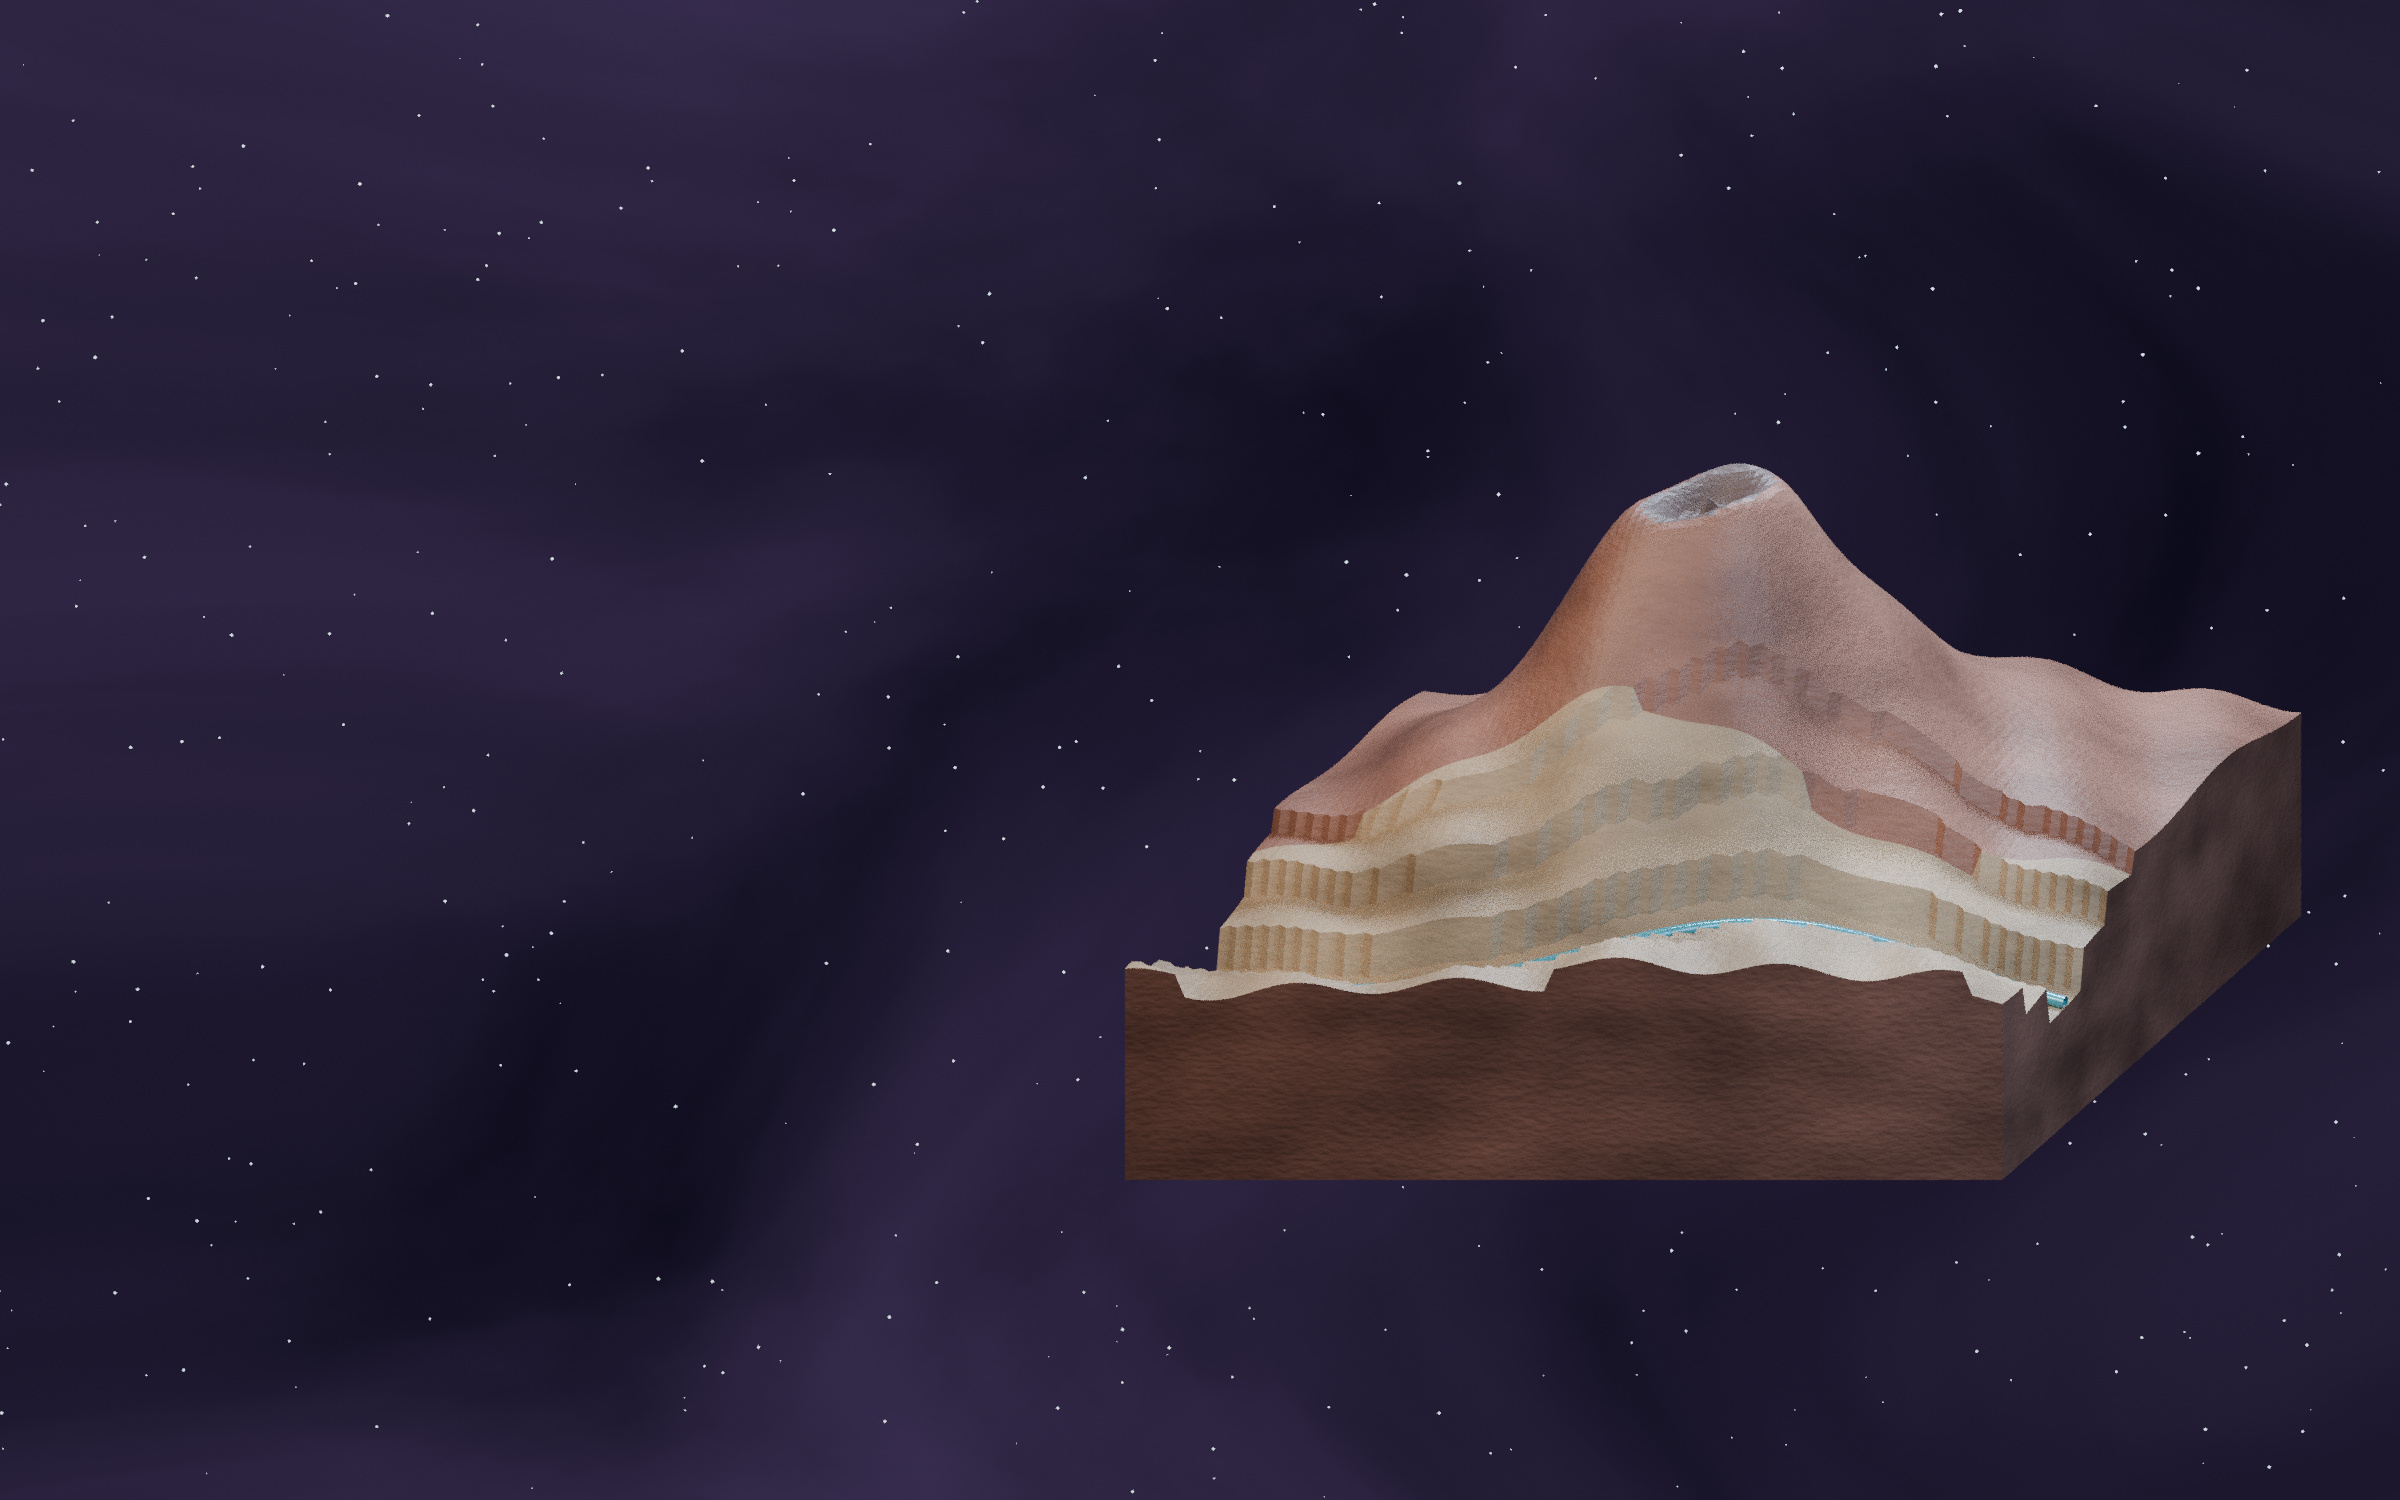
\includegraphics[width=20cm,height=12.5cm]{Scena/copertina.jpg}};}{}
\node[anchor=north west,inner sep=0] at([xshift=1.05cm,yshift=-1.10cm]current page.north west){\color{Mint}\bfseries\fontsize{23}{28}\selectfont IGNIS};
\node[anchor=north west,inner sep=0] at([xshift=1.07cm,yshift=-2.16cm]current page.north west){\color{white}\fontsize{9}{12}\selectfont MODULO M14 · SCIENZE DELLA TERRA};
\draw[Mint,line width=1.5pt]([xshift=1.07cm,yshift=-2.78cm]current page.north west)--([xshift=2.6cm,yshift=-2.78cm]current page.north west);
\node[anchor=north west,inner sep=0] at([xshift=1.05cm,yshift=-3.35cm]current page.north west){\begin{minipage}{9.2cm}\raggedright\color{white}\bfseries\fontsize{28.5}{34.5}\selectfont Estremi, pericolosità\\e rischio\end{minipage}};
\node[anchor=north west,inner sep=0] at([xshift=1.07cm,yshift=-7.88cm]current page.north west){\begin{minipage}{8.9cm}\raggedright\color{Lilac}\fontsize{12.2}{17}\selectfont Il registro delle piene\end{minipage}};
\node[anchor=north west,inner sep=0] at([xshift=1.07cm,yshift=-8.70cm]current page.north west){\begin{minipage}{8.9cm}\raggedright\color{white!75}\fontsize{10.3}{14.5}\selectfont Massimi annuali, livelli rari e conseguenze\end{minipage}};
\node[anchor=north west,inner sep=0] at([xshift=1.07cm,yshift=-10.52cm]current page.north west){\color{white}\fontsize{10.5}{14}\selectfont GeoStat Lab · corso di Marzio De Corato};
\node[anchor=north west,inner sep=0] at([xshift=1.07cm,yshift=-11.17cm]current page.north west){\color{Mint}\fontsize{8.8}{11}\selectfont\href{https://creativecommons.org/licenses/by-nc-sa/4.0/}{Impaginazione da Tessera · CC BY-NC-SA 4.0}};
\end{tikzpicture}\end{frame}
\begin{frame}[plain]\hypertarget{slide2}{}
\bookmark[level=1,page=2]{Indice della presentazione}
\begin{tikzpicture}[remember picture,overlay]
\PilotChrome{Indice della presentazione}{PERCORSO}{2}{I titoli dell’indice aprono i capitoli. Il nome del capitolo in alto riporta a questa pagina.}
\node[anchor=north west,inner sep=0] at([xshift=.96cm,yshift=-2.12cm]current page.north west){\Colonna{9.40cm}{\PLabel{Capitoli}
{\fontsize{10.7}{13.5}\selectfont\hyperlink{slide4}{Massimi annuali e probabilità empiriche\hfill 4}\par}\vspace{.16cm}
{\fontsize{10.7}{13.5}\selectfont\hyperlink{slide14}{Ritorno, attesa e orizzonte temporale\hfill 14}\par}\vspace{.16cm}
{\fontsize{10.7}{13.5}\selectfont\hyperlink{slide24}{Modello Gumbel e verifica dell’adattamento\hfill 24}\par}\vspace{.16cm}
{\fontsize{10.7}{13.5}\selectfont\hyperlink{slide34}{Livelli rari e incertezza della stima\hfill 34}\par}\vspace{.16cm}
{\fontsize{10.7}{13.5}\selectfont\hyperlink{slide45}{Forma della coda e sensibilità GEV\hfill 45}\par}\vspace{.16cm}
{\fontsize{10.7}{13.5}\selectfont\hyperlink{slide51}{Superamenti giornalieri ed episodi\hfill 51}\par}\vspace{.16cm}
{\fontsize{10.7}{13.5}\selectfont\hyperlink{slide58}{Pericolosità, conseguenze e comunicazione\hfill 58}\par}\vspace{.16cm}
}};
\node[anchor=north west,inner sep=0] at([xshift=10.85cm,yshift=-2.12cm]current page.north west){\Colonna{8.16cm}{\PLabel{Percorso di lettura}
\PBody{Il caso principale usa cento massimi annuali sintetici di portata, dal 1920 al 2019. Dal rango degli eventi passiamo al modello di coda e alle sue ipotesi.}
\PInfo{Le pagine Scenario A e Confronto riprendono gli esperimenti nel browser. I valori di partenza del simulatore possono differire dal caso guida.}
\href{https://marzione00.github.io/Lab_Geo/\#modulo-M14}{\color{Classical}\bfseries Apri gli esperimenti di Ignis}}};
\end{tikzpicture}\end{frame}

\begin{frame}[plain]\hypertarget{slide3}{}
\bookmark[level=1,page=3]{Quale portata associamo a un superamento con probabilità annua dell’uno per cento?}
\begin{tikzpicture}[remember picture,overlay]
\PilotChrome{{\fontsize{15.3}{19}\selectfont Quale portata associamo a un superamento con probabilità annua dell’uno per cento?}}{IL CASO GUIDA}{3}{La copertina illustra un bacino. Il record analizzato è una serie sintetica di massimi annuali.}
\node[anchor=north west,inner sep=0] at([xshift=.96cm,yshift=-2.12cm]current page.north west){\Colonna{9.40cm}{{\centering\resizebox{.97\linewidth}{!}{\begin{tikzpicture}[x=1cm,y=1cm]

\draw[pAxis] (.5,.3)--(8,.3) node[below left,pNote]{anno};
\draw[pAxis] (.5,.3)--(.5,4.6) node[above right,pNote]{massimo annuale};
\foreach \x/\h in {1/1.25,2/2.8,3/1.8,4/3.9,5/1.55,6/3.35,7/2.1}{
 \fill[GeoA!52] (\x-.22,.3) rectangle(\x+.22,\h);
 \ifdim\h pt>3pt \fill[GeoB] (\x-.22,3.0) rectangle(\x+.22,\h);\fi}
\draw[GeoB,very thick,dashed] (.5,3)--(7.6,3);
\node[anchor=west,pNote,fill=Paper] at (.8,3.35){soglia $u$};
\node[pNote] at(4.2,-.62){Sette anni illustrativi, due superamenti.};

\end{tikzpicture}
}\par}
}};
\node[anchor=north west,inner sep=0] at([xshift=10.85cm,yshift=-2.12cm]current page.north west){\Colonna{8.16cm}{\PLabel{Il caso}
\PBody{Il caso principale usa cento massimi annuali sintetici di portata, dal 1920 al 2019. Dal rango degli eventi passiamo al modello di coda e alle sue ipotesi.}
\PInfo{Seguiremo la stessa soglia dal singolo anno a un orizzonte di progetto, per distinguere probabilità, frequenza attesa e danno.}
}};
\end{tikzpicture}\end{frame}

\begin{frame}[plain]\hypertarget{slide4}{}
\bookmark[level=0,page=4]{Massimi annuali e probabilità empiriche}
\bookmark[level=1,page=4]{Un anno contribuisce con un solo massimo}
\begin{tikzpicture}[remember picture,overlay]
\PilotChrome{Un anno contribuisce con un solo massimo}{MASSIMI ANNUALI E PROBABILITÀ EMPIRICHE}{4}{Definisci durata e completezza dei blocchi prima di confrontarli.}
\node[anchor=north west,inner sep=0] at([xshift=.96cm,yshift=-2.12cm]current page.north west){\Colonna{9.40cm}{\PLabel{Domanda}
\PBody{Due stagioni sintetiche registrano quattro portate ciascuna. Quali valori entrano nell’analisi dei massimi per blocchi?}
\vspace{.35cm}\PLabel{Interpretazione}
\PBody{Ogni stagione produce un estremo. Periodi di osservazione differenti cambierebbero le opportunità di registrare un picco.}
}};
\node[anchor=north west,inner sep=0] at([xshift=10.85cm,yshift=-2.12cm]current page.north west){\Colonna{8.16cm}{\begin{tcolorbox}[enhanced,arc=1.7mm,boxrule=.6pt,colback=white,colframe=Classical!60!Navy,colbacktitle=Navy,coltitle=white,fonttitle=\bfseries\small,title={R · calcolo riproducibile},left=1.7mm,right=1.3mm,top=1.1mm,bottom=1.1mm,before skip=1mm,after skip=1.0mm]\lstinputlisting[style=GeoR,language=R]{Codice/capitolo-01.R}\end{tcolorbox}
\PLabel{Risultato in R}
\begin{tcolorbox}[colback=GeoTint,colframe=Rule,boxrule=.5pt,arc=1.4mm,left=2mm,right=1mm,top=1mm,bottom=1mm]{\fontsize{9}{12}\selectfont\ttfamily \mbox{1\ \ 2\ }\\\mbox{23\ 28}}\end{tcolorbox}}};
\end{tikzpicture}\end{frame}

\begin{frame}[plain]\hypertarget{slide5}{}
\bookmark[level=1,page=5]{La variabile estrema e l’unità temporale}
\begin{tikzpicture}[remember picture,overlay]
\PilotChrome{La variabile estrema e l’unità temporale}{MASSIMI ANNUALI E PROBABILITÀ EMPIRICHE}{5}{La definizione del blocco temporale determina la variabile alla quale si applica il modello degli estremi.}
\node[anchor=north west,inner sep=0] at([xshift=.96cm,yshift=-2.12cm]current page.north west){\Colonna{9.40cm}{{\centering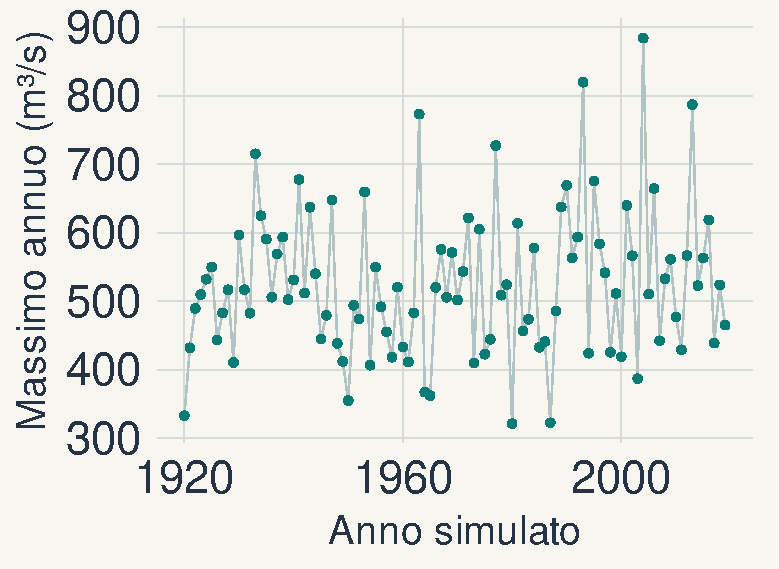
\includegraphics[width=\linewidth,height=6.15cm,keepaspectratio]{Figure/F01.pdf}\par}
\PSmall{Cento massimi annuali simulati, in metri cubi al secondo. Gli anni sono etichette del caso didattico.}
}};
\node[anchor=north west,inner sep=0] at([xshift=10.85cm,yshift=-2.12cm]current page.north west){\Colonna{8.16cm}{\PBody{La serie comprende cento massimi annuali di portata sintetici, associati agli anni dal 1920 al 2019. Ogni riga rappresenta il maggiore valore di un anno e possiede quindi un significato diverso da una portata media annua o da una misura giornaliera. Prima della modellazione si verificano unicità degli anni, continuità del calendario, unità e valori mancanti. La completezza della tabella rende ricostruibile la sequenza, mentre indipendenza e stazionarietà riguardano proprietà del processo che richiedono una valutazione distinta.}
\par\smallskip{\centering\adjustbox{max width=.98\linewidth}{$\displaystyle M_y=\max_{t\in\text{anno }y}Q_t$}\par\smallskip}
}};
\end{tikzpicture}\end{frame}

\begin{frame}[plain]\hypertarget{slide6}{}
\bookmark[level=1,page=6]{Distribuzione del massimo di un blocco}
\begin{tikzpicture}[remember picture,overlay]
\PilotChrome{Distribuzione del massimo di un blocco}{MASSIMI ANNUALI E PROBABILITÀ EMPIRICHE}{6}{La distribuzione di un massimo dipende dalla dimensione e dalla struttura del blocco.}
\node[anchor=north west,inner sep=0] at([xshift=.96cm,yshift=-2.12cm]current page.north west){\Colonna{9.40cm}{{\centering\resizebox{.97\linewidth}{!}{\begin{tikzpicture}[x=1cm,y=-.87cm,every node/.style={font=\fontsize{12.2}{15}\selectfont,text=Ink},arr/.style={-{Stealth[length=2mm]},line width=.8pt,draw=Classical}]\path[use as bounding box] (0,0) rectangle (7.45,6.2);
\draw[draw=Classical,fill=Classical!8,rounded corners=2pt,line width=.7pt] (0.5,1.1) rectangle (1.65,3.2);
\node[anchor=center,text=Ink,font=\fontsize{11}{15}\selectfont,text width=1cm,align=center] at (1.075,2.15) {$Q_1$};
\draw[draw=Classical,fill=Classical!8,rounded corners=2pt,line width=.7pt] (1.85,1.1) rectangle (3.0,3.2);
\node[anchor=center,text=Ink,font=\fontsize{11}{15}\selectfont,text width=1cm,align=center] at (2.425,2.15) {$Q_2$};
\draw[draw=Classical,fill=Classical!8,rounded corners=2pt,line width=.7pt] (3.2,1.1) rectangle (4.35,3.2);
\node[anchor=center,text=Ink,font=\fontsize{11}{15}\selectfont,text width=1cm,align=center] at (3.7750000000000004,2.15) {$\cdots$};
\draw[draw=Classical,fill=Classical!8,rounded corners=2pt,line width=.7pt] (4.550000000000001,1.1) rectangle (5.700000000000001,3.2);
\node[anchor=center,text=Ink,font=\fontsize{11}{15}\selectfont,text width=1cm,align=center] at (5.125000000000001,2.15) {$Q_m$};
\draw[arr,draw=Classical] (3.1,3.5)--(3.1,4.3);
\node[anchor=center,text=Ink,font=\fontsize{12.2}{15}\selectfont,text width=6.8cm,align=center] at (3.7,5.1) {$M_m=\max(Q_1,\ldots,Q_m)$};

\end{tikzpicture}}\par}
}};
\node[anchor=north west,inner sep=0] at([xshift=10.85cm,yshift=-2.12cm]current page.north west){\Colonna{8.16cm}{\PBody{Se un blocco contenesse m osservazioni indipendenti con la medesima distribuzione F, la probabilità che il massimo sia inferiore a una soglia coinciderebbe con la probabilità che tutte le osservazioni lo siano. Il prodotto delle probabilità produce la potenza m della distribuzione originaria. Questa derivazione chiarisce come l’operazione di massimo modifichi la distribuzione; per serie idrologiche reali, dipendenza e stagionalità impediscono spesso di applicare direttamente la formula. La modellazione dei massimi annuali affronta il blocco come unità di analisi.}
\par\smallskip{\centering\adjustbox{max width=.98\linewidth}{$\displaystyle P(M_m\le q)=P(Q_1\le q,\ldots,Q_m\le q)=F(q)^m$}\par\smallskip}
}};
\end{tikzpicture}\end{frame}

\begin{frame}[plain]\hypertarget{slide7}{}
\bookmark[level=1,page=7]{Posizioni empiriche di superamento}
\begin{tikzpicture}[remember picture,overlay]
\PilotChrome{Posizioni empiriche di superamento}{MASSIMI ANNUALI E PROBABILITÀ EMPIRICHE}{7}{Una posizione grafica ordina l’evidenza osservata e conserva l’incertezza dei ranghi estremi.}
\node[anchor=north west,inner sep=0] at([xshift=.96cm,yshift=-2.12cm]current page.north west){\Colonna{9.40cm}{{\centering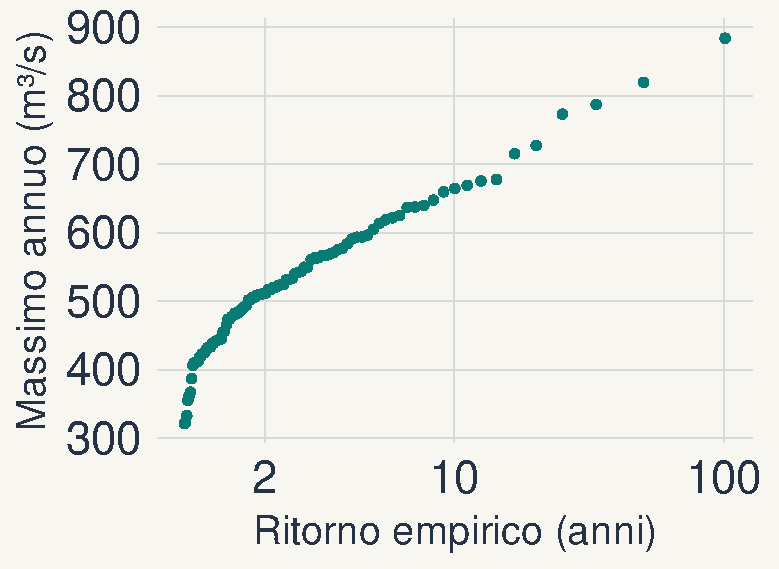
\includegraphics[width=\linewidth,height=6.15cm,keepaspectratio]{Figure/F02.pdf}\par}
\PSmall{n = 100; r = 1 per il massimo, 100 per il minimo. p è la posizione di superamento; T il suo inverso in anni, su scala logaritmica.}
}};
\node[anchor=north west,inner sep=0] at([xshift=10.85cm,yshift=-2.12cm]current page.north west){\Colonna{8.16cm}{\PBody{Ordinando i massimi in senso decrescente, si attribuisce al rango r la posizione grafica r diviso n più uno. L’inverso fornisce una scala convenzionale di ritorno sulla quale rappresentare i dati osservati. Il massimo del record occupa così una posizione prossima a centouno anni, senza diventare una stima certa della probabilità dell’evento. Altre convenzioni di posizione grafica possono modificare leggermente i punti, soprattutto agli estremi; la scelta deve essere dichiarata quando si confrontano grafici o software.}
\par\smallskip{\centering\adjustbox{max width=.98\linewidth}{$\displaystyle \widehat p_r=\frac{r}{n+1},\qquad\widehat T_r=\frac{n+1}{r}$}\par\smallskip}
}};
\end{tikzpicture}\end{frame}

\begin{frame}[plain]\hypertarget{slide8}{}
\bookmark[level=1,page=8]{Distribuzione empirica e soglia di superamento}
\begin{tikzpicture}[remember picture,overlay]
\PilotChrome{Distribuzione empirica e soglia di superamento}{MASSIMI ANNUALI E PROBABILITÀ EMPIRICHE}{8}{La convenzione sulla soglia deve essere identica nel conteggio, nel modello e nella comunicazione del risultato.}
\node[anchor=north west,inner sep=0] at([xshift=.96cm,yshift=-2.12cm]current page.north west){\Colonna{9.40cm}{\begin{tcolorbox}[enhanced,arc=1.7mm,boxrule=.6pt,colback=white,colframe=Classical!60!Navy,colbacktitle=Navy,coltitle=white,fonttitle=\bfseries\small,title={R · procedura},left=1.7mm,right=1.3mm,top=1.1mm,bottom=1.1mm,before skip=1mm,after skip=1.0mm]\lstinputlisting[style=GeoR,language=R]{Codice/lettura-06.R}\end{tcolorbox}
\par\smallskip{\centering\adjustbox{max width=.98\linewidth}{$\displaystyle \widehat F_n(q)=\frac1n\sum_i\mathbf1\{M_i\le q\}\qquad\widehat p(q)=1-\widehat F_n(q)$}\par\smallskip}
}};
\node[anchor=north west,inner sep=0] at([xshift=10.85cm,yshift=-2.12cm]current page.north west){\Colonna{8.16cm}{\PBody{La distribuzione empirica conta la frazione dei massimi minori o uguali alla soglia, mentre il suo complemento conta quelli strettamente maggiori. La distinzione sull’uguaglianza diventa rilevante quando le misure sono arrotondate e compaiono pareggi. Il codice esplicita entrambi gli eventi e verifica che le proporzioni sommino a uno. La frequenza campionaria ottenuta descrive il record disponibile; la sua interpretazione come probabilità del processo richiede che il campione sia pertinente al periodo e al regime di interesse.}
\PInfo{M indica il massimo annuale; n = 100 anni. Nel codice la soglia q è 600 m³/s.}
}};
\end{tikzpicture}\end{frame}

\begin{frame}[plain]\hypertarget{slide9}{}
\bookmark[level=1,page=9]{Quantili campionari e limite del supporto osservato}
\begin{tikzpicture}[remember picture,overlay]
\PilotChrome{Quantili campionari e limite del supporto osservato}{MASSIMI ANNUALI E PROBABILITÀ EMPIRICHE}{9}{L’estrapolazione richiede ipotesi ulteriori e un’analisi della loro influenza.}
\node[anchor=north west,inner sep=0] at([xshift=.96cm,yshift=-2.12cm]current page.north west){\Colonna{9.40cm}{\PLabel{Metodo}
\PBody{Un quantile campionario interpolato, come quello di tipo sette in R, combina valori ordinati del record e rimane entro il loro intervallo. Per probabilità molto elevate, il risultato dipende da pochi massimi e non costruisce automaticamente una coda oltre il valore più grande osservato. Un modello parametrico può produrre quantili esterni al supporto campionario, introducendo ipotesi sulla forma della distribuzione. Il confronto deve quindi distinguere la sintesi dei dati dall’estrapolazione modellistica e riportare la convenzione utilizzata per i quantili empirici.}
}};
\node[anchor=north west,inner sep=0] at([xshift=10.85cm,yshift=-2.12cm]current page.north west){\Colonna{8.16cm}{\PLabel{Formalismo}
\par\smallskip{\centering\adjustbox{max width=.98\linewidth}{$\displaystyle \min_iM_i\le\widehat Q_n(u)\le\max_iM_i\qquad(0\le u\le1)$}\par\smallskip}
\PLabel{Interpretazione}
\PBody{Con cento massimi annuali, una probabilità di superamento dell’ordine di un millesimo riguarda eventi più rari della risoluzione empirica del record. Il numero restituito da una formula deve essere valutato rispetto alla distanza dall’informazione osservata.}
}};
\end{tikzpicture}\end{frame}

\begin{frame}[plain]\hypertarget{slide10}{}
\bookmark[level=1,page=10]{Cento anni definiscono il record osservato}
\begin{tikzpicture}[remember picture,overlay]
\PilotChrome{Cento anni definiscono il record osservato}{MASSIMI ANNUALI E PROBABILITÀ EMPIRICHE}{10}{Il record sintetico comprende un massimo per ciascun anno dal 1920 al 2019.}
\node[anchor=north west,inner sep=0] at([xshift=.96cm,yshift=-2.12cm]current page.north west){\Colonna{9.40cm}{\PLabel{Risultati del calcolo in R}
{\fontsize{10.2}{12.8}\selectfont\begin{tabular}{@{}>{\raggedright\arraybackslash}p{0.52\linewidth}@{\hspace{.13cm}}>{\raggedright\arraybackslash}p{0.39\linewidth}@{}}\toprule Grandezza & Valore\\[2.3pt]
\midrule 
Numero & 100\\[2.3pt]
Dal & 1920\\[2.3pt]
Al & 2019\\[2.3pt]
massimo & 883,69\\[2.3pt]
\bottomrule\end{tabular}\par}
}};
\node[anchor=north west,inner sep=0] at([xshift=10.85cm,yshift=-2.12cm]current page.north west){\Colonna{8.16cm}{\PBody{Qual è la massima portata contenuta nell’intervallo di osservazione?}
\vspace{.4cm}\PInfo{Il record sintetico comprende un massimo per ciascun anno dal 1920 al 2019. La portata massima osservata è il riferimento con cui confrontare i livelli estrapolati.}
}};
\node[anchor=north east,inner sep=0] at([xshift=17.1cm,yshift=-12.04cm]current page.north west){\fontsize{7.7}{9}\selectfont \href{https://github.com/marzione00/Lab_Geo/blob/649f7cc577b96bd1044d81e78a2f530813e4f96b/materiali/laboratori/M14/M14_N01.R}{\color{Classical}\bfseries Script R · M14\_N01}};
\end{tikzpicture}\end{frame}

\begin{frame}[plain]\hypertarget{slide11}{}
\bookmark[level=1,page=11]{Il rango del maggiore dei cento massimi}
\begin{tikzpicture}[remember picture,overlay]
\PilotChrome{Il rango del maggiore dei cento massimi}{MASSIMI ANNUALI E PROBABILITÀ EMPIRICHE}{11}{Con cento anni e rango uno la probabilità di superamento è 1/101.}
\node[anchor=north west,inner sep=0] at([xshift=.96cm,yshift=-2.12cm]current page.north west){\Colonna{9.40cm}{\PLabel{Risultati del calcolo in R}
{\fontsize{10.2}{12.8}\selectfont\begin{tabular}{@{}>{\raggedright\arraybackslash}p{0.22\linewidth}@{\hspace{.13cm}}>{\raggedright\arraybackslash}p{0.22\linewidth}@{\hspace{.13cm}}>{\raggedright\arraybackslash}p{0.22\linewidth}@{\hspace{.13cm}}>{\raggedright\arraybackslash}p{0.23\linewidth}@{}}\toprule rango & portata & Prob. sup. & T\\[2.3pt]
\midrule 
1 & 883,69 & 0,009901 & 101\\[2.3pt]
2 & 819,4 & 0,019802 & 50,5\\[2.3pt]
51 & 511,18 & 0,50495 & 1,9804\\[2.3pt]
99 & 322,54 & 0,9802 & 1,0202\\[2.3pt]
100 & 321,33 & 0,9901 & 1,01\\[2.3pt]
\bottomrule\end{tabular}\par}
\PSmall{Selezione di cinque righe dal file completo.}
}};
\node[anchor=north west,inner sep=0] at([xshift=10.85cm,yshift=-2.12cm]current page.north west){\Colonna{8.16cm}{\PBody{Quale probabilità empirica si associa al primo massimo con la posizione di Weibull?}
\vspace{.4cm}\PInfo{Con cento anni e rango uno la probabilità di superamento è 1/101. Il corrispondente tempo di ritorno dipende dalla convenzione usata per la posizione empirica.}
}};
\node[anchor=north east,inner sep=0] at([xshift=17.1cm,yshift=-12.04cm]current page.north west){\fontsize{7.7}{9}\selectfont \href{https://github.com/marzione00/Lab_Geo/blob/649f7cc577b96bd1044d81e78a2f530813e4f96b/materiali/laboratori/M14/M14_N02.R}{\color{Classical}\bfseries Script R · M14\_N02}};
\end{tikzpicture}\end{frame}

\begin{frame}[plain]\hypertarget{slide12}{}
\bookmark[level=1,page=12]{Dalle osservazioni ai massimi annuali}
\begin{tikzpicture}[remember picture,overlay]
\PilotChrome{Dalle osservazioni ai massimi annuali}{MASSIMI ANNUALI E PROBABILITÀ EMPIRICHE}{12}{Esaminare la distribuzione dei massimi di blocchi indipendenti.}
\node[anchor=north west,inner sep=0] at([xshift=.96cm,yshift=-2.12cm]current page.north west){\Colonna{9.40cm}{{\centering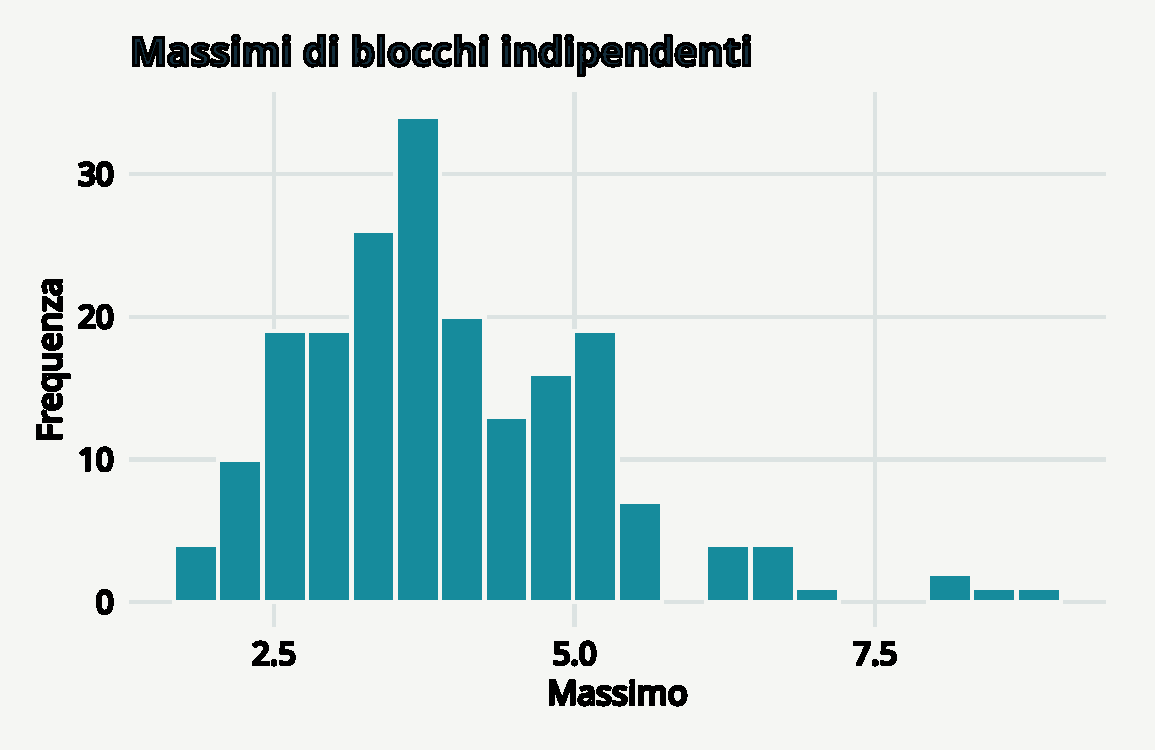
\includegraphics[width=\linewidth,height=6.0cm,keepaspectratio]{Esperimenti/m14-massimi-A.pdf}\par}
\PSmall{Osservazioni per blocco: 30. Seme: 17.}
}};
\node[anchor=north west,inner sep=0] at([xshift=10.85cm,yshift=-2.12cm]current page.north west){\Colonna{8.16cm}{\PLabel{Scenario A · simulazione}
\PBody{Il massimo di un blocco dipende sia dalla distribuzione delle singole osservazioni sia dal numero di occasioni nelle quali possono comparire valori elevati. L’esperimento genera osservazioni esponenziali indipendenti con tasso unitario, raggruppandole in blocchi della dimensione scelta. Per ciascuna replica conserva soltanto il massimo, del quale mostra la distribuzione empirica.}
\par\smallskip{\centering\adjustbox{max width=.98\linewidth}{$\displaystyle P(M_m\le x)=F(x)^m$}\par\smallskip}
\PSmall{$M_m$ è il massimo di m osservazioni indipendenti con la stessa funzione di distribuzione F. La probabilità che il massimo non superi x coincide con la probabilità che tutte le osservazioni non lo superino.}
}};
\node[anchor=north east,inner sep=0] at([xshift=17.1cm,yshift=-12.04cm]current page.north west){\fontsize{7.7}{9}\selectfont \href{https://marzione00.github.io/Lab_Geo/\#laboratorio/m14-massimi}{\color{Classical}\bfseries Apri il laboratorio · m14-massimi}};
\end{tikzpicture}\end{frame}

\begin{frame}[plain]\hypertarget{slide13}{}
\bookmark[level=1,page=13]{Confronto | Dalle osservazioni ai massimi annuali}
\begin{tikzpicture}[remember picture,overlay]
\PilotChrome{Confronto | Dalle osservazioni ai massimi annuali}{MASSIMI ANNUALI E PROBABILITÀ EMPIRICHE}{13}{Il massimo cresce con il numero di opportunità di osservare valori elevati.}
\node[anchor=north west,inner sep=0] at([xshift=.96cm,yshift=-2.12cm]current page.north west){\Colonna{9.40cm}{{\centering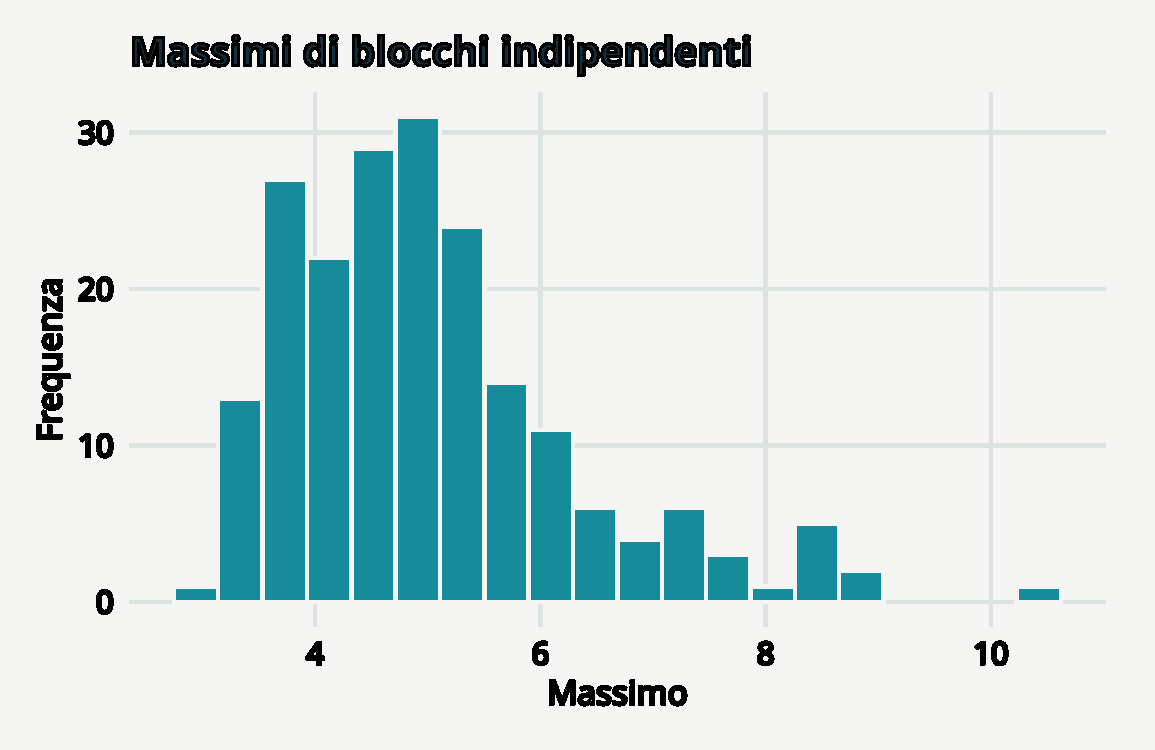
\includegraphics[width=\linewidth,height=5.6cm,keepaspectratio]{Esperimenti/m14-massimi-B.pdf}\par}
\PSmall{Osservazioni per blocco: 30 $\to$ 90. Tutti gli altri parametri e il seme sono fissi.}
}};
\node[anchor=north west,inner sep=0] at([xshift=10.85cm,yshift=-2.12cm]current page.north west){\Colonna{8.16cm}{\PLabel{Confronto fra gli scenari}
{\fontsize{10.2}{12.8}\selectfont\begin{tabular}{@{}>{\raggedright\arraybackslash}p{0.48\linewidth}@{\hspace{.13cm}}>{\raggedright\arraybackslash}p{0.224\linewidth}@{\hspace{.13cm}}>{\raggedright\arraybackslash}p{0.224\linewidth}@{}}\toprule Grandezza & A & B\\[2.3pt]
\midrule 
Media dei massimi & 3,96 & 5,03\\[2.3pt]
Quantile teorico 95\% & 6,37 & 7,47\\[2.3pt]
Quantile empirico 95\% & 6,14 & 7,58\\[2.3pt]
\bottomrule\end{tabular}\par}
\vspace{.25cm}\PBody{Un blocco di 90 osservazioni offre più occasioni per un estremo. La distribuzione di origine è la stessa, mentre la media dei massimi cresce.}
}};
\node[anchor=north east,inner sep=0] at([xshift=17.1cm,yshift=-12.04cm]current page.north west){\fontsize{7.7}{9}\selectfont \href{https://marzione00.github.io/Lab_Geo/\#laboratorio/m14-massimi}{\color{Classical}\bfseries Apri il laboratorio · m14-massimi}};
\end{tikzpicture}\end{frame}

\begin{frame}[plain]\hypertarget{slide14}{}
\bookmark[level=0,page=14]{Ritorno, attesa e orizzonte temporale}
\bookmark[level=1,page=14]{Quanto è probabile almeno una piena in 50 anni?}
\begin{tikzpicture}[remember picture,overlay]
\PilotChrome{Quanto è probabile almeno una piena in 50 anni?}{RITORNO, ATTESA E ORIZZONTE TEMPORALE}{14}{L’orizzonte temporale deve accompagnare la probabilità dichiarata.}
\node[anchor=north west,inner sep=0] at([xshift=.96cm,yshift=-2.12cm]current page.north west){\Colonna{9.40cm}{\PLabel{Domanda}
\PBody{Una soglia ha probabilità annua di superamento pari a 0,01. Consideriamo un orizzonte di 50 anni indipendenti e stazionari.}
\vspace{.35cm}\PLabel{Interpretazione}
\PBody{Il numero atteso è 0,5. La probabilità di almeno un superamento è circa 0,395. Le due quantità rispondono a domande diverse.}
}};
\node[anchor=north west,inner sep=0] at([xshift=10.85cm,yshift=-2.12cm]current page.north west){\Colonna{8.16cm}{\begin{tcolorbox}[enhanced,arc=1.7mm,boxrule=.6pt,colback=white,colframe=Classical!60!Navy,colbacktitle=Navy,coltitle=white,fonttitle=\bfseries\small,title={R · calcolo riproducibile},left=1.7mm,right=1.3mm,top=1.1mm,bottom=1.1mm,before skip=1mm,after skip=1.0mm]\lstinputlisting[style=GeoR,language=R]{Codice/capitolo-02.R}\end{tcolorbox}
\PLabel{Risultato in R}
\begin{tcolorbox}[colback=GeoTint,colframe=Rule,boxrule=.5pt,arc=1.4mm,left=2mm,right=1mm,top=1mm,bottom=1mm]{\fontsize{9}{12}\selectfont\ttfamily \mbox{attesi\ almeno\_uno\ }\\\mbox{\ 0.5000000\ \ 0.3949939}}\end{tcolorbox}}};
\end{tikzpicture}\end{frame}

\begin{frame}[plain]\hypertarget{slide15}{}
\bookmark[level=1,page=15]{Tempo di ritorno e probabilità annua}
\begin{tikzpicture}[remember picture,overlay]
\PilotChrome{Tempo di ritorno e probabilità annua}{RITORNO, ATTESA E ORIZZONTE TEMPORALE}{15}{Il tempo di ritorno è una proprietà probabilistica del modello e della soglia.}
\node[anchor=north west,inner sep=0] at([xshift=.96cm,yshift=-2.12cm]current page.north west){\Colonna{9.40cm}{{\centering\resizebox{.97\linewidth}{!}{\begin{tikzpicture}[x=1cm,y=-.87cm,every node/.style={font=\fontsize{12.2}{15}\selectfont,text=Ink},arr/.style={-{Stealth[length=2mm]},line width=.8pt,draw=Classical}]\path[use as bounding box] (0,0) rectangle (7.45,6.2);
\draw[draw=Classical,fill=Classical!8,rounded corners=2pt,line width=.7pt] (0.5,1.2) rectangle (3.3,3.6);
\node[anchor=center,text=Ink,font=\fontsize{18}{15}\selectfont] at (1.9,2.4) {$p=0,01$};
\draw[arr,draw=Quantum] (3.5,2.4)--(4.1,2.4);
\draw[draw=Quantum,fill=Quantum!8,rounded corners=2pt,line width=.7pt] (4.3,1.2) rectangle (7.1,3.6);
\node[anchor=center,text=Ink,font=\fontsize{18}{15}\selectfont] at (5.7,2.4) {$T=100$};
\node[anchor=center,text=Ink,font=\fontsize{11}{15}\selectfont,text width=6.8cm,align=center] at (3.7,4.6) {Una probabilità annua, espressa in forma inversa.};
\node[anchor=center,text=Ink,font=\fontsize{11}{15}\selectfont,text width=6.8cm,align=center] at (3.7,5.6) {Gli eventi possono essere ravvicinati.};

\end{tikzpicture}}\par}
\PSmall{$F_M(q)=P(M_y\leq q)$: distribuzione del massimo annuale. q: soglia; T: tempo di ritorno in anni. Esempio p = 0,01.}
}};
\node[anchor=north west,inner sep=0] at([xshift=10.85cm,yshift=-2.12cm]current page.north west){\Colonna{8.16cm}{\PBody{Per una soglia fissata e una probabilità annua di superamento costante p, il tempo di ritorno viene definito come il suo inverso. La denominazione centennale corrisponde quindi a p uguale a 0,01 e non impone un intervallo deterministico fra eventi. Due anni consecutivi possono entrambi superare la soglia; nel modello indipendente, l’evento precedente lascia invariata la probabilità del successivo. L’interpretazione richiede di specificare la soglia, il blocco annuale e il regime rispetto al quale la probabilità è considerata stabile.}
\par\smallskip{\centering\adjustbox{max width=.98\linewidth}{$\displaystyle T(q)=\frac1{P(M_y>q)}=\frac1{1-F_M(q)}$}\par\smallskip}
}};
\end{tikzpicture}\end{frame}

\begin{frame}[plain]\hypertarget{slide16}{}
\bookmark[level=1,page=16]{Probabilità di superamento lungo un orizzonte}
\begin{tikzpicture}[remember picture,overlay]
\PilotChrome{Probabilità di superamento lungo un orizzonte}{RITORNO, ATTESA E ORIZZONTE TEMPORALE}{16}{La probabilità sull’intero orizzonte deve essere calcolata sulle condizioni temporali del problema.}
\node[anchor=north west,inner sep=0] at([xshift=.96cm,yshift=-2.12cm]current page.north west){\Colonna{9.40cm}{{\centering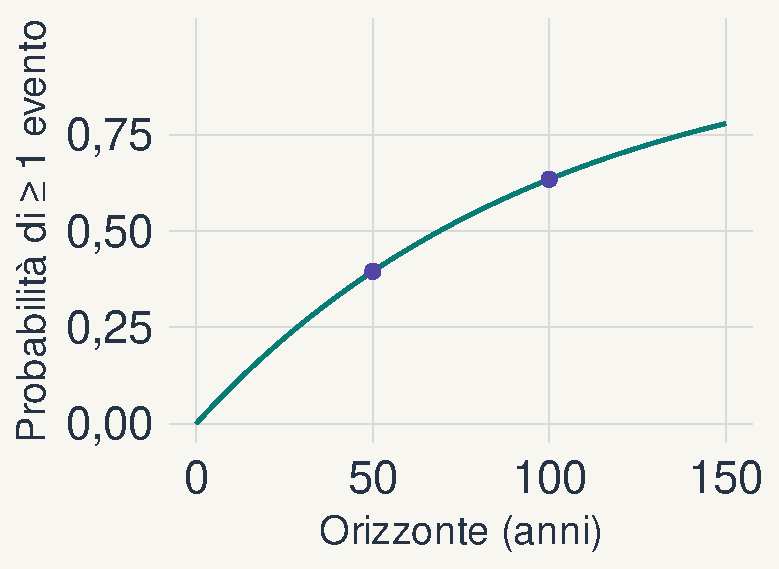
\includegraphics[width=\linewidth,height=6.15cm,keepaspectratio]{Figure/F03.pdf}\par}
\PSmall{$N_H$: numero di anni con superamento entro H anni. Curva per p = 0,01 annuo, con anni indipendenti e probabilità costante.}
}};
\node[anchor=north west,inner sep=0] at([xshift=10.85cm,yshift=-2.12cm]current page.north west){\Colonna{8.16cm}{\PBody{Con anni indipendenti e identica probabilità p, l’assenza di superamenti per H anni ha probabilità pari a uno meno p elevato a H. Il complemento descrive almeno un superamento durante l’intero orizzonte. Per una soglia centennale, la probabilità è circa 39,5\% in cinquant’anni e 63,4\% in cento anni. Il numero atteso di superamenti è invece Hp: le due quantità rispondono a domande differenti e possono assumere valori numericamente molto diversi.}
\par\smallskip{\centering\adjustbox{max width=.98\linewidth}{$\displaystyle P(N_H\ge1)=1-(1-p)^H,\qquad E[N_H]=Hp$}\par\smallskip}
}};
\end{tikzpicture}\end{frame}

\begin{frame}[plain]\hypertarget{slide17}{}
\bookmark[level=1,page=17]{Distribuzione geometrica del tempo di attesa}
\begin{tikzpicture}[remember picture,overlay]
\PilotChrome{Distribuzione geometrica del tempo di attesa}{RITORNO, ATTESA E ORIZZONTE TEMPORALE}{17}{Il valore medio dell’attesa deve essere interpretato insieme alla sua distribuzione.}
\node[anchor=north west,inner sep=0] at([xshift=.96cm,yshift=-2.12cm]current page.north west){\Colonna{9.40cm}{{\centering\resizebox{.97\linewidth}{!}{\begin{tikzpicture}[x=1cm,y=-.87cm,every node/.style={font=\fontsize{12.2}{15}\selectfont,text=Ink},arr/.style={-{Stealth[length=2mm]},line width=.8pt,draw=Classical}]\path[use as bounding box] (0,0) rectangle (7.45,6.2);
\draw[draw=Classical,fill=Classical!8,rounded corners=2pt,line width=.7pt] (0.5,1.3) rectangle (1.55,3.3);
\node[anchor=center,text=Ink,font=\fontsize{16}{15}\selectfont] at (1.025,2.3) {0};
\draw[draw=Classical,fill=Classical!8,rounded corners=2pt,line width=.7pt] (1.8,1.3) rectangle (2.85,3.3);
\node[anchor=center,text=Ink,font=\fontsize{16}{15}\selectfont] at (2.325,2.3) {0};
\draw[draw=Classical,fill=Classical!8,rounded corners=2pt,line width=.7pt] (3.1,1.3) rectangle (4.15,3.3);
\node[anchor=center,text=Ink,font=\fontsize{16}{15}\selectfont] at (3.625,2.3) {0};
\draw[draw=Classical,fill=Classical!8,rounded corners=2pt,line width=.7pt] (4.4,1.3) rectangle (5.45,3.3);
\node[anchor=center,text=Ink,font=\fontsize{16}{15}\selectfont] at (4.925000000000001,2.3) {0};
\draw[draw=Quantum,fill=Quantum!8,rounded corners=2pt,line width=.7pt] (5.7,1.3) rectangle (6.75,3.3);
\node[anchor=center,text=Ink,font=\fontsize{16}{15}\selectfont] at (6.225,2.3) {E};
\node[anchor=center,text=Ink,font=\fontsize{11}{15}\selectfont,text width=6.8cm,align=center] at (3.7,4.4) {Quattro anni senza evento, poi un superamento.};
\node[anchor=center,text=Ink,font=\fontsize{16}{15}\selectfont] at (3.7,5.5) {$P(W=5)=(1-p)^4p$};

\end{tikzpicture}}\par}
}};
\node[anchor=north west,inner sep=0] at([xshift=10.85cm,yshift=-2.12cm]current page.north west){\Colonna{8.16cm}{\PBody{Nel modello di prove annuali indipendenti, l’attesa W fino al primo superamento conta gli anni compreso quello dell’evento. Per attendere esattamente k anni devono verificarsi k meno uno anni senza superamento, seguiti da un anno con superamento. La distribuzione geometrica ha media pari a uno diviso p, mentre la sua asimmetria separa media e mediana. Con p uguale a 0,01 la mediana è sessantanove anni, mentre l’attesa media è cento.}
\par\smallskip{\centering\adjustbox{max width=.98\linewidth}{$\displaystyle P(W=k)=(1-p)^{k-1}p,\quad k=1,2,\ldots$}\par\smallskip}

\par\smallskip{\centering\adjustbox{max width=.98\linewidth}{$\displaystyle E[W]=\frac1p,\qquad\operatorname{Var}(W)=\frac{1-p}{p^2}$}\par\smallskip}
}};
\end{tikzpicture}\end{frame}

\begin{frame}[plain]\hypertarget{slide18}{}
\bookmark[level=1,page=18]{Simulazione delle attese e asimmetria}
\begin{tikzpicture}[remember picture,overlay]
\PilotChrome{Simulazione delle attese e asimmetria}{RITORNO, ATTESA E ORIZZONTE TEMPORALE}{18}{Il conteggio degli insuccessi e quello degli anni fino all’evento differiscono di una unità.}
\node[anchor=north west,inner sep=0] at([xshift=.96cm,yshift=-2.12cm]current page.north west){\Colonna{9.40cm}{{\centering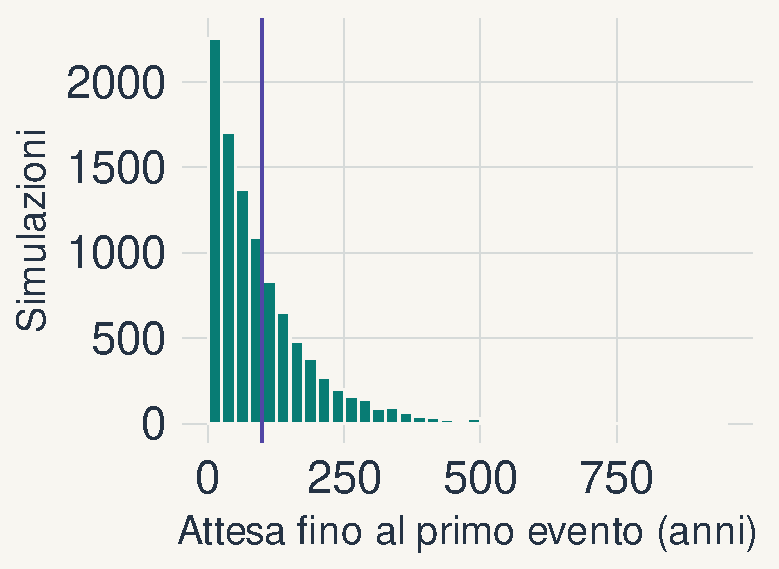
\includegraphics[width=\linewidth,height=6.15cm,keepaspectratio]{Figure/F04.pdf}\par}
\PSmall{Diecimila attese simulate con p = 0,01. La linea viola indica cento anni; il supporto inizia da uno.}
}};
\node[anchor=north west,inner sep=0] at([xshift=10.85cm,yshift=-2.12cm]current page.north west){\Colonna{8.16cm}{\PBody{La simulazione genera diecimila attese indipendenti dal modello geometrico, aggiungendo uno ai valori di rgeom, che conta gli insuccessi prima del primo successo. L’istogramma mostra una concentrazione di attese brevi e una coda di attese lunghe, mentre la linea verticale indica la media teorica di cento anni. La simulazione rende visibile il significato del modello, senza verificare che un processo idrologico reale ne soddisfi le ipotesi. La sequenza casuale e la convenzione di conteggio sono incluse nel codice riproducibile.}
}};
\end{tikzpicture}\end{frame}

\begin{frame}[plain]\hypertarget{slide19}{}
\bookmark[level=1,page=19]{Probabilità variabile e dipendenza fra anni}
\begin{tikzpicture}[remember picture,overlay]
\PilotChrome{Probabilità variabile e dipendenza fra anni}{RITORNO, ATTESA E ORIZZONTE TEMPORALE}{19}{La stazionarietà e l’indipendenza svolgono ruoli distinti nelle formule di probabilità temporale.}
\node[anchor=north west,inner sep=0] at([xshift=.96cm,yshift=-2.12cm]current page.north west){\Colonna{9.40cm}{{\centering\resizebox{.97\linewidth}{!}{\begin{tikzpicture}[x=1cm,y=-.87cm,every node/.style={font=\fontsize{12.2}{15}\selectfont,text=Ink},arr/.style={-{Stealth[length=2mm]},line width=.8pt,draw=Classical}]\path[use as bounding box] (0,0) rectangle (7.45,6.2);
\draw[arr,draw=Classical] (0.6,4.5)--(6.8,4.5);
\draw[draw=Classical,fill=Classical!8,rounded corners=2pt,line width=.7pt] (1.0,3.5) rectangle (1.9,4.5);
\node[anchor=center,text=Ink,font=\fontsize{11}{15}\selectfont] at (1.45,5.1) {$p_1$};
\draw[draw=Classical,fill=Classical!8,rounded corners=2pt,line width=.7pt] (2.5,3.0) rectangle (3.4,4.5);
\node[anchor=center,text=Ink,font=\fontsize{11}{15}\selectfont] at (2.95,5.1) {$p_2$};
\draw[draw=Quantum,fill=Quantum!8,rounded corners=2pt,line width=.7pt] (4.0,2.2) rectangle (4.9,4.5);
\node[anchor=center,text=Ink,font=\fontsize{11}{15}\selectfont] at (4.45,5.1) {$p_3$};
\draw[draw=Quantum,fill=Quantum!8,rounded corners=2pt,line width=.7pt] (5.5,1.5) rectangle (6.4,4.5);
\node[anchor=center,text=Ink,font=\fontsize{11}{15}\selectfont] at (5.95,5.1) {$p_4$};
\node[anchor=center,text=Ink,font=\fontsize{12.2}{15}\selectfont,text width=6.8cm,align=center] at (3.7,0.6) {Probabilità annuali di scenario};

\end{tikzpicture}}\par}
\PSmall{$p_t$: probabilità di superamento nell’anno t; H: durata; $N_H$: conteggio. Il prodotto vale sotto indipendenza, anche con probabilità diverse.}
}};
\node[anchor=north west,inner sep=0] at([xshift=10.85cm,yshift=-2.12cm]current page.north west){\Colonna{8.16cm}{\PBody{Se la probabilità cambia nel tempo ma gli anni restano indipendenti, la probabilità di nessun superamento è il prodotto dei complementi delle probabilità annuali. Un unico tempo di ritorno costante non riassume più l’intero periodo. Quando vi è dipendenza, anche tale prodotto richiede una sostituzione con probabilità condizionate o con un modello congiunto. La valutazione di lungo periodo deve quindi considerare cambiamenti del processo, modifiche del bacino e persistenza, oltre all’incertezza nella stima dei parametri.}
\par\smallskip{\centering\adjustbox{max width=.98\linewidth}{$\displaystyle P(N_H\ge1)=1-\prod_{t=1}^{H}(1-p_t)$}\par\smallskip}
}};
\end{tikzpicture}\end{frame}

\begin{frame}[plain]\hypertarget{slide20}{}
\bookmark[level=1,page=20]{Probabilità ed eventi attesi crescono in modo diverso}
\begin{tikzpicture}[remember picture,overlay]
\PilotChrome{Probabilità ed eventi attesi crescono in modo diverso}{RITORNO, ATTESA E ORIZZONTE TEMPORALE}{20}{Il numero atteso cresce linearmente con gli anni.}
\node[anchor=north west,inner sep=0] at([xshift=.96cm,yshift=-2.12cm]current page.north west){\Colonna{9.40cm}{\PLabel{Risultati del calcolo in R}
{\fontsize{10.2}{12.8}\selectfont\begin{tabular}{@{}>{\raggedright\arraybackslash}p{0.31\linewidth}@{\hspace{.13cm}}>{\raggedright\arraybackslash}p{0.29\linewidth}@{\hspace{.13cm}}>{\raggedright\arraybackslash}p{0.32\linewidth}@{}}\toprule anni & almeno uno & eventi attesi\\[2.3pt]
\midrule 
1 & 0,01 & 0,01\\[2.3pt]
10 & 0,095618 & 0,1\\[2.3pt]
30 & 0,2603 & 0,3\\[2.3pt]
50 & 0,39499 & 0,5\\[2.3pt]
100 & 0,63397 & 1\\[2.3pt]
\bottomrule\end{tabular}\par}
}};
\node[anchor=north west,inner sep=0] at([xshift=10.85cm,yshift=-2.12cm]current page.north west){\Colonna{8.16cm}{\PBody{Come evolve il rischio di almeno un superamento quando si allunga la vita utile?}
\vspace{.4cm}\PInfo{Il numero atteso cresce linearmente con gli anni. La probabilità di almeno un superamento resta compresa fra zero e uno.}
}};
\node[anchor=north east,inner sep=0] at([xshift=17.1cm,yshift=-12.04cm]current page.north west){\fontsize{7.7}{9}\selectfont \href{https://github.com/marzione00/Lab_Geo/blob/649f7cc577b96bd1044d81e78a2f530813e4f96b/materiali/laboratori/M14/M14_N05.R}{\color{Classical}\bfseries Script R · M14\_N05}};
\end{tikzpicture}\end{frame}

\begin{frame}[plain]\hypertarget{slide21}{}
\bookmark[level=1,page=21]{La media dell’attesa è maggiore della mediana}
\begin{tikzpicture}[remember picture,overlay]
\PilotChrome{La media dell’attesa è maggiore della mediana}{RITORNO, ATTESA E ORIZZONTE TEMPORALE}{21}{Una piccola quota di attese molto lunghe sposta la media.}
\node[anchor=north west,inner sep=0] at([xshift=.96cm,yshift=-2.12cm]current page.north west){\Colonna{9.40cm}{\PLabel{Risultati del calcolo in R}
{\fontsize{10.2}{12.8}\selectfont\begin{tabular}{@{}>{\raggedright\arraybackslash}p{0.52\linewidth}@{\hspace{.13cm}}>{\raggedright\arraybackslash}p{0.39\linewidth}@{}}\toprule Grandezza & Valore\\[2.3pt]
\midrule 
media & 100,88\\[2.3pt]
mediana & 71\\[2.3pt]
teorica & 100\\[2.3pt]
quota entro10 & 0,093\\[2.3pt]
\bottomrule\end{tabular}\par}
}};
\node[anchor=north west,inner sep=0] at([xshift=10.85cm,yshift=-2.12cm]current page.north west){\Colonna{8.16cm}{\PBody{In una sequenza di anni indipendenti, quanto si deve aspettare il primo superamento?}
\vspace{.4cm}\PInfo{Una piccola quota di attese molto lunghe sposta la media. La mediana della simulazione e la probabilità entro dieci anni raccontano aspetti diversi della distribuzione.}
}};
\node[anchor=north east,inner sep=0] at([xshift=17.1cm,yshift=-12.04cm]current page.north west){\fontsize{7.7}{9}\selectfont \href{https://github.com/marzione00/Lab_Geo/blob/649f7cc577b96bd1044d81e78a2f530813e4f96b/materiali/laboratori/M14/M14_N06.R}{\color{Classical}\bfseries Script R · M14\_N06}};
\end{tikzpicture}\end{frame}

\begin{frame}[plain]\hypertarget{slide22}{}
\bookmark[level=1,page=22]{Tempo di ritorno e orizzonte temporale}
\begin{tikzpicture}[remember picture,overlay]
\PilotChrome{Tempo di ritorno e orizzonte temporale}{RITORNO, ATTESA E ORIZZONTE TEMPORALE}{22}{Distinguere probabilità annuale, attesa e rischio cumulato.}
\node[anchor=north west,inner sep=0] at([xshift=.96cm,yshift=-2.12cm]current page.north west){\Colonna{9.40cm}{{\centering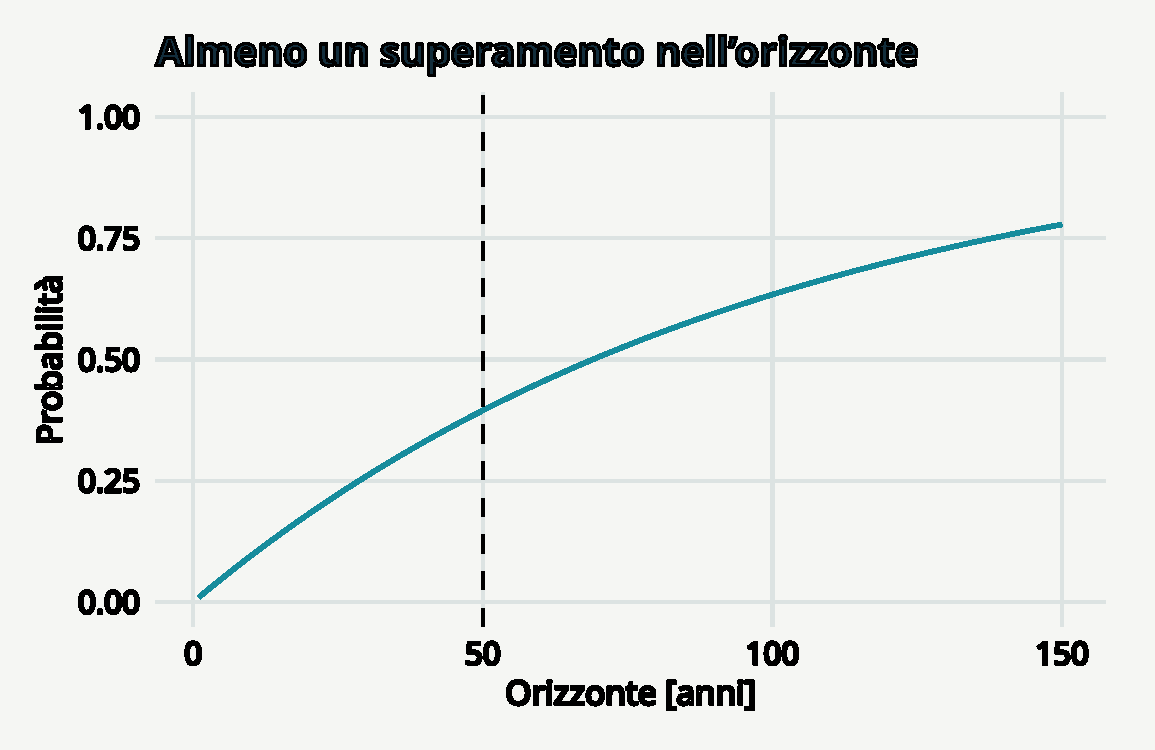
\includegraphics[width=\linewidth,height=6.0cm,keepaspectratio]{Esperimenti/m14-ritorno-A.pdf}\par}
\PSmall{Orizzonte [anni]: 50. Seme: 17.}
}};
\node[anchor=north west,inner sep=0] at([xshift=10.85cm,yshift=-2.12cm]current page.north west){\Colonna{8.16cm}{\PLabel{Scenario A · simulazione}
\PBody{Il tempo di ritorno associa una soglia alla probabilità annuale di superamento, assumendo un regime nel quale tale probabilità rimanga costante. Il controllo imposta questa attesa teorica, mentre l’orizzonte determina per quanti anni viene considerata l’esposizione. La curva mostra la probabilità di osservare almeno un superamento durante ciascun intervallo temporale.}
\par\smallskip{\centering\adjustbox{max width=.98\linewidth}{$\displaystyle P(N_H\ge1)=1-(1-1/T)^H$}\par\smallskip}
\PSmall{T è il tempo di ritorno in anni, p=1/T la probabilità annuale, H la durata dell’orizzonte e $N_H$ il numero di superamenti nel periodo. Il numero atteso è H/T.}
}};
\node[anchor=north east,inner sep=0] at([xshift=17.1cm,yshift=-12.04cm]current page.north west){\fontsize{7.7}{9}\selectfont \href{https://marzione00.github.io/Lab_Geo/\#laboratorio/m14-ritorno}{\color{Classical}\bfseries Apri il laboratorio · m14-ritorno}};
\end{tikzpicture}\end{frame}

\begin{frame}[plain]\hypertarget{slide23}{}
\bookmark[level=1,page=23]{Confronto | Tempo di ritorno e orizzonte temporale}
\begin{tikzpicture}[remember picture,overlay]
\PilotChrome{Confronto | Tempo di ritorno e orizzonte temporale}{RITORNO, ATTESA E ORIZZONTE TEMPORALE}{23}{Il tempo di ritorno è un’attesa del modello e non impone intervalli regolari fra eventi.}
\node[anchor=north west,inner sep=0] at([xshift=.96cm,yshift=-2.12cm]current page.north west){\Colonna{9.40cm}{{\centering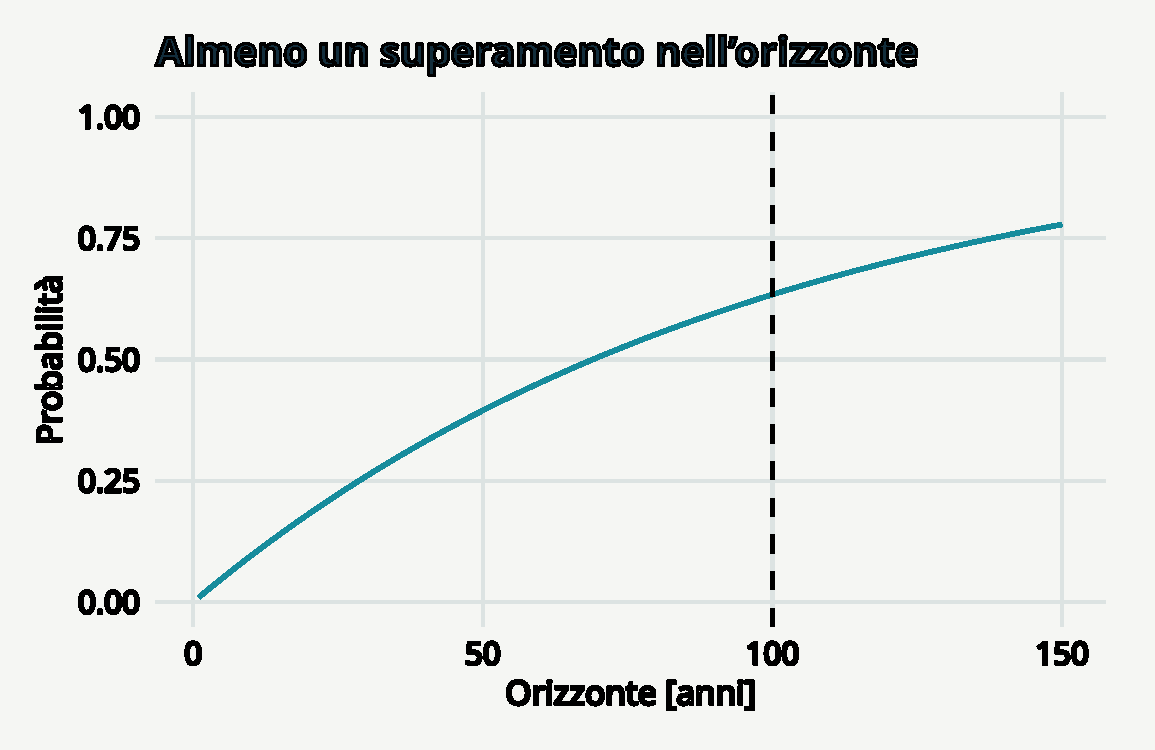
\includegraphics[width=\linewidth,height=5.6cm,keepaspectratio]{Esperimenti/m14-ritorno-B.pdf}\par}
\PSmall{Orizzonte [anni]: 50 $\to$ 100. Tutti gli altri parametri e il seme sono fissi.}
}};
\node[anchor=north west,inner sep=0] at([xshift=10.85cm,yshift=-2.12cm]current page.north west){\Colonna{8.16cm}{\PLabel{Confronto fra gli scenari}
{\fontsize{10.2}{12.8}\selectfont\begin{tabular}{@{}>{\raggedright\arraybackslash}p{0.48\linewidth}@{\hspace{.13cm}}>{\raggedright\arraybackslash}p{0.224\linewidth}@{\hspace{.13cm}}>{\raggedright\arraybackslash}p{0.224\linewidth}@{}}\toprule Grandezza & A & B\\[2.3pt]
\midrule 
Probabilità annuale & 0,01 & 0,01\\[2.3pt]
Probabilità cumulata & 0,395 & 0,634\\[2.3pt]
Numero atteso di superamenti & 0,5 & 1\\[2.3pt]
\bottomrule\end{tabular}\par}
\vspace{.25cm}\PBody{Raddoppiando l’orizzonte da 50 a 100 anni la probabilità cumulata passa da circa 0,395 a 0,634. La probabilità di ciascun anno resta 0,01.}
}};
\node[anchor=north east,inner sep=0] at([xshift=17.1cm,yshift=-12.04cm]current page.north west){\fontsize{7.7}{9}\selectfont \href{https://marzione00.github.io/Lab_Geo/\#laboratorio/m14-ritorno}{\color{Classical}\bfseries Apri il laboratorio · m14-ritorno}};
\end{tikzpicture}\end{frame}

\begin{frame}[plain]\hypertarget{slide24}{}
\bookmark[level=0,page=24]{Modello Gumbel e verifica dell’adattamento}
\bookmark[level=1,page=24]{Ricostruire il quantile attraverso la cumulata}
\begin{tikzpicture}[remember picture,overlay]
\PilotChrome{Ricostruire il quantile attraverso la cumulata}{MODELLO GUMBEL E VERIFICA DELL’ADATTAMENTO}{24}{Un’inversione numerica riuscita verifica il calcolo; l’adattamento ai dati richiede una diagnostica separata.}
\node[anchor=north west,inner sep=0] at([xshift=.96cm,yshift=-2.12cm]current page.north west){\Colonna{9.40cm}{\PLabel{Domanda}
\PBody{In un esempio Gumbel usiamo posizione 476,26 e scala 82,96 m³/s, arrotondate dai massimi annuali del corso. Quale livello lascia il 99\% della distribuzione al di sotto?}
\vspace{.35cm}\PLabel{Interpretazione}
\PBody{Sostituiamo il quantile nella cumulata. Recuperare 0,99 controlla segno e trasformazioni logaritmiche.}
}};
\node[anchor=north west,inner sep=0] at([xshift=10.85cm,yshift=-2.12cm]current page.north west){\Colonna{8.16cm}{\begin{tcolorbox}[enhanced,arc=1.7mm,boxrule=.6pt,colback=white,colframe=Classical!60!Navy,colbacktitle=Navy,coltitle=white,fonttitle=\bfseries\small,title={R · calcolo riproducibile},left=1.7mm,right=1.3mm,top=1.1mm,bottom=1.1mm,before skip=1mm,after skip=1.0mm]\lstinputlisting[style=GeoR,language=R]{Codice/capitolo-03.R}\end{tcolorbox}
\PLabel{Risultato in R}
\begin{tcolorbox}[colback=GeoTint,colframe=Rule,boxrule=.5pt,arc=1.4mm,left=2mm,right=1mm,top=1mm,bottom=1mm]{\fontsize{9}{12}\selectfont\ttfamily \mbox{livello\ \ \ \ \ \ \ \ F\ }\\\mbox{857.8884\ \ \ 0.9900}}\end{tcolorbox}}};
\end{tikzpicture}\end{frame}

\begin{frame}[plain]\hypertarget{slide25}{}
\bookmark[level=1,page=25]{Gumbel per massimi: posizione e scala}
\begin{tikzpicture}[remember picture,overlay]
\PilotChrome{Gumbel per massimi: posizione e scala}{MODELLO GUMBEL E VERIFICA DELL’ADATTAMENTO}{25}{Parametrizzazione, unità e direzione dell’estremo devono essere coerenti in tutte le formule.}
\node[anchor=north west,inner sep=0] at([xshift=.96cm,yshift=-2.12cm]current page.north west){\Colonna{9.40cm}{\PLabel{Metodo}
\PBody{La distribuzione Gumbel per massimi descrive una famiglia con parametro di posizione a e parametro di scala b positivo. La funzione cumulativa aumenta da zero a uno, mentre la trasformazione interna determina una coda destra asimmetrica. Il modello è una possibile approssimazione dei massimi di blocco, la cui pertinenza deve essere valutata rispetto al processo e ai dati. La parametrizzazione per massimi deve essere distinta da quella per minimi, poiché un’inversione dei segni modifica la direzione della coda.}
}};
\node[anchor=north west,inner sep=0] at([xshift=10.85cm,yshift=-2.12cm]current page.north west){\Colonna{8.16cm}{\PLabel{Formalismo}
\par\smallskip{\centering\adjustbox{max width=.98\linewidth}{$\displaystyle F(q)=\exp\!\left[-\exp\!\left(-\frac{q-a}{b}\right)\right],\qquad b>0$}\par\smallskip}
\PLabel{Interpretazione}
\PBody{La media è a + γb e la deviazione standard è bπ/√6, dove γ $\simeq$ 0,577216 è la costante di Eulero–Mascheroni. Nella Gumbel il parametro di posizione e la media hanno valori differenti.}
}};
\end{tikzpicture}\end{frame}

\begin{frame}[plain]\hypertarget{slide26}{}
\bookmark[level=1,page=26]{Stima basata sui momenti campionari}
\begin{tikzpicture}[remember picture,overlay]
\PilotChrome{Stima basata sui momenti campionari}{MODELLO GUMBEL E VERIFICA DELL’ADATTAMENTO}{26}{La procedura di stima e le convenzioni campionarie devono accompagnare i parametri.}
\node[anchor=north west,inner sep=0] at([xshift=.96cm,yshift=-2.12cm]current page.north west){\Colonna{9.40cm}{\begin{tcolorbox}[enhanced,arc=1.7mm,boxrule=.6pt,colback=white,colframe=Classical!60!Navy,colbacktitle=Navy,coltitle=white,fonttitle=\bfseries\small,title={R · procedura},left=1.7mm,right=1.3mm,top=1.1mm,bottom=1.1mm,before skip=1mm,after skip=1.0mm]\lstinputlisting[style=GeoR,language=R]{Codice/lettura-14.R}\end{tcolorbox}
\par\smallskip{\centering\adjustbox{max width=.98\linewidth}{$\displaystyle \widehat b=s\frac{\sqrt6}{\pi},\qquad\widehat a=\overline M-\gamma\widehat b$}\par\smallskip}
}};
\node[anchor=north west,inner sep=0] at([xshift=10.85cm,yshift=-2.12cm]current page.north west){\Colonna{8.16cm}{\PBody{La stima utilizzata nel laboratorio ricava la scala dalla deviazione standard campionaria e la posizione dalla media, sfruttando le relazioni teoriche della Gumbel. La deviazione standard di R impiega il denominatore n meno uno, convenzione che viene mantenuta nel codice. Per il record sintetico si ottengono a circa 476,26 e b circa 82,96 metri cubi al secondo. Questa procedura basata sui momenti è semplice da verificare manualmente e rimane distinta dalla massima verosimiglianza, che richiede un’ottimizzazione della funzione di verosimiglianza.}
\PInfo{$\bar M$: media; s: deviazione campionaria; $\gamma\simeq0{,}577216$: costante di Eulero–Mascheroni. a e b sono posizione e scala.}
}};
\end{tikzpicture}\end{frame}

\begin{frame}[plain]\hypertarget{slide27}{}
\bookmark[level=1,page=27]{Quantile Gumbel e controllo dell’inversione}
\begin{tikzpicture}[remember picture,overlay]
\PilotChrome{Quantile Gumbel e controllo dell’inversione}{MODELLO GUMBEL E VERIFICA DELL’ADATTAMENTO}{27}{Una formula correttamente implementata può restare statisticamente inadeguata al processo studiato.}
\node[anchor=north west,inner sep=0] at([xshift=.96cm,yshift=-2.12cm]current page.north west){\Colonna{9.40cm}{\begin{tcolorbox}[enhanced,arc=1.7mm,boxrule=.6pt,colback=white,colframe=Classical!60!Navy,colbacktitle=Navy,coltitle=white,fonttitle=\bfseries\small,title={R · procedura},left=1.7mm,right=1.3mm,top=1.1mm,bottom=1.1mm,before skip=1mm,after skip=1.0mm]\lstinputlisting[style=GeoR,language=R]{Codice/lettura-15.R}\end{tcolorbox}
\par\smallskip{\centering\adjustbox{max width=.98\linewidth}{$\displaystyle Q(u)=a-b\log[-\log(u)],\qquad F[Q(u)]=u$}\par\smallskip}
}};
\node[anchor=north west,inner sep=0] at([xshift=10.85cm,yshift=-2.12cm]current page.north west){\Colonna{8.16cm}{\PBody{Invertendo la funzione cumulativa si ottiene il quantile per probabilità comprese strettamente fra zero e uno. Il doppio logaritmo rende essenziale il controllo dei segni e del dominio: una probabilità esterna all’intervallo produrrebbe valori indefiniti. Il codice verifica che la composizione della distribuzione con il quantile restituisca le probabilità iniziali entro la tolleranza numerica. Tale identità controlla l’implementazione algebrica e deve essere distinta dall’adeguatezza del modello ai massimi osservati.}
\PInfo{a: posizione; b > 0: scala; u: probabilità cumulativa, con 0 < u < 1. log indica il logaritmo naturale.}
}};
\end{tikzpicture}\end{frame}

\begin{frame}[plain]\hypertarget{slide28}{}
\bookmark[level=1,page=28]{Distribuzione cumulativa empirica e adattata}
\begin{tikzpicture}[remember picture,overlay]
\PilotChrome{Distribuzione cumulativa empirica e adattata}{MODELLO GUMBEL E VERIFICA DELL’ADATTAMENTO}{28}{La concordanza centrale deve essere accompagnata da una verifica della coda pertinente al problema.}
\node[anchor=north west,inner sep=0] at([xshift=.96cm,yshift=-2.12cm]current page.north west){\Colonna{9.40cm}{{\centering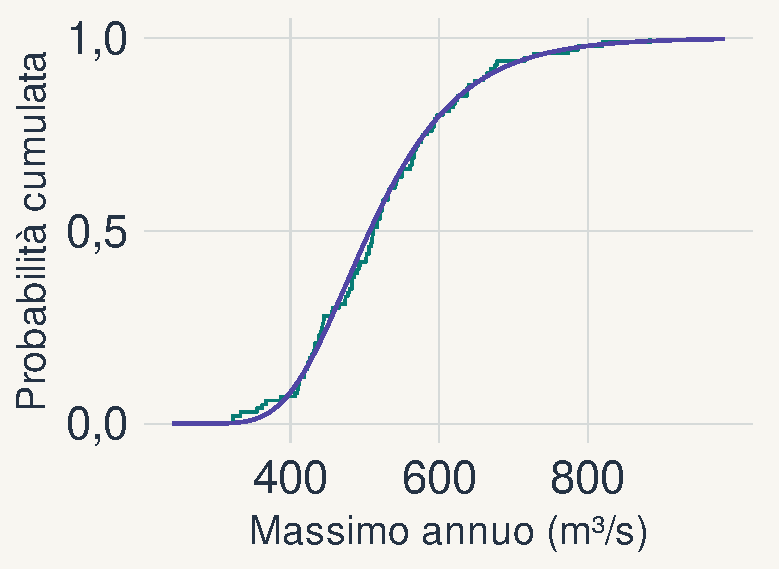
\includegraphics[width=\linewidth,height=6.15cm,keepaspectratio]{Figure/F06.pdf}\par}
\PSmall{Verde: distribuzione empirica dei cento massimi. Viola: Gumbel stimata mediante i momenti campionari.}
}};
\node[anchor=north west,inner sep=0] at([xshift=10.85cm,yshift=-2.12cm]current page.north west){\Colonna{8.16cm}{\PBody{Il confronto sovrappone la funzione empirica, che procede per salti di ampiezza uno su cento, alla distribuzione Gumbel stimata. La corrispondenza complessiva aiuta a riconoscere scostamenti di posizione e dispersione, ma la scala cumulativa può rendere poco evidenti divergenze nella coda estrema. La valutazione deve perciò integrare rappresentazioni mirate ai quantili alti e analisi di sensibilità. La distribuzione empirica e quella adattata utilizzano lo stesso record, circostanza da ricordare nell’interpretazione della concordanza.}
}};
\end{tikzpicture}\end{frame}

\begin{frame}[plain]\hypertarget{slide29}{}
\bookmark[level=1,page=29]{Diagramma quantile–quantile e coda}
\begin{tikzpicture}[remember picture,overlay]
\PilotChrome{Diagramma quantile–quantile e coda}{MODELLO GUMBEL E VERIFICA DELL’ADATTAMENTO}{29}{La coda della distribuzione richiede un esame specifico, proporzionato alla scarsità dell’informazione.}
\node[anchor=north west,inner sep=0] at([xshift=.96cm,yshift=-2.12cm]current page.north west){\Colonna{9.40cm}{{\centering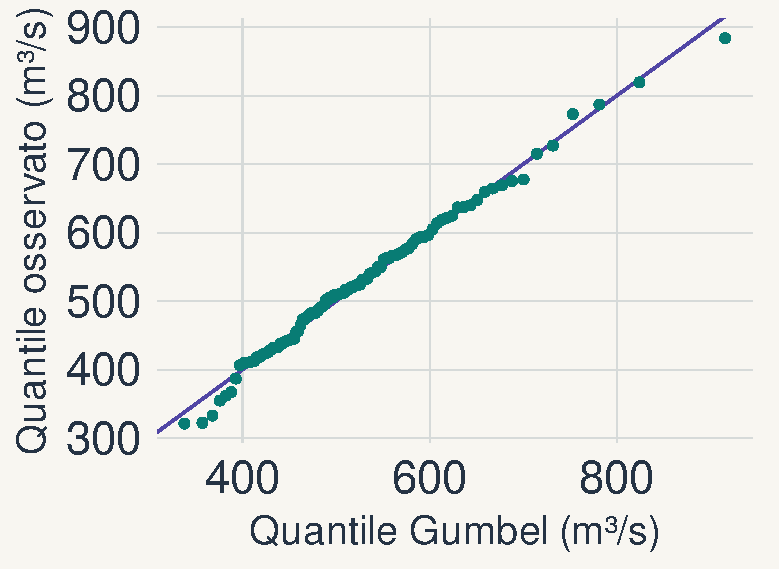
\includegraphics[width=\linewidth,height=6.15cm,keepaspectratio]{Figure/F05.pdf}\par}
\PSmall{Quantili teorici alle posizioni (i – 0,5)/n; la diagonale rappresenta l’uguaglianza fra quantile teorico e osservato.}
}};
\node[anchor=north west,inner sep=0] at([xshift=10.85cm,yshift=-2.12cm]current page.north west){\Colonna{8.16cm}{\PBody{Il diagramma confronta massimi ordinati e quantili Gumbel calcolati alle stesse posizioni di probabilità. Una corrispondenza sulla diagonale indica accordo locale fra le due scale, mentre curvature o scostamenti agli estremi suggeriscono differenze nella forma della distribuzione. I punti di coda sono pochi e variabili, per cui una deviazione isolata richiede un esame dell’evento e della qualità della misura. La diagnostica deve essere collegata ai livelli che si vogliono stimare, poiché un buon adattamento centrale può coesistere con incertezza elevata sui valori rari.}
}};
\end{tikzpicture}\end{frame}

\begin{frame}[plain]\hypertarget{slide30}{}
\bookmark[level=1,page=30]{Due parametri riassumono l’adattamento Gumbel}
\begin{tikzpicture}[remember picture,overlay]
\PilotChrome{Due parametri riassumono l’adattamento Gumbel}{MODELLO GUMBEL E VERIFICA DELL’ADATTAMENTO}{30}{Il metodo dei momenti ricava la scala dalla deviazione standard e corregge la media per stimare la posizione.}
\node[anchor=north west,inner sep=0] at([xshift=.96cm,yshift=-2.12cm]current page.north west){\Colonna{9.40cm}{\PLabel{Risultati del calcolo in R}
{\fontsize{10.2}{12.8}\selectfont\begin{tabular}{@{}>{\raggedright\arraybackslash}p{0.52\linewidth}@{\hspace{.13cm}}>{\raggedright\arraybackslash}p{0.39\linewidth}@{}}\toprule Grandezza & Valore\\[2.3pt]
\midrule 
posizione & 476,26\\[2.3pt]
scala & 82,961\\[2.3pt]
media & 524,15\\[2.3pt]
sd & 106,4\\[2.3pt]
\bottomrule\end{tabular}\par}
}};
\node[anchor=north west,inner sep=0] at([xshift=10.85cm,yshift=-2.12cm]current page.north west){\Colonna{8.16cm}{\PBody{Quale relazione lega media e dispersione dei massimi ai parametri stimati?}
\vspace{.4cm}\PInfo{Il metodo dei momenti ricava la scala dalla deviazione standard e corregge la media per stimare la posizione. Le unità dei parametri sono quelle della portata.}
}};
\node[anchor=north east,inner sep=0] at([xshift=17.1cm,yshift=-12.04cm]current page.north west){\fontsize{7.7}{9}\selectfont \href{https://github.com/marzione00/Lab_Geo/blob/649f7cc577b96bd1044d81e78a2f530813e4f96b/materiali/laboratori/M14/M14_N08.R}{\color{Classical}\bfseries Script R · M14\_N08}};
\end{tikzpicture}\end{frame}

\begin{frame}[plain]\hypertarget{slide31}{}
\bookmark[level=1,page=31]{Una prova numerica dell’inversa Gumbel}
\begin{tikzpicture}[remember picture,overlay]
\PilotChrome{Una prova numerica dell’inversa Gumbel}{MODELLO GUMBEL E VERIFICA DELL’ADATTAMENTO}{31}{Il confronto fra la prima e l’ultima colonna verifica l’implementazione dell’inversa.}
\node[anchor=north west,inner sep=0] at([xshift=.96cm,yshift=-2.12cm]current page.north west){\Colonna{9.40cm}{\PLabel{Risultati del calcolo in R}
{\fontsize{10.2}{12.8}\selectfont\begin{tabular}{@{}>{\raggedright\arraybackslash}p{0.31\linewidth}@{\hspace{.13cm}}>{\raggedright\arraybackslash}p{0.29\linewidth}@{\hspace{.13cm}}>{\raggedright\arraybackslash}p{0.32\linewidth}@{}}\toprule Probabilità & Quantile o portata & Cumulata\\[2.3pt]
\midrule 
0,1 & 407,07 & 0,1\\[2.3pt]
0,5 & 506,67 & 0,5\\[2.3pt]
0,9 & 662,95 & 0,9\\[2.3pt]
0,99 & 857,9 & 0,99\\[2.3pt]
\bottomrule\end{tabular}\par}
}};
\node[anchor=north west,inner sep=0] at([xshift=10.85cm,yshift=-2.12cm]current page.north west){\Colonna{8.16cm}{\PBody{La probabilità iniziale viene recuperata dopo il passaggio a quantile e ritorno?}
\vspace{.4cm}\PInfo{Il confronto fra la prima e l’ultima colonna verifica l’implementazione dell’inversa. Questa verifica si può eseguire prima di valutare i residui del modello sui dati.}
}};
\node[anchor=north east,inner sep=0] at([xshift=17.1cm,yshift=-12.04cm]current page.north west){\fontsize{7.7}{9}\selectfont \href{https://github.com/marzione00/Lab_Geo/blob/649f7cc577b96bd1044d81e78a2f530813e4f96b/materiali/laboratori/M14/M14_N09.R}{\color{Classical}\bfseries Script R · M14\_N09}};
\end{tikzpicture}\end{frame}

\begin{frame}[plain]\hypertarget{slide32}{}
\bookmark[level=1,page=32]{Adattamento di Gumbel ai massimi}
\begin{tikzpicture}[remember picture,overlay]
\PilotChrome{Adattamento di Gumbel ai massimi}{MODELLO GUMBEL E VERIFICA DELL’ADATTAMENTO}{32}{Confrontare distribuzione empirica e modello stimato ai momenti.}
\node[anchor=north west,inner sep=0] at([xshift=.96cm,yshift=-2.12cm]current page.north west){\Colonna{9.40cm}{{\centering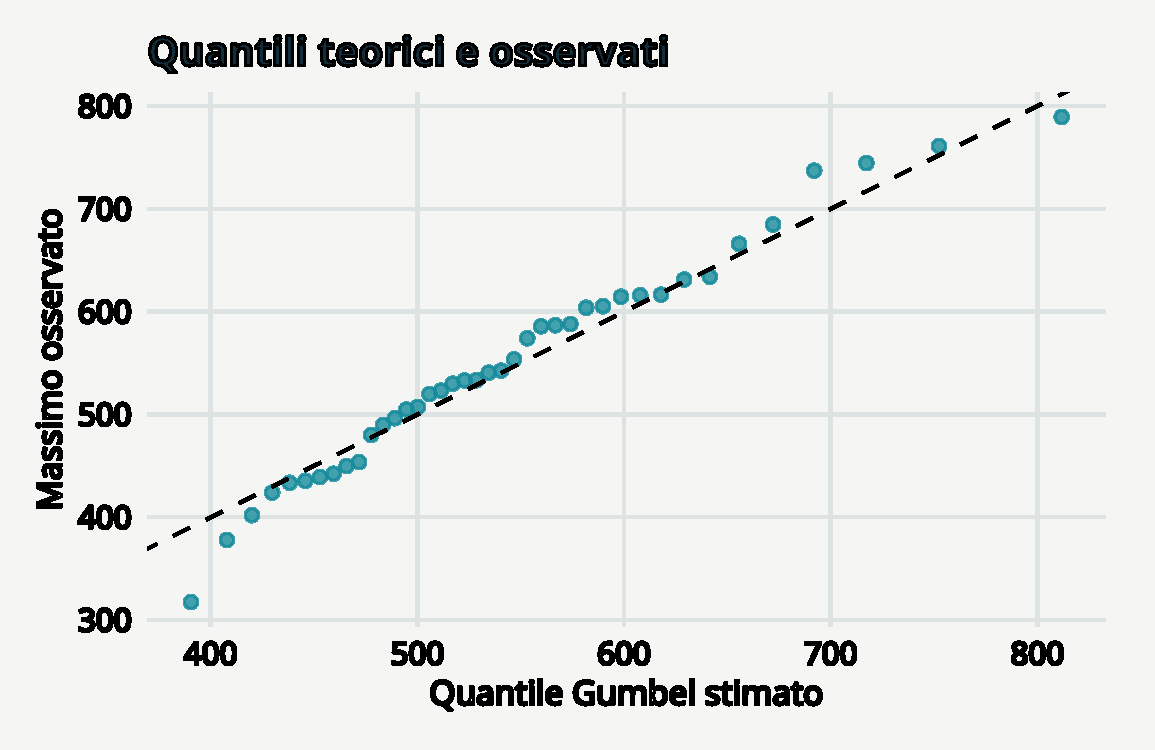
\includegraphics[width=\linewidth,height=6.0cm,keepaspectratio]{Esperimenti/m14-gumbel-A.pdf}\par}
\PSmall{Anni osservati: 40. Seme: 17.}
}};
\node[anchor=north west,inner sep=0] at([xshift=10.85cm,yshift=-2.12cm]current page.north west){\Colonna{8.16cm}{\PLabel{Scenario A · simulazione}
\PBody{La distribuzione Gumbel per massimi descrive una famiglia asimmetrica caratterizzata da posizione e scala positiva. Il programma genera un record sintetico da parametri fissati e li ristima mediante media e deviazione standard campionarie. Il controllo sulla lunghezza del record permette di osservare quanto le stime dipendano dall’informazione disponibile.}
\par\smallskip{\centering\adjustbox{max width=.98\linewidth}{$\displaystyle F(x)=\exp\{-\exp[-(x-\mu)/\beta]\},\quad\beta>0$}\par\smallskip}
\PSmall{$\mu$ è il parametro di posizione e β la scala, che deve essere positiva. F(x) è la probabilità cumulativa dei massimi. La stima ai momenti utilizza $\hat\beta=s\sqrt{6}/\pi$ e $\hat\mu=\bar x-\gamma\hat\beta$, con γ costante di Eulero–Mascheroni.}
}};
\node[anchor=north east,inner sep=0] at([xshift=17.1cm,yshift=-12.04cm]current page.north west){\fontsize{7.7}{9}\selectfont \href{https://marzione00.github.io/Lab_Geo/\#laboratorio/m14-gumbel}{\color{Classical}\bfseries Apri il laboratorio · m14-gumbel}};
\end{tikzpicture}\end{frame}

\begin{frame}[plain]\hypertarget{slide33}{}
\bookmark[level=1,page=33]{Confronto | Adattamento di Gumbel ai massimi}
\begin{tikzpicture}[remember picture,overlay]
\PilotChrome{Confronto | Adattamento di Gumbel ai massimi}{MODELLO GUMBEL E VERIFICA DELL’ADATTAMENTO}{33}{La verifica dell’adattamento deve accompagnare l’estrapolazione alle code.}
\node[anchor=north west,inner sep=0] at([xshift=.96cm,yshift=-2.12cm]current page.north west){\Colonna{9.40cm}{{\centering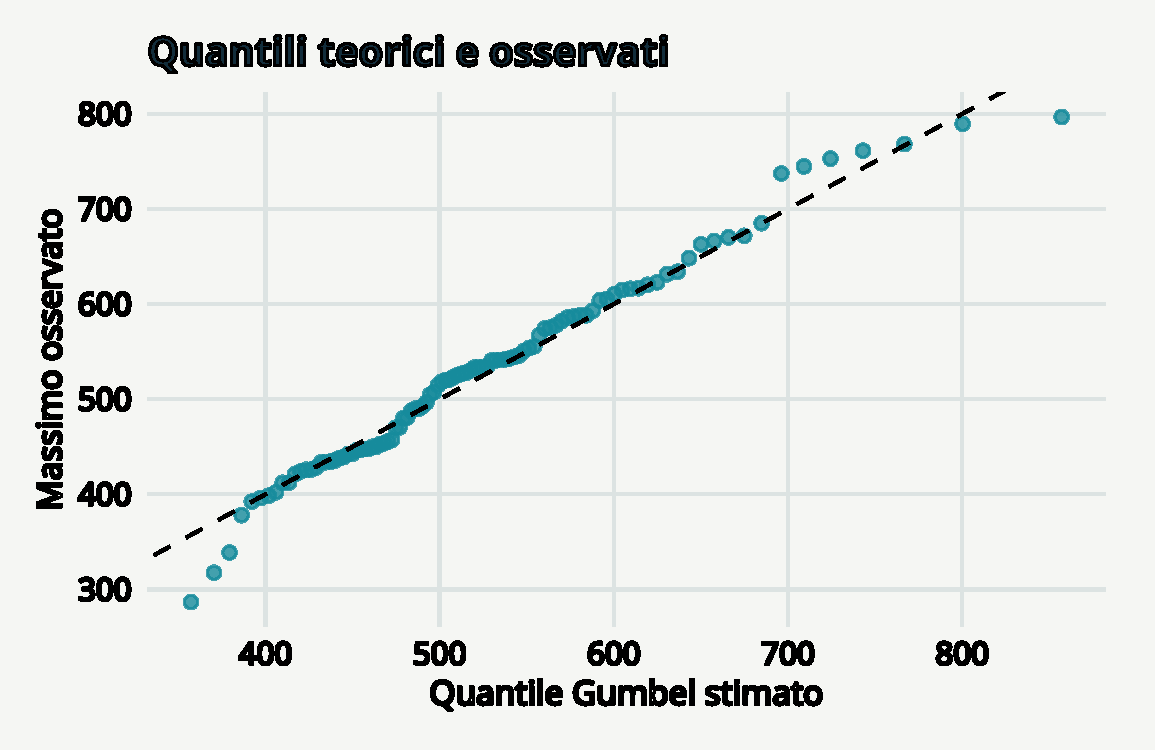
\includegraphics[width=\linewidth,height=5.6cm,keepaspectratio]{Esperimenti/m14-gumbel-B.pdf}\par}
\PSmall{Anni osservati: 40 $\to$ 100. Tutti gli altri parametri e il seme sono fissi.}
}};
\node[anchor=north west,inner sep=0] at([xshift=10.85cm,yshift=-2.12cm]current page.north west){\Colonna{8.16cm}{\PLabel{Confronto fra gli scenari}
{\fontsize{10.2}{12.8}\selectfont\begin{tabular}{@{}>{\raggedright\arraybackslash}p{0.48\linewidth}@{\hspace{.13cm}}>{\raggedright\arraybackslash}p{0.224\linewidth}@{\hspace{.13cm}}>{\raggedright\arraybackslash}p{0.224\linewidth}@{}}\toprule Grandezza & A & B\\[2.3pt]
\midrule 
Posizione stimata & 501 & 482\\[2.3pt]
Scala stimata & 84 & 81,4\\[2.3pt]
Anni osservati & 40 & 100\\[2.3pt]
\bottomrule\end{tabular}\par}
\vspace{.25cm}\PBody{Con 100 anni il modello usa più osservazioni. Le due stime puntuali illustrano una realizzazione per ciascuna lunghezza del record, non una misura generale del bias.}
}};
\node[anchor=north east,inner sep=0] at([xshift=17.1cm,yshift=-12.04cm]current page.north west){\fontsize{7.7}{9}\selectfont \href{https://marzione00.github.io/Lab_Geo/\#laboratorio/m14-gumbel}{\color{Classical}\bfseries Apri il laboratorio · m14-gumbel}};
\end{tikzpicture}\end{frame}

\begin{frame}[plain]\hypertarget{slide34}{}
\bookmark[level=0,page=34]{Livelli rari e incertezza della stima}
\bookmark[level=1,page=34]{Allungare il tempo di ritorno sposta la stima}
\begin{tikzpicture}[remember picture,overlay]
\PilotChrome{Allungare il tempo di ritorno sposta la stima}{LIVELLI RARI E INCERTEZZA DELLA STIMA}{34}{Riporta insieme lunghezza del record, tempo di ritorno e famiglia di distribuzioni.}
\node[anchor=north west,inner sep=0] at([xshift=.96cm,yshift=-2.12cm]current page.north west){\Colonna{9.40cm}{\PLabel{Domanda}
\PBody{Usiamo il medesimo modello con periodi di ritorno di 10, 100 e 500 anni. Il record del corso copre cento massimi annuali sintetici.}
\vspace{.35cm}\PLabel{Interpretazione}
\PBody{Il livello cinquecentennale richiede un’estrapolazione più lunga. La formula restituisce un numero anche quando i dati vincolano debolmente la coda.}
}};
\node[anchor=north west,inner sep=0] at([xshift=10.85cm,yshift=-2.12cm]current page.north west){\Colonna{8.16cm}{\begin{tcolorbox}[enhanced,arc=1.7mm,boxrule=.6pt,colback=white,colframe=Classical!60!Navy,colbacktitle=Navy,coltitle=white,fonttitle=\bfseries\small,title={R · calcolo riproducibile},left=1.7mm,right=1.3mm,top=1.1mm,bottom=1.1mm,before skip=1mm,after skip=1.0mm]\lstinputlisting[style=GeoR,language=R]{Codice/capitolo-04.R}\end{tcolorbox}
\PLabel{Risultato in R}
\begin{tcolorbox}[colback=GeoTint,colframe=Rule,boxrule=.5pt,arc=1.4mm,left=2mm,right=1mm,top=1mm,bottom=1mm]{\fontsize{9}{12}\selectfont\ttfamily \mbox{[1]\ 663.0\ 857.9\ 991.7}}\end{tcolorbox}}};
\end{tikzpicture}\end{frame}

\begin{frame}[plain]\hypertarget{slide35}{}
\bookmark[level=1,page=35]{Livelli di ritorno ed estrapolazione}
\begin{tikzpicture}[remember picture,overlay]
\PilotChrome{Livelli di ritorno ed estrapolazione}{LIVELLI RARI E INCERTEZZA DELLA STIMA}{35}{L’orizzonte di ritorno deve essere confrontato con la durata e con la qualità del record.}
\node[anchor=north west,inner sep=0] at([xshift=.96cm,yshift=-2.12cm]current page.north west){\Colonna{9.40cm}{{\centering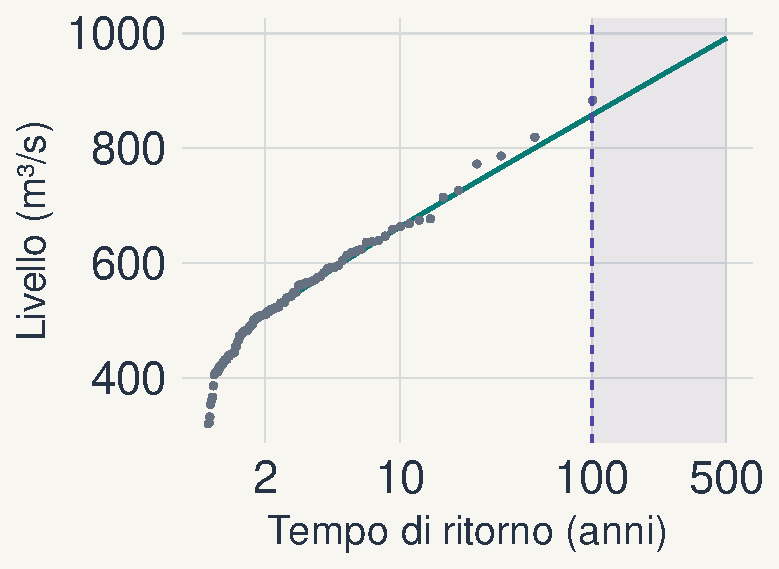
\includegraphics[width=\linewidth,height=6.15cm,keepaspectratio]{Figure/F07.pdf}\par}
\PSmall{a = 476,26 e b = 82,96 m³/s, stimati sul record. Curva Gumbel e punti empirici; fondo viola oltre cento anni.}
}};
\node[anchor=north west,inner sep=0] at([xshift=10.85cm,yshift=-2.12cm]current page.north west){\Colonna{8.16cm}{\PBody{Il livello associato al tempo di ritorno T è il quantile con probabilità cumulativa uno meno uno su T. La Gumbel stimata restituisce circa 857,90 metri cubi al secondo per cento anni e 991,75 per cinquecento anni. Quest’ultimo orizzonte supera la lunghezza del record e rende più forte la dipendenza dalla forma della coda. La curva viene quindi affiancata ai punti empirici e a una regione che segnala i tempi oltre cento anni, affinché l’estrapolazione rimanga visibile.}
\par\smallskip{\centering\adjustbox{max width=.98\linewidth}{$\displaystyle q_T=a-b\log[-\log(1-1/T)],\qquad T>1$}\par\smallskip}
}};
\end{tikzpicture}\end{frame}

\begin{frame}[plain]\hypertarget{slide36}{}
\bookmark[level=1,page=36]{Il ricampionamento ripete l’intera stima}
\begin{tikzpicture}[remember picture,overlay]
\PilotChrome{Il ricampionamento ripete l’intera stima}{LIVELLI RARI E INCERTEZZA DELLA STIMA}{36}{Ogni ripetizione deve comprendere tutti i passaggi di stima che dipendono dal campione.}
\node[anchor=north west,inner sep=0] at([xshift=.96cm,yshift=-2.12cm]current page.north west){\Colonna{9.40cm}{{\centering\resizebox{.97\linewidth}{!}{\begin{tikzpicture}[x=1cm,y=-.87cm,every node/.style={font=\fontsize{12.2}{15}\selectfont,text=Ink},arr/.style={-{Stealth[length=2mm]},line width=.8pt,draw=Classical}]\path[use as bounding box] (0,0) rectangle (7.45,6.2);
\draw[draw=Classical,fill=Classical!8,rounded corners=2pt,line width=.7pt] (0.5,0.6) rectangle (6.9,1.9);
\node[anchor=center,text=Ink,font=\fontsize{12.2}{15}\selectfont,text width=6cm,align=center] at (3.7,1.25) {Campione di cento massimi annuali};
\draw[arr,draw=Classical] (3.7,2.1)--(3.7,2.6);
\draw[draw=Quantum,fill=Quantum!8,rounded corners=2pt,line width=.7pt] (0.5,2.8) rectangle (6.9,4.1);
\node[anchor=center,text=Ink,font=\fontsize{11.5}{15}\selectfont,text width=6cm,align=center] at (3.7,3.45) {Nuovo campione e nuovi $\widehat a,\widehat b$};
\draw[arr,draw=Classical] (3.7,4.3)--(3.7,4.8);
\node[anchor=center,text=Ink,font=\fontsize{15}{15}\selectfont,text width=6cm,align=center] at (3.7,5.4) {Nuovo livello $\widehat q_{100}$};

\end{tikzpicture}}\par}
\PSmall{$\widehat a$: posizione; $\widehat b$: scala; $\widehat q_{100}$: livello centennale. Tutte le stime vengono ricalcolate nel campione estratto.}
}};
\node[anchor=north west,inner sep=0] at([xshift=10.85cm,yshift=-2.12cm]current page.north west){\Colonna{8.16cm}{\PBody{Nel bootstrap dei massimi annuali si estraggono anni con reinserimento e, per ogni campione, si ristimano posizione, scala e livello centennale. Mantenere fissi i parametri durante il ricampionamento escluderebbe proprio la componente di variabilità che si vuole esaminare. Si eseguono 1999 ripetizioni con seme documentato, ricostruendo ogni volta l’intero procedimento di stima. L’interpretazione del bootstrap richiede che gli anni possano essere trattati come unità scambiabili sotto un regime stabile.}
}};
\end{tikzpicture}\end{frame}

\begin{frame}[plain]\hypertarget{slide37}{}
\bookmark[level=1,page=37]{Distribuzione bootstrap del livello centennale}
\begin{tikzpicture}[remember picture,overlay]
\PilotChrome{Distribuzione bootstrap del livello centennale}{LIVELLI RARI E INCERTEZZA DELLA STIMA}{37}{L’incertezza campionaria deve essere distinta dall’incertezza sulla struttura e sulla stabilità del modello.}
\node[anchor=north west,inner sep=0] at([xshift=.96cm,yshift=-2.12cm]current page.north west){\Colonna{9.40cm}{{\centering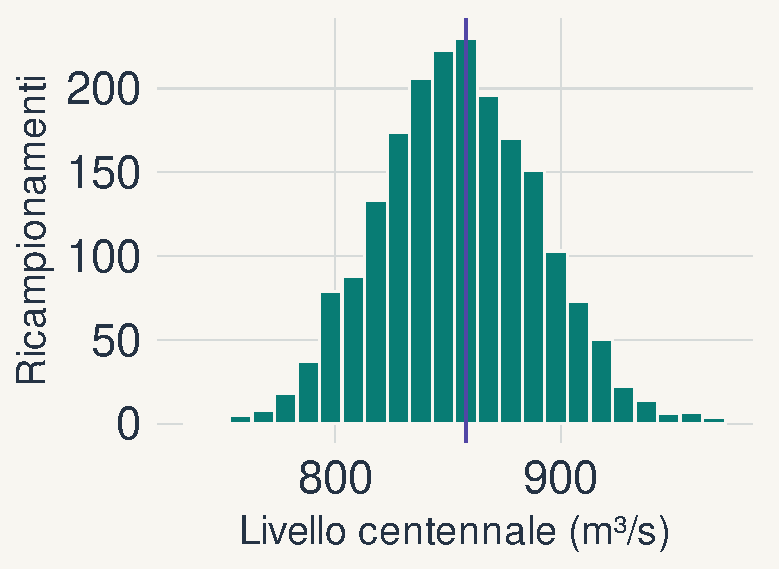
\includegraphics[width=\linewidth,height=6.15cm,keepaspectratio]{Figure/F08.pdf}\par}
\PSmall{1999 stime bootstrap del livello centennale. La linea viola indica la stima sul record completo.}
}};
\node[anchor=north west,inner sep=0] at([xshift=10.85cm,yshift=-2.12cm]current page.north west){\Colonna{8.16cm}{\PBody{I quantili al 2,5\% e 97,5\% della distribuzione bootstrap sono circa 789,16 e 923,10 metri cubi al secondo. L’intervallo percentile descrive la variabilità della procedura sotto le ipotesi di ricampionamento e di modello, senza includere automaticamente cambiamenti futuri del processo o incertezza sulla scelta della famiglia. La dispersione attorno alla stima puntuale rende visibile quanto il livello dipenda dal record finito. Il numero di ripetizioni controlla la precisione Monte Carlo dei quantili e non sostituisce l’informazione osservativa mancante.}
}};
\end{tikzpicture}\end{frame}

\begin{frame}[plain]\hypertarget{slide38}{}
\bookmark[level=1,page=38]{Lunghezza del record e stabilità dei parametri}
\begin{tikzpicture}[remember picture,overlay]
\PilotChrome{Lunghezza del record e stabilità dei parametri}{LIVELLI RARI E INCERTEZZA DELLA STIMA}{38}{La stabilità su campioni annidati è una diagnosi di sensibilità, da interpretare insieme alle ipotesi del modello.}
\node[anchor=north west,inner sep=0] at([xshift=.96cm,yshift=-2.12cm]current page.north west){\Colonna{9.40cm}{{\centering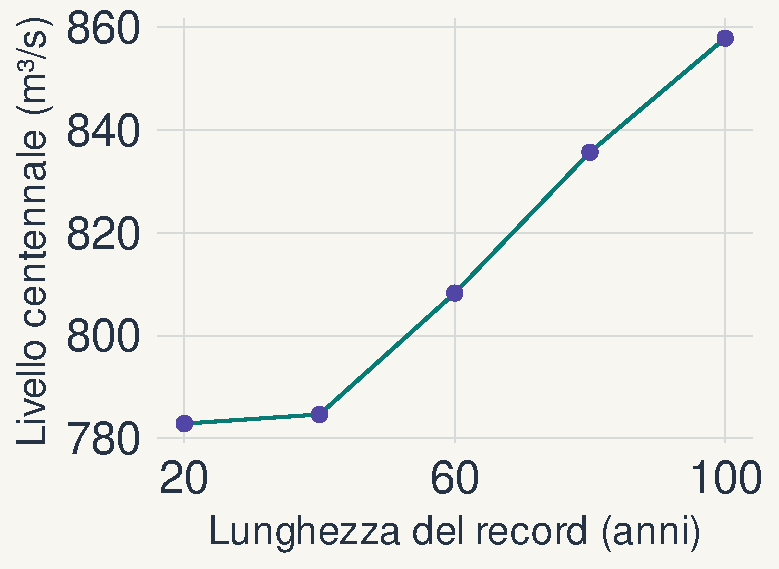
\includegraphics[width=\linewidth,height=6.15cm,keepaspectratio]{Figure/F09.pdf}\par}
\PSmall{Stime su prefissi crescenti dello stesso record sintetico. Il periodo iniziale è comune a tutti i campioni.}
}};
\node[anchor=north west,inner sep=0] at([xshift=10.85cm,yshift=-2.12cm]current page.north west){\Colonna{8.16cm}{\PBody{La stima del livello centennale viene ripetuta utilizzando i primi venti, quaranta, sessanta, ottanta e cento anni. I campioni sono annidati e condividono gran parte delle osservazioni, cosicché i punti della curva non rappresentano esperimenti indipendenti. Le oscillazioni mostrano la sensibilità alla quantità di informazione disponibile e agli estremi progressivamente inclusi. Un tratto apparentemente stabile può essere rassicurante sul campione esaminato, ma non dimostra che il processo resterà invariato né che la famiglia scelta descriva correttamente la coda.}
}};
\end{tikzpicture}\end{frame}

\begin{frame}[plain]\hypertarget{slide39}{}
\bookmark[level=1,page=39]{Influenza del massimo e verifica dell’osservazione}
\begin{tikzpicture}[remember picture,overlay]
\PilotChrome{Influenza del massimo e verifica dell’osservazione}{LIVELLI RARI E INCERTEZZA DELLA STIMA}{39}{L’influenza di un estremo richiede un controllo documentato, senza cancellarne automaticamente l’informazione.}
\node[anchor=north west,inner sep=0] at([xshift=.96cm,yshift=-2.12cm]current page.north west){\Colonna{9.40cm}{{\centering\resizebox{.97\linewidth}{!}{\begin{tikzpicture}[x=1cm,y=-.87cm,every node/.style={font=\fontsize{12.2}{15}\selectfont,text=Ink},arr/.style={-{Stealth[length=2mm]},line width=.8pt,draw=Classical}]\path[use as bounding box] (0,0) rectangle (7.45,6.2);
\draw[draw=Classical,fill=Classical!8,rounded corners=2pt,line width=.7pt] (0.5,1.1) rectangle (3.3,3.5);
\draw[draw=Quantum,fill=Quantum!8,rounded corners=2pt,line width=.7pt] (4.1,1.1) rectangle (6.9,3.5);
\node[anchor=center,text=Ink,font=\fontsize{11}{15}\selectfont,text width=2.5cm,align=center] at (1.9,2.3) {Originale\par857,90 m³/s};
\node[anchor=center,text=Ink,font=\fontsize{11}{15}\selectfont,text width=2.5cm,align=center] at (5.5,2.3) {Massimo +30\%\par897,27 m³/s};
\node[anchor=center,text=Ink,font=\fontsize{11}{15}\selectfont,text width=6.8cm,align=center] at (3.7,4.6) {Livello centennale stimato nei due casi};
\node[anchor=center,text=Ink,font=\fontsize{11}{15}\selectfont,text width=6.8cm,align=center] at (3.7,5.6) {La verifica riguarda l’evento e la sua misura.};

\end{tikzpicture}}\par}
}};
\node[anchor=north west,inner sep=0] at([xshift=10.85cm,yshift=-2.12cm]current page.north west){\Colonna{8.16cm}{\PBody{Aumentando del trenta per cento il massimo in una copia del record, il livello centennale passa da circa 857,90 a 897,27 metri cubi al secondo. Il confronto quantifica l’influenza di un’estremità campionaria sulla stima dei momenti, mantenendo intatti i dati originari. Un valore influente può essere un errore di misura oppure un evento raro pertinente alla coda, per cui l’eliminazione richiede evidenze indipendenti. La relazione dovrebbe documentare il controllo dell’evento e l’effetto delle decisioni alternative sulla conclusione.}
}};
\end{tikzpicture}\end{frame}

\begin{frame}[plain]\hypertarget{slide40}{}
\bookmark[level=1,page=40]{Confronto fra periodi e attribuzione dei cambiamenti}
\begin{tikzpicture}[remember picture,overlay]
\PilotChrome{Confronto fra periodi e attribuzione dei cambiamenti}{LIVELLI RARI E INCERTEZZA DELLA STIMA}{40}{La descrizione di una differenza temporale deve essere separata dall’identificazione del suo meccanismo.}
\node[anchor=north west,inner sep=0] at([xshift=.96cm,yshift=-2.12cm]current page.north west){\Colonna{9.40cm}{\PLabel{Metodo}
\PBody{Le due metà del record comprendono cinquanta anni ciascuna e possono mostrare medie e dispersioni differenti anche quando il processo generatore è costante, come nella simulazione inclusa. Il confronto descrittivo deve precedere ogni attribuzione a cambiamenti climatici, uso del suolo o opere nel bacino. Per dati osservativi, metadati, omogeneità delle misure e ipotesi sulle forzanti sono necessari a distinguere variabilità campionaria e cambiamento del processo. Una suddivisione scelta dopo avere osservato il massimo contrasto introduce inoltre un effetto di selezione.}
}};
\node[anchor=north west,inner sep=0] at([xshift=10.85cm,yshift=-2.12cm]current page.north west){\Colonna{8.16cm}{\PLabel{Formalismo}
\par\smallskip{\centering\adjustbox{max width=.98\linewidth}{$\displaystyle \Delta\overline M=\overline M_{1970:2019}-\overline M_{1920:1969}$}\par\smallskip}
\PLabel{Interpretazione}
\PBody{Un’indagine temporale può includere covariate, modelli non stazionari e controlli di sensibilità, purché la complessità sia sostenuta dall’informazione disponibile. La differenza fra due statistiche descrittive costituisce un punto di partenza per l’analisi, non una spiegazione causale.}
}};
\end{tikzpicture}\end{frame}

\begin{frame}[plain]\hypertarget{slide41}{}
\bookmark[level=1,page=41]{La stima centennale cambia al ricampionamento}
\begin{tikzpicture}[remember picture,overlay]
\PilotChrome{La stima centennale cambia al ricampionamento}{LIVELLI RARI E INCERTEZZA DELLA STIMA}{41}{Le righe sono quantili del risultato bootstrap del laboratorio.}
\node[anchor=north west,inner sep=0] at([xshift=.96cm,yshift=-2.12cm]current page.north west){\Colonna{9.40cm}{\PLabel{Risultati del calcolo in R}
{\fontsize{10.2}{12.8}\selectfont\begin{tabular}{@{}>{\raggedright\arraybackslash}p{0.44\linewidth}@{\hspace{.13cm}}>{\raggedright\arraybackslash}p{0.48\linewidth}@{}}\toprule Probabilità & livello100\\[2.3pt]
\midrule 
0,025 & 784,48\\[2.3pt]
0,5 & 847,31\\[2.3pt]
0,975 & 923,51\\[2.3pt]
\bottomrule\end{tabular}\par}
}};
\node[anchor=north west,inner sep=0] at([xshift=10.85cm,yshift=-2.12cm]current page.north west){\Colonna{8.16cm}{\PBody{Di quanto varia il livello centennale se si ricampionano gli anni e si riadatta ogni volta la distribuzione?}
\vspace{.4cm}\PInfo{Le righe sono quantili del risultato bootstrap del laboratorio. Un nuovo piano di estrazione può produrre estremi leggermente diversi a parità di modello.}
}};
\node[anchor=north east,inner sep=0] at([xshift=17.1cm,yshift=-12.04cm]current page.north west){\fontsize{7.7}{9}\selectfont \href{https://github.com/marzione00/Lab_Geo/blob/649f7cc577b96bd1044d81e78a2f530813e4f96b/materiali/laboratori/M14/M14_N12.R}{\color{Classical}\bfseries Script R · M14\_N12}};
\end{tikzpicture}\end{frame}

\begin{frame}[plain]\hypertarget{slide42}{}
\bookmark[level=1,page=42]{Un singolo massimo influenza la stima di coda}
\begin{tikzpicture}[remember picture,overlay]
\PilotChrome{Un singolo massimo influenza la stima di coda}{LIVELLI RARI E INCERTEZZA DELLA STIMA}{42}{Il massimo modifica media e dispersione e quindi entrambi i parametri Gumbel.}
\node[anchor=north west,inner sep=0] at([xshift=.96cm,yshift=-2.12cm]current page.north west){\Colonna{9.40cm}{\PLabel{Risultati del calcolo in R}
{\fontsize{10.2}{12.8}\selectfont\begin{tabular}{@{}>{\raggedright\arraybackslash}p{0.44\linewidth}@{\hspace{.13cm}}>{\raggedright\arraybackslash}p{0.48\linewidth}@{}}\toprule caso & livello100\\[2.3pt]
\midrule 
originale & 857,9\\[2.3pt]
massimo+30\% & 897,27\\[2.3pt]
\bottomrule\end{tabular}\par}
}};
\node[anchor=north west,inner sep=0] at([xshift=10.85cm,yshift=-2.12cm]current page.north west){\Colonna{8.16cm}{\PBody{Quanto cambia il livello centennale aumentando soltanto il massimo osservato?}
\vspace{.4cm}\PInfo{Il massimo modifica media e dispersione e quindi entrambi i parametri Gumbel. L’esperimento misura sensibilità a una perturbazione dichiarata.}
}};
\node[anchor=north east,inner sep=0] at([xshift=17.1cm,yshift=-12.04cm]current page.north west){\fontsize{7.7}{9}\selectfont \href{https://github.com/marzione00/Lab_Geo/blob/649f7cc577b96bd1044d81e78a2f530813e4f96b/materiali/laboratori/M14/M14_N14.R}{\color{Classical}\bfseries Script R · M14\_N14}};
\end{tikzpicture}\end{frame}

\begin{frame}[plain]\hypertarget{slide43}{}
\bookmark[level=1,page=43]{Livelli di ritorno e incertezza bootstrap}
\begin{tikzpicture}[remember picture,overlay]
\PilotChrome{Livelli di ritorno e incertezza bootstrap}{LIVELLI RARI E INCERTEZZA DELLA STIMA}{43}{Esaminare l’incertezza di un livello raro condizionatamente al modello.}
\node[anchor=north west,inner sep=0] at([xshift=.96cm,yshift=-2.12cm]current page.north west){\Colonna{9.40cm}{{\centering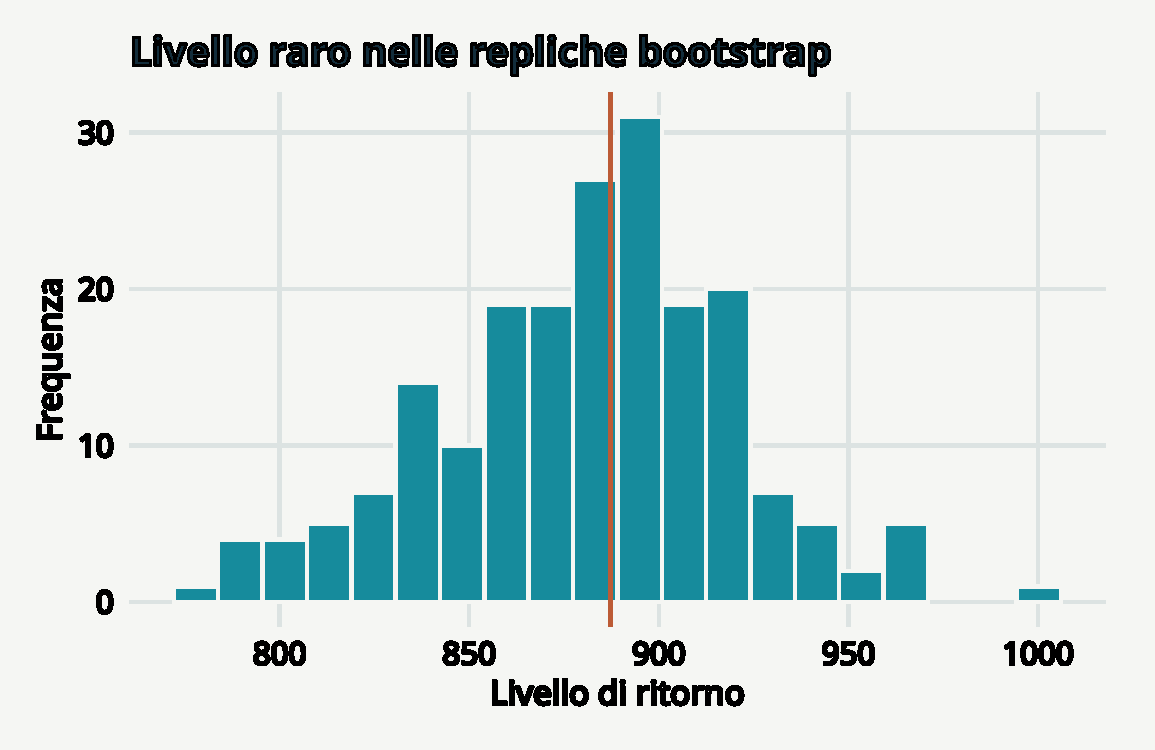
\includegraphics[width=\linewidth,height=6.0cm,keepaspectratio]{Esperimenti/m14-livelli-rari-A.pdf}\par}
\PSmall{Tempo di ritorno [anni]: 100. Seme: 17.}
}};
\node[anchor=north west,inner sep=0] at([xshift=10.85cm,yshift=-2.12cm]current page.north west){\Colonna{8.16cm}{\PLabel{Scenario A · simulazione}
\PBody{Un livello di ritorno è il quantile associato a una probabilità annuale di superamento prefissata. L’esperimento stima una Gumbel da massimi sintetici e ricampiona le osservazioni con reinserimento; in ogni replica ristima posizione, scala e livello richiesto. L’istogramma rappresenta quindi la variabilità del procedimento completo di stima.}
\par\smallskip{\centering\adjustbox{max width=.98\linewidth}{$\displaystyle q_T=\mu-\beta\log[-\log(1-1/T)]$}\par\smallskip}
\PSmall{T è il tempo di ritorno, maggiore di un anno; $q_T$ è il quantile con probabilità cumulativa $1-1/T$. $\mu$ e β sono posizione e scala Gumbel ristimate in ciascun campione bootstrap.}
}};
\node[anchor=north east,inner sep=0] at([xshift=17.1cm,yshift=-12.04cm]current page.north west){\fontsize{7.7}{9}\selectfont \href{https://marzione00.github.io/Lab_Geo/\#laboratorio/m14-livelli-rari}{\color{Classical}\bfseries Apri il laboratorio · m14-livelli-rari}};
\end{tikzpicture}\end{frame}

\begin{frame}[plain]\hypertarget{slide44}{}
\bookmark[level=1,page=44]{Confronto | Livelli di ritorno e incertezza bootstrap}
\begin{tikzpicture}[remember picture,overlay]
\PilotChrome{Confronto | Livelli di ritorno e incertezza bootstrap}{LIVELLI RARI E INCERTEZZA DELLA STIMA}{44}{L’estrapolazione oltre la lunghezza del record aumenta la dipendenza dal modello di coda.}
\node[anchor=north west,inner sep=0] at([xshift=.96cm,yshift=-2.12cm]current page.north west){\Colonna{9.40cm}{{\centering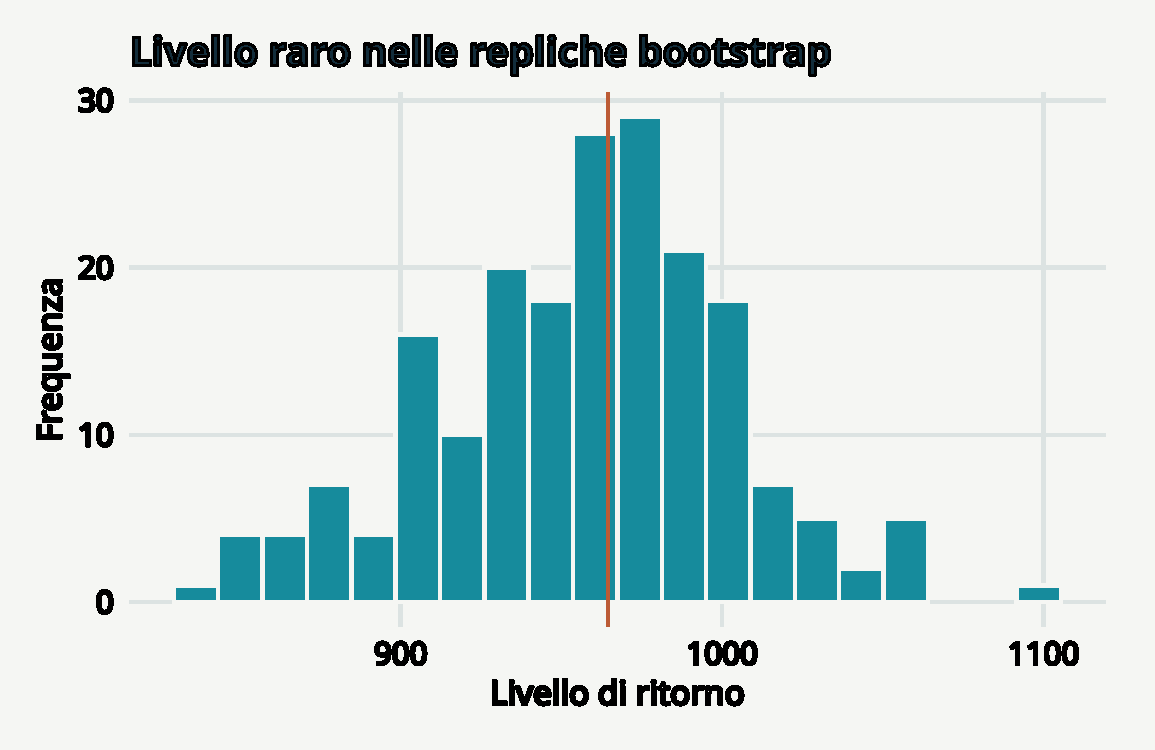
\includegraphics[width=\linewidth,height=5.6cm,keepaspectratio]{Esperimenti/m14-livelli-rari-B.pdf}\par}
\PSmall{Tempo di ritorno [anni]: 100 $\to$ 250. Tutti gli altri parametri e il seme sono fissi.}
}};
\node[anchor=north west,inner sep=0] at([xshift=10.85cm,yshift=-2.12cm]current page.north west){\Colonna{8.16cm}{\PLabel{Confronto fra gli scenari}
{\fontsize{10.2}{12.8}\selectfont\begin{tabular}{@{}>{\raggedright\arraybackslash}p{0.48\linewidth}@{\hspace{.13cm}}>{\raggedright\arraybackslash}p{0.224\linewidth}@{\hspace{.13cm}}>{\raggedright\arraybackslash}p{0.224\linewidth}@{}}\toprule Grandezza & A & B\\[2.3pt]
\midrule 
Livello stimato & 887 & 965\\[2.3pt]
Limite 2,5\%.2.5\% & 798 & 862\\[2.3pt]
Limite 97,5\%.97.5\% & 964 & 1055\\[2.3pt]
T maggiore del record & sì & sì\\[2.3pt]
\bottomrule\end{tabular}\par}
\vspace{.25cm}\PBody{Allungando il ritorno a 250 anni aumentano stima ed estremi dell’intervallo. Il modello viene interrogato più lontano nella coda.}
}};
\node[anchor=north east,inner sep=0] at([xshift=17.1cm,yshift=-12.04cm]current page.north west){\fontsize{7.7}{9}\selectfont \href{https://marzione00.github.io/Lab_Geo/\#laboratorio/m14-livelli-rari}{\color{Classical}\bfseries Apri il laboratorio · m14-livelli-rari}};
\end{tikzpicture}\end{frame}

\begin{frame}[plain]\hypertarget{slide45}{}
\bookmark[level=0,page=45]{Forma della coda e sensibilità GEV}
\bookmark[level=1,page=45]{Il segno della forma cambia la coda}
\begin{tikzpicture}[remember picture,overlay]
\PilotChrome{Il segno della forma cambia la coda}{FORMA DELLA CODA E SENSIBILITÀ GEV}{45}{Nei quantili lontani anche una piccola variazione della forma può pesare molto.}
\node[anchor=north west,inner sep=0] at([xshift=.96cm,yshift=-2.12cm]current page.north west){\Colonna{9.40cm}{\PLabel{Domanda}
\PBody{Per confrontare famiglie GEV teniamo fisse posizione e scala. Usiamo due valori opposti della forma e guardiamo il quantile centennale.}
\vspace{.35cm}\PLabel{Interpretazione}
\PBody{La coda con forma positiva produce il livello superiore. I due valori sono scenari di sensibilità, non stime ottenute adattando i dati.}
}};
\node[anchor=north west,inner sep=0] at([xshift=10.85cm,yshift=-2.12cm]current page.north west){\Colonna{8.16cm}{\begin{tcolorbox}[enhanced,arc=1.7mm,boxrule=.6pt,colback=white,colframe=Classical!60!Navy,colbacktitle=Navy,coltitle=white,fonttitle=\bfseries\small,title={R · calcolo riproducibile},left=1.7mm,right=1.3mm,top=1.1mm,bottom=1.1mm,before skip=1mm,after skip=1.0mm]\lstinputlisting[style=GeoR,language=R]{Codice/capitolo-05.R}\end{tcolorbox}
\PLabel{Risultato in R}
\begin{tcolorbox}[colback=GeoTint,colframe=Rule,boxrule=.5pt,arc=1.4mm,left=2mm,right=1mm,top=1mm,bottom=1mm]{\fontsize{9}{12}\selectfont\ttfamily \mbox{[1]\ \ 751.9\ 1025.9}}\end{tcolorbox}}};
\end{tikzpicture}\end{frame}

\begin{frame}[plain]\hypertarget{slide46}{}
\bookmark[level=1,page=46]{La famiglia generalizzata dei valori estremi}
\begin{tikzpicture}[remember picture,overlay]
\PilotChrome{La famiglia generalizzata dei valori estremi}{FORMA DELLA CODA E SENSIBILITÀ GEV}{46}{Il parametro di forma modifica sia il supporto sia l’estrapolazione della coda.}
\node[anchor=north west,inner sep=0] at([xshift=.96cm,yshift=-2.12cm]current page.north west){\Colonna{9.40cm}{{\centering\resizebox{.97\linewidth}{!}{\begin{tikzpicture}[x=1cm,y=-.87cm,every node/.style={font=\fontsize{12.2}{15}\selectfont,text=Ink},arr/.style={-{Stealth[length=2mm]},line width=.8pt,draw=Classical}]\path[use as bounding box] (0,0) rectangle (7.45,6.2);
\node[anchor=center,text=Ink,font=\fontsize{12.2}{15}\selectfont] at (3.7,0.7) {Tre comportamenti della coda};
\draw[draw=Classical,fill=Classical!8,rounded corners=2pt,line width=.7pt] (0.5,1.7) rectangle (6.9,2.8);
\node[anchor=center,text=Ink,font=\fontsize{12}{15}\selectfont,text width=6cm,align=center] at (3.7,2.25) {$\xi<0$: limite superiore finito};
\draw[draw=Quantum,fill=Quantum!8,rounded corners=2pt,line width=.7pt] (0.5,3) rectangle (6.9,4.1);
\node[anchor=center,text=Ink,font=\fontsize{12}{15}\selectfont,text width=6cm,align=center] at (3.7,3.55) {$\xi=0$: limite Gumbel};
\draw[draw=Measure,fill=Measure!8,rounded corners=2pt,line width=.7pt] (0.5,4.3) rectangle (6.9,5.4);
\node[anchor=center,text=Ink,font=\fontsize{12}{15}\selectfont,text width=6cm,align=center] at (3.7,4.85) {$\xi>0$: coda superiore pesante};

\end{tikzpicture}}\par}
\PSmall{$\mu$: posizione; $\sigma$: scala, entrambe in m³/s; $\xi$: forma adimensionale. Per $\xi\to0$ si usa il limite Gumbel.}
}};
\node[anchor=north west,inner sep=0] at([xshift=10.85cm,yshift=-2.12cm]current page.north west){\Colonna{8.16cm}{\PBody{La GEV aggiunge un parametro di forma xi, che controlla il comportamento della coda oltre a posizione e scala. La distribuzione è definita dove il termine di supporto rimane positivo, mentre il limite per xi tendente a zero restituisce la Gumbel. Una forma positiva produce una coda superiore più pesante; una forma negativa introduce un estremo superiore finito. L’incertezza di xi può influenzare fortemente i livelli con tempi di ritorno lunghi.}
\par\smallskip{\centering\adjustbox{max width=.98\linewidth}{$\displaystyle F(q)=\exp\left\{-\left[1+\xi\frac{q-\mu}{\sigma}\right]^{-1/\xi}\right\}$}\par\smallskip}

\par\smallskip{\centering\adjustbox{max width=.98\linewidth}{$\displaystyle \sigma>0,\qquad1+\xi(q-\mu)/\sigma>0,\qquad\xi\ne0$}\par\smallskip}
}};
\end{tikzpicture}\end{frame}

\begin{frame}[plain]\hypertarget{slide47}{}
\bookmark[level=1,page=47]{Scenari di forma a posizione e scala fissate}
\begin{tikzpicture}[remember picture,overlay]
\PilotChrome{Scenari di forma a posizione e scala fissate}{FORMA DELLA CODA E SENSIBILITÀ GEV}{47}{La sensibilità alla forma deve accompagnare la comunicazione dei livelli molto rari.}
\node[anchor=north west,inner sep=0] at([xshift=.96cm,yshift=-2.12cm]current page.north west){\Colonna{9.40cm}{{\centering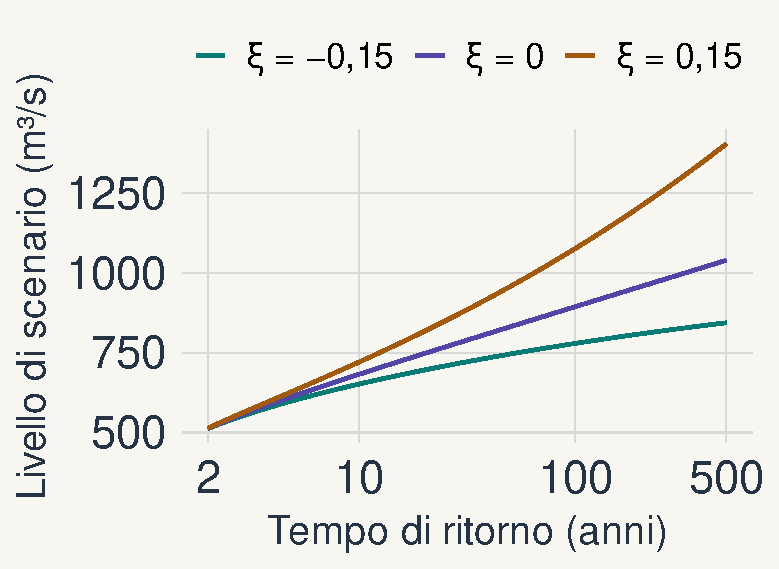
\includegraphics[width=\linewidth,height=6.15cm,keepaspectratio]{Figure/F10.pdf}\par}
\PSmall{$\mu=480$, $\sigma=90$ m³/s; T in anni. Forme prefissate: –0,15, 0, +0,15; per $\xi=0$ si usa il limite Gumbel.}
}};
\node[anchor=north west,inner sep=0] at([xshift=10.85cm,yshift=-2.12cm]current page.north west){\Colonna{8.16cm}{\PBody{Il confronto mantiene posizione pari a 480 e scala pari a 90, variando xi fra meno 0,15, zero e più 0,15. I valori sono ipotesi di sensibilità e non stime aggiuntive dal record. Le curve divergono soprattutto ai tempi di ritorno elevati, rendendo visibile la dipendenza dell’estrapolazione dalla forma della coda. Quando si confrontano implementazioni, occorre verificare anche il segno del parametro: alcune librerie utilizzano una convenzione opposta per la forma, pur rappresentando la stessa famiglia di distribuzioni.}
\par\smallskip{\centering\adjustbox{max width=.98\linewidth}{$\displaystyle q_T=\mu+\frac{\sigma}{\xi}\{[-\log(1-1/T)]^{-\xi}-1\},\quad\xi\ne0$}\par\smallskip}
}};
\end{tikzpicture}\end{frame}

\begin{frame}[plain]\hypertarget{slide48}{}
\bookmark[level=1,page=48]{La scelta della forma pesa di più ai ritorni lunghi}
\begin{tikzpicture}[remember picture,overlay]
\PilotChrome{La scelta della forma pesa di più ai ritorni lunghi}{FORMA DELLA CODA E SENSIBILITÀ GEV}{48}{Confronta i livelli allo stesso tempo di ritorno.}
\node[anchor=north west,inner sep=0] at([xshift=.96cm,yshift=-2.12cm]current page.north west){\Colonna{9.40cm}{\PLabel{Risultati del calcolo in R}
{\fontsize{10.2}{12.8}\selectfont\begin{tabular}{@{}>{\raggedright\arraybackslash}p{0.31\linewidth}@{\hspace{.13cm}}>{\raggedright\arraybackslash}p{0.29\linewidth}@{\hspace{.13cm}}>{\raggedright\arraybackslash}p{0.32\linewidth}@{}}\toprule xi & T & livello\\[2.3pt]
\midrule 
-0,15 & 2 & 512,1\\[2.3pt]
-0,15 & 10 & 651,89\\[2.3pt]
0 & 100 & 894,01\\[2.3pt]
0,15 & 100 & 1076,3\\[2.3pt]
0,15 & 500 & 1403,8\\[2.3pt]
\bottomrule\end{tabular}\par}
\PSmall{Selezione di cinque righe dal file completo.}
}};
\node[anchor=north west,inner sep=0] at([xshift=10.85cm,yshift=-2.12cm]current page.north west){\Colonna{8.16cm}{\PBody{Qual è l’effetto di una forma negativa, nulla o positiva sul livello stimato?}
\vspace{.4cm}\PInfo{Confronta i livelli allo stesso tempo di ritorno. Variare la forma mantenendo posizione e scala fisse isola l’effetto della coda.}
}};
\node[anchor=north east,inner sep=0] at([xshift=17.1cm,yshift=-12.04cm]current page.north west){\fontsize{7.7}{9}\selectfont \href{https://github.com/marzione00/Lab_Geo/blob/649f7cc577b96bd1044d81e78a2f530813e4f96b/materiali/laboratori/M14/M14_N16.R}{\color{Classical}\bfseries Script R · M14\_N16}};
\end{tikzpicture}\end{frame}

\begin{frame}[plain]\hypertarget{slide49}{}
\bookmark[level=1,page=49]{Sensibilità alla forma della coda GEV}
\begin{tikzpicture}[remember picture,overlay]
\PilotChrome{Sensibilità alla forma della coda GEV}{FORMA DELLA CODA E SENSIBILITÀ GEV}{49}{Confrontare livelli rari sotto forme di coda differenti.}
\node[anchor=north west,inner sep=0] at([xshift=.96cm,yshift=-2.12cm]current page.north west){\Colonna{9.40cm}{{\centering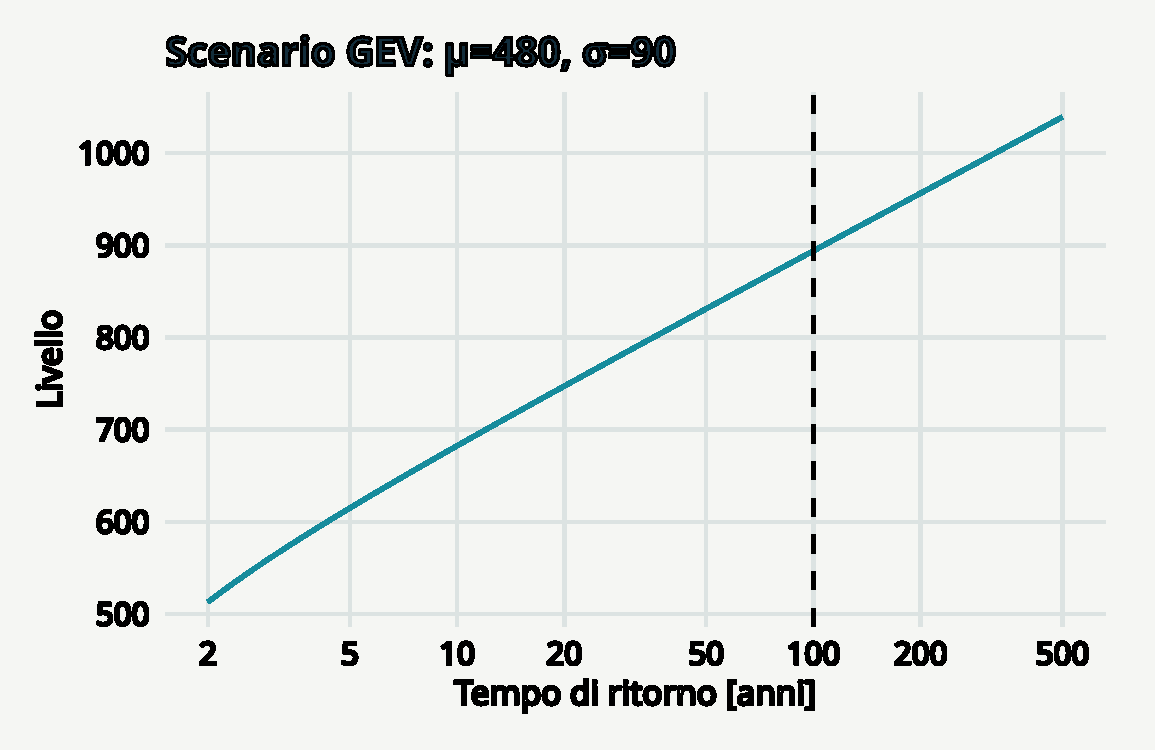
\includegraphics[width=\linewidth,height=6.0cm,keepaspectratio]{Esperimenti/m14-gev-A.pdf}\par}
\PSmall{Parametro di forma $\xi$: 0. Seme: 17.}
}};
\node[anchor=north west,inner sep=0] at([xshift=10.85cm,yshift=-2.12cm]current page.north west){\Colonna{8.16cm}{\PLabel{Scenario A · simulazione}
\PBody{La famiglia generalizzata dei valori estremi introduce un parametro di forma che governa il comportamento della coda. Nell’esperimento, posizione e scala rimangono fissate mentre il controllo modifica la forma, rendendo confrontabili scenari di estrapolazione costruiti sulle medesime grandezze di riferimento. Una linea verticale individua il tempo di ritorno interrogato.}
\par\smallskip{\centering\adjustbox{max width=.98\linewidth}{$\displaystyle q_T=\begin{cases}\mu+\dfrac{\sigma}{\xi}\{[-\log(1-1/T)]^{-\xi}-1\},&\xi\ne0\\\mu-\sigma\log[-\log(1-1/T)],&\xi=0\end{cases}$}\par\smallskip}
\PSmall{$\mu$ è la posizione, $\sigma$ la scala positiva, $\xi$ il parametro di forma e T il tempo di ritorno. Per $\xi<0$ il limite superiore è $\mu-\sigma/\xi$; per $\xi=0$ si usa $q_T=\mu-\sigma\log[-\log(1-1/T)]$.}
}};
\node[anchor=north east,inner sep=0] at([xshift=17.1cm,yshift=-12.04cm]current page.north west){\fontsize{7.7}{9}\selectfont \href{https://marzione00.github.io/Lab_Geo/\#laboratorio/m14-gev}{\color{Classical}\bfseries Apri il laboratorio · m14-gev}};
\end{tikzpicture}\end{frame}

\begin{frame}[plain]\hypertarget{slide50}{}
\bookmark[level=1,page=50]{Confronto | Sensibilità alla forma della coda GEV}
\begin{tikzpicture}[remember picture,overlay]
\PilotChrome{Confronto | Sensibilità alla forma della coda GEV}{FORMA DELLA CODA E SENSIBILITÀ GEV}{50}{Le curve rappresentano scenari di sensibilità e non adattamenti alternativi allo stesso record.}
\node[anchor=north west,inner sep=0] at([xshift=.96cm,yshift=-2.12cm]current page.north west){\Colonna{9.40cm}{{\centering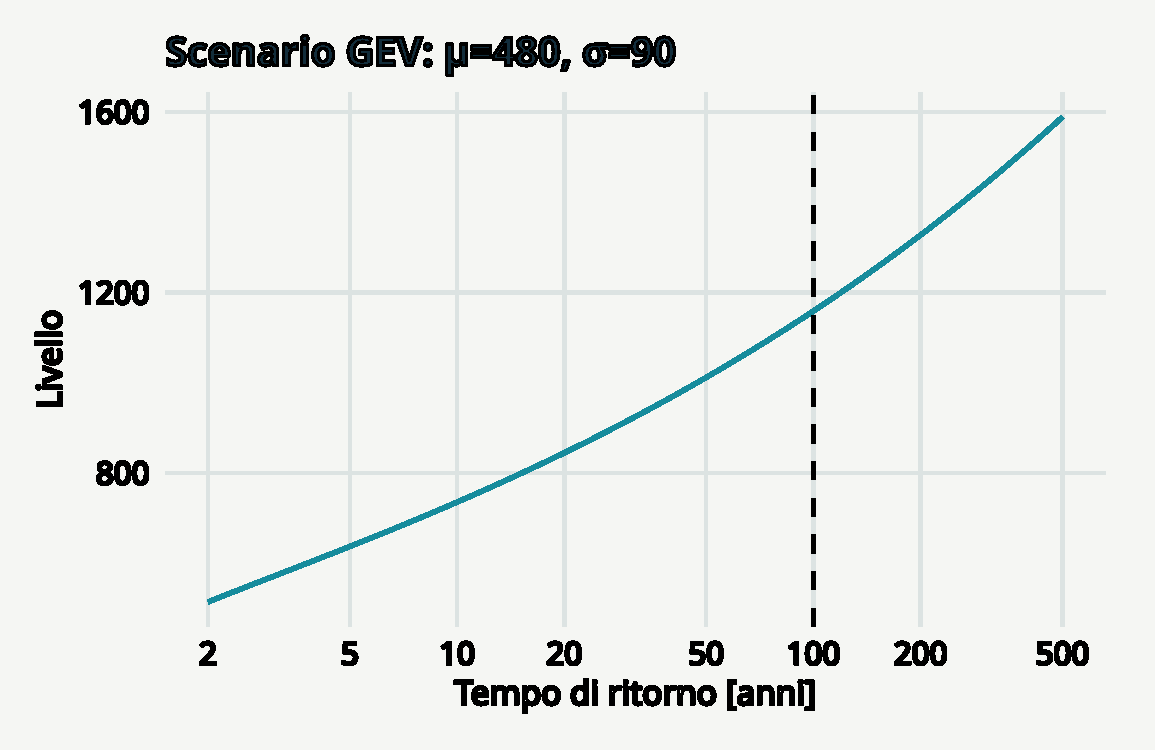
\includegraphics[width=\linewidth,height=5.6cm,keepaspectratio]{Esperimenti/m14-gev-B.pdf}\par}
\PSmall{Parametro di forma $\xi$: 0 $\to$ 0,2. Tutti gli altri parametri e il seme sono fissi.}
}};
\node[anchor=north west,inner sep=0] at([xshift=10.85cm,yshift=-2.12cm]current page.north west){\Colonna{8.16cm}{\PLabel{Confronto fra gli scenari}
{\fontsize{10.2}{12.8}\selectfont\begin{tabular}{@{}>{\raggedright\arraybackslash}p{0.48\linewidth}@{\hspace{.13cm}}>{\raggedright\arraybackslash}p{0.224\linewidth}@{\hspace{.13cm}}>{\raggedright\arraybackslash}p{0.224\linewidth}@{}}\toprule Grandezza & A & B\\[2.3pt]
\midrule 
Livello al T scelto & 894 & 1159\\[2.3pt]
Limite superiore & Non finito & Non finito\\[2.3pt]
Forma $\xi$ & 0 & 0,2\\[2.3pt]
\bottomrule\end{tabular}\par}
\vspace{.25cm}\PBody{Una forma positiva produce una coda più lunga e un livello centennale più alto. Entrambi gli scenari confrontati hanno supporto superiore illimitato.}
}};
\node[anchor=north east,inner sep=0] at([xshift=17.1cm,yshift=-12.04cm]current page.north west){\fontsize{7.7}{9}\selectfont \href{https://marzione00.github.io/Lab_Geo/\#laboratorio/m14-gev}{\color{Classical}\bfseries Apri il laboratorio · m14-gev}};
\end{tikzpicture}\end{frame}

\begin{frame}[plain]\hypertarget{slide51}{}
\bookmark[level=0,page=51]{Superamenti giornalieri ed episodi}
\bookmark[level=1,page=51]{Sei giorni sopra soglia possono formare due episodi}
\begin{tikzpicture}[remember picture,overlay]
\PilotChrome{Sei giorni sopra soglia possono formare due episodi}{SUPERAMENTI GIORNALIERI ED EPISODI}{51}{La regola di separazione deve essere esplicita e coerente con la durata fisica del fenomeno.}
\node[anchor=north west,inner sep=0] at([xshift=.96cm,yshift=-2.12cm]current page.north west){\Colonna{9.40cm}{\PLabel{Domanda}
\PBody{Consideriamo otto giorni consecutivi e una soglia di 10 m³/s. Un episodio comincia al primo giorno oltre soglia dopo un giorno sotto soglia.}
\vspace{.35cm}\PLabel{Interpretazione}
\PBody{Tre giorni consecutivi appartengono allo stesso episodio. Contarli come tre eventi indipendenti cambierebbe la stima della frequenza.}
}};
\node[anchor=north west,inner sep=0] at([xshift=10.85cm,yshift=-2.12cm]current page.north west){\Colonna{8.16cm}{\begin{tcolorbox}[enhanced,arc=1.7mm,boxrule=.6pt,colback=white,colframe=Classical!60!Navy,colbacktitle=Navy,coltitle=white,fonttitle=\bfseries\small,title={R · calcolo riproducibile},left=1.7mm,right=1.3mm,top=1.1mm,bottom=1.1mm,before skip=1mm,after skip=1.0mm]\lstinputlisting[style=GeoR,language=R]{Codice/capitolo-06.R}\end{tcolorbox}
\PLabel{Risultato in R}
\begin{tcolorbox}[colback=GeoTint,colframe=Rule,boxrule=.5pt,arc=1.4mm,left=2mm,right=1mm,top=1mm,bottom=1mm]{\fontsize{9}{12}\selectfont\ttfamily \mbox{giorni\ episodi\ }\\\mbox{\ \ \ \ \ \ 6\ \ \ \ \ \ \ 2}}\end{tcolorbox}}};
\end{tikzpicture}\end{frame}

\begin{frame}[plain]\hypertarget{slide52}{}
\bookmark[level=1,page=52]{Giorni sopra soglia e numero degli episodi}
\begin{tikzpicture}[remember picture,overlay]
\PilotChrome{Giorni sopra soglia e numero degli episodi}{SUPERAMENTI GIORNALIERI ED EPISODI}{52}{La definizione operativa di evento deve precedere il conteggio e il modello probabilistico.}
\node[anchor=north west,inner sep=0] at([xshift=.96cm,yshift=-2.12cm]current page.north west){\Colonna{9.40cm}{{\centering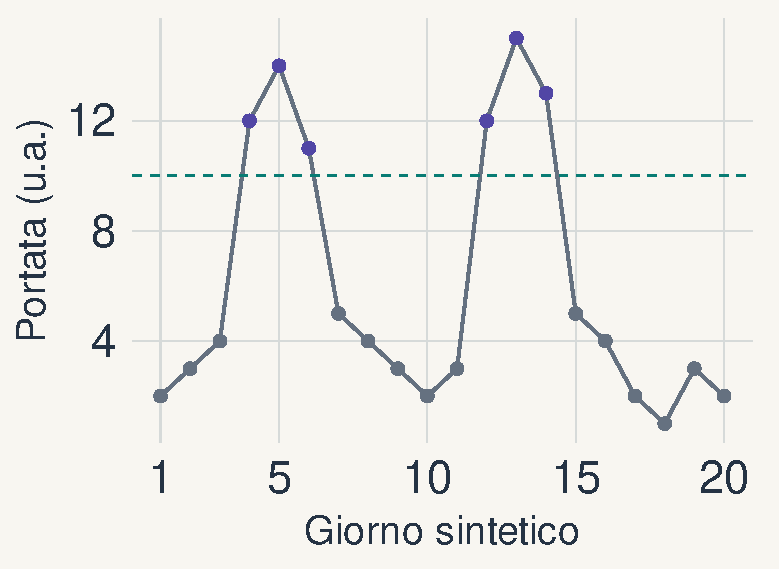
\includegraphics[width=\linewidth,height=6.15cm,keepaspectratio]{Figure/F11.pdf}\par}
\PSmall{Soglia u = 10 nelle unità arbitrarie della serie. I sei punti viola appartengono a due sequenze.}
}};
\node[anchor=north west,inner sep=0] at([xshift=10.85cm,yshift=-2.12cm]current page.north west){\Colonna{8.16cm}{\PBody{La breve serie giornaliera sintetica contiene sei valori superiori alla soglia dieci, organizzati in due sequenze consecutive. Contare i giorni misura la durata discreta del superamento, mentre contare le sequenze individua episodi secondo una regola temporale. Entrambe le quantità possono essere utili, ma rispondono a domande differenti. La distinzione diventa essenziale quando un modello per eventi richiede approssimativa indipendenza: più giorni della stessa piena non costituiscono automaticamente più episodi indipendenti.}
\par\smallskip{\centering\adjustbox{max width=.98\linewidth}{$\displaystyle N_{\rm giorni}=\sum_t\mathbf1\{Q_t>u\}=6$}\par\smallskip}
}};
\end{tikzpicture}\end{frame}

\begin{frame}[plain]\hypertarget{slide53}{}
\bookmark[level=1,page=53]{Separazione delle sequenze e picchi di evento}
\begin{tikzpicture}[remember picture,overlay]
\PilotChrome{Separazione delle sequenze e picchi di evento}{SUPERAMENTI GIORNALIERI ED EPISODI}{53}{La separazione degli episodi deve riflettere la scala di dipendenza del processo.}
\node[anchor=north west,inner sep=0] at([xshift=.96cm,yshift=-2.12cm]current page.north west){\Colonna{9.40cm}{\begin{tcolorbox}[enhanced,arc=1.7mm,boxrule=.6pt,colback=white,colframe=Classical!60!Navy,colbacktitle=Navy,coltitle=white,fonttitle=\bfseries\small,title={R · procedura},left=1.7mm,right=1.3mm,top=1.1mm,bottom=1.1mm,before skip=1mm,after skip=1.0mm]\lstinputlisting[style=GeoR,language=R]{Codice/lettura-27.R}\end{tcolorbox}
}};
\node[anchor=north west,inner sep=0] at([xshift=10.85cm,yshift=-2.12cm]current page.north west){\Colonna{8.16cm}{\PBody{La regola didattica apre un episodio quando un giorno sopra soglia segue un giorno che non la supera, quindi assegna lo stesso gruppo ai superamenti consecutivi. Di ogni gruppo si conserva il massimo, ottenendo picchi pari a quattordici e quindici. Un’analisi idrologica reale può richiedere una separazione minima più lunga e criteri fondati sulla dinamica del bacino. La regola deve essere scelta prima della stima degli estremi, poiché modifica frequenza degli eventi, distribuzione dei picchi e interpretazione dei tempi di ritorno.}
}};
\end{tikzpicture}\end{frame}

\begin{frame}[plain]\hypertarget{slide54}{}
\bookmark[level=1,page=54]{Due strategie per costruire il campione degli estremi}
\begin{tikzpicture}[remember picture,overlay]
\PilotChrome{Due strategie per costruire il campione degli estremi}{SUPERAMENTI GIORNALIERI ED EPISODI}{54}{La scelta del campione degli estremi precede quella della distribuzione da adattare.}
\node[anchor=north west,inner sep=0] at([xshift=.96cm,yshift=-2.12cm]current page.north west){\Colonna{9.40cm}{{\centering\resizebox{.97\linewidth}{!}{\begin{tikzpicture}[x=1cm,y=-.87cm,every node/.style={font=\fontsize{12.2}{15}\selectfont,text=Ink},arr/.style={-{Stealth[length=2mm]},line width=.8pt,draw=Classical}]\path[use as bounding box] (0,0) rectangle (7.45,6.2);
\draw[draw=Classical,fill=Classical!8,rounded corners=2pt,line width=.7pt] (0.5,0.8) rectangle (6.9,2);
\node[anchor=center,text=Ink,font=\fontsize{11}{15}\selectfont,text width=6cm,align=center] at (3.7,1.4) {Serie osservata con risoluzione dichiarata};
\draw[arr,draw=Classical] (2.1,2.2)--(2.1,3.1);
\draw[arr,draw=Quantum] (5.3,2.2)--(5.3,3.1);
\draw[draw=Classical,fill=Classical!8,rounded corners=2pt,line width=.7pt] (0.5,3.3) rectangle (3.5,5.2);
\draw[draw=Quantum,fill=Quantum!8,rounded corners=2pt,line width=.7pt] (3.9,3.3) rectangle (6.9,5.2);
\node[anchor=center,text=Ink,font=\fontsize{12.2}{15}\selectfont,text width=2.6cm,align=center] at (2,4.25) {Massimo\par per blocco};
\node[anchor=center,text=Ink,font=\fontsize{12.2}{15}\selectfont,text width=2.6cm,align=center] at (5.4,4.25) {Picchi\par sopra soglia};
\node[anchor=center,text=Ink,font=\fontsize{11}{15}\selectfont,text width=6.8cm,align=center] at (3.7,5.9) {Campioni costruiti mediante regole differenti.};

\end{tikzpicture}}\par}
}};
\node[anchor=north west,inner sep=0] at([xshift=10.85cm,yshift=-2.12cm]current page.north west){\Colonna{8.16cm}{\PBody{Il metodo dei massimi di blocco conserva un solo valore per intervallo temporale, mentre il metodo dei superamenti di soglia seleziona episodi eccedenti un livello prefissato. Il secondo richiede di definire soglia, separazione degli episodi e frequenza di occorrenza, potendo conservare più informazione sugli eventi rari. I due approcci non condividono automaticamente la stessa numerosità né la stessa interpretazione temporale. Il corso usa i massimi annuali per la stima Gumbel e introduce i superamenti giornalieri per chiarire la costruzione del campione.}
}};
\end{tikzpicture}\end{frame}

\begin{frame}[plain]\hypertarget{slide55}{}
\bookmark[level=1,page=55]{Un picco rappresenta ciascuna sequenza consecutiva}
\begin{tikzpicture}[remember picture,overlay]
\PilotChrome{Un picco rappresenta ciascuna sequenza consecutiva}{SUPERAMENTI GIORNALIERI ED EPISODI}{55}{Il massimo del gruppo sintetizza l’intensità dell’episodio.}
\node[anchor=north west,inner sep=0] at([xshift=.96cm,yshift=-2.12cm]current page.north west){\Colonna{9.40cm}{\PLabel{Risultati del calcolo in R}
{\fontsize{10.2}{12.8}\selectfont\begin{tabular}{@{}>{\raggedright\arraybackslash}p{0.44\linewidth}@{\hspace{.13cm}}>{\raggedright\arraybackslash}p{0.48\linewidth}@{}}\toprule gr & Quantile o portata\\[2.3pt]
\midrule 
1 & 14\\[2.3pt]
2 & 15\\[2.3pt]
\bottomrule\end{tabular}\par}
}};
\node[anchor=north west,inner sep=0] at([xshift=10.85cm,yshift=-2.12cm]current page.north west){\Colonna{8.16cm}{\PBody{Quale portata si conserva da ciascun gruppo di giorni sopra soglia?}
\vspace{.4cm}\PInfo{Il massimo del gruppo sintetizza l’intensità dell’episodio. Per valutare la frequenza occorrono anche durata osservata e regola di separazione.}
}};
\node[anchor=north east,inner sep=0] at([xshift=17.1cm,yshift=-12.04cm]current page.north west){\fontsize{7.7}{9}\selectfont \href{https://github.com/marzione00/Lab_Geo/blob/649f7cc577b96bd1044d81e78a2f530813e4f96b/materiali/laboratori/M14/M14_N18.R}{\color{Classical}\bfseries Script R · M14\_N18}};
\end{tikzpicture}\end{frame}

\begin{frame}[plain]\hypertarget{slide56}{}
\bookmark[level=1,page=56]{Superamenti e separazione degli episodi}
\begin{tikzpicture}[remember picture,overlay]
\PilotChrome{Superamenti e separazione degli episodi}{SUPERAMENTI GIORNALIERI ED EPISODI}{56}{Distinguere giorni sopra soglia ed eventi temporali.}
\node[anchor=north west,inner sep=0] at([xshift=.96cm,yshift=-2.12cm]current page.north west){\Colonna{9.40cm}{{\centering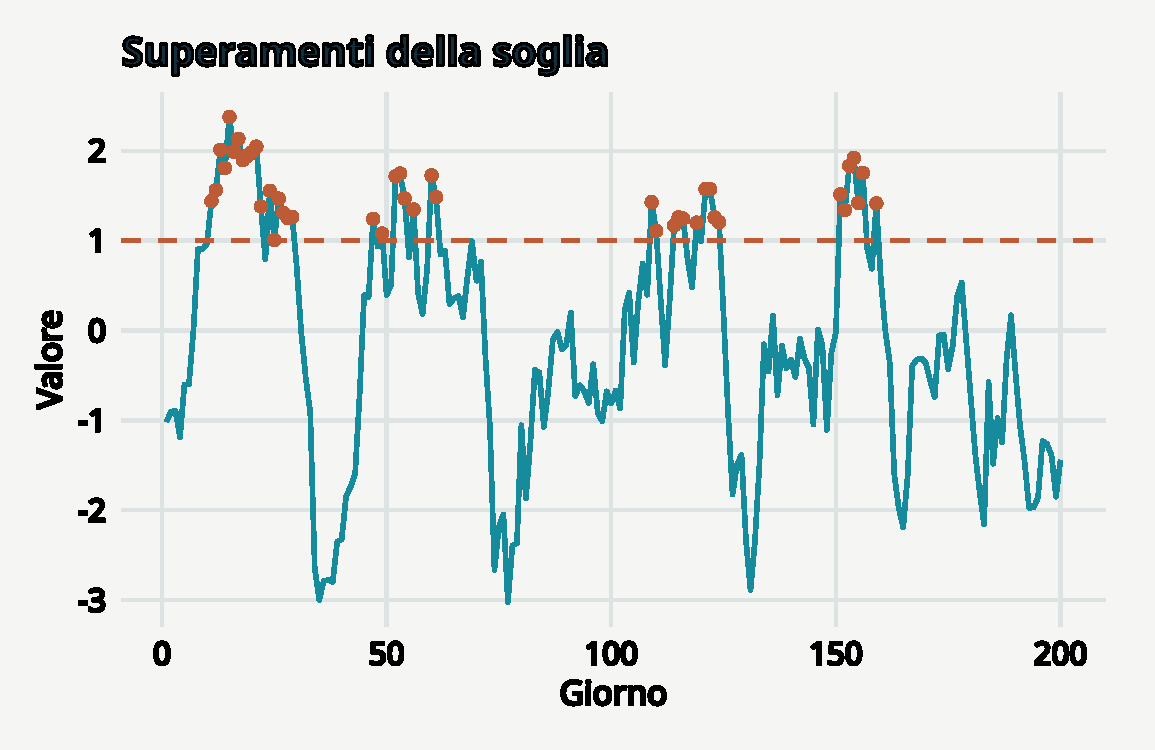
\includegraphics[width=\linewidth,height=6.0cm,keepaspectratio]{Esperimenti/m14-episodi-A.pdf}\par}
\PSmall{Separazione minima [giorni]: 3. Seme: 17.}
}};
\node[anchor=north west,inner sep=0] at([xshift=10.85cm,yshift=-2.12cm]current page.north west){\Colonna{8.16cm}{\PLabel{Scenario A · simulazione}
\PBody{Più giorni sopra soglia possono appartenere allo stesso episodio quando la serie presenta persistenza. Il programma simula un processo autoregressivo stazionario e individua i giorni nei quali il valore supera la soglia scelta. Successivamente raggruppa i superamenti secondo la distanza temporale fra due giorni consecutivi della sequenza selezionata.}
\par\smallskip{\centering\adjustbox{max width=.98\linewidth}{$\displaystyle N_{episodi}=\begin{cases}0,&k=0\\1+\sum_{j=2}^k\mathbf1(t_j-t_{j-1}>r),&k>0\end{cases}$}\par\smallskip}
\PSmall{$t_j$ è il giorno del j-esimo superamento e k il numero totale di giorni selezionati. r è la soglia sulla distanza temporale fra superamenti: una differenza maggiore di r apre un nuovo episodio; per k=0 gli episodi sono zero.}
}};
\node[anchor=north east,inner sep=0] at([xshift=17.1cm,yshift=-12.04cm]current page.north west){\fontsize{7.7}{9}\selectfont \href{https://marzione00.github.io/Lab_Geo/\#laboratorio/m14-episodi}{\color{Classical}\bfseries Apri il laboratorio · m14-episodi}};
\end{tikzpicture}\end{frame}

\begin{frame}[plain]\hypertarget{slide57}{}
\bookmark[level=1,page=57]{Confronto | Superamenti e separazione degli episodi}
\begin{tikzpicture}[remember picture,overlay]
\PilotChrome{Confronto | Superamenti e separazione degli episodi}{SUPERAMENTI GIORNALIERI ED EPISODI}{57}{La definizione di episodio appartiene al modello operativo dell’evento.}
\node[anchor=north west,inner sep=0] at([xshift=.96cm,yshift=-2.12cm]current page.north west){\Colonna{9.40cm}{{\centering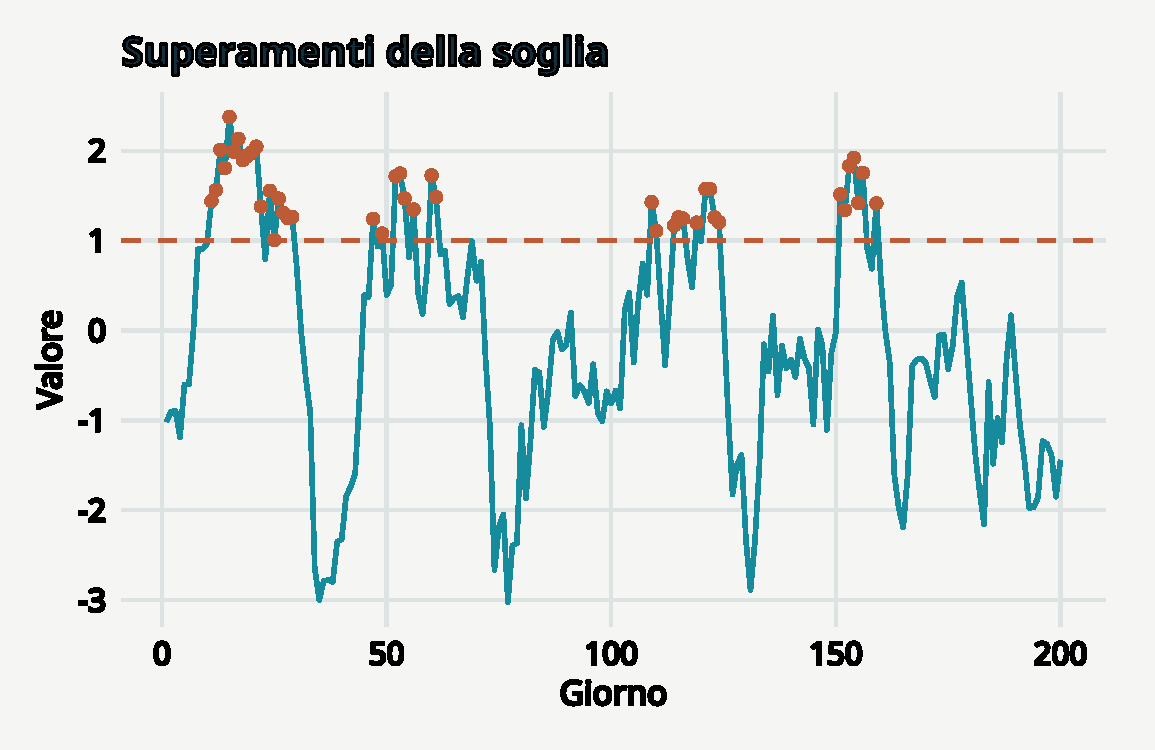
\includegraphics[width=\linewidth,height=5.6cm,keepaspectratio]{Esperimenti/m14-episodi-B.pdf}\par}
\PSmall{Separazione minima [giorni]: 3 $\to$ 6. Tutti gli altri parametri e il seme sono fissi.}
}};
\node[anchor=north west,inner sep=0] at([xshift=10.85cm,yshift=-2.12cm]current page.north west){\Colonna{8.16cm}{\PLabel{Confronto fra gli scenari}
{\fontsize{10.2}{12.8}\selectfont\begin{tabular}{@{}>{\raggedright\arraybackslash}p{0.48\linewidth}@{\hspace{.13cm}}>{\raggedright\arraybackslash}p{0.224\linewidth}@{\hspace{.13cm}}>{\raggedright\arraybackslash}p{0.224\linewidth}@{}}\toprule Grandezza & A & B\\[2.3pt]
\midrule 
Giorni sopra soglia & 43 & 43\\[2.3pt]
Episodi & 6 & 4\\[2.3pt]
Separazione adottata & 3 & 6\\[2.3pt]
\bottomrule\end{tabular}\par}
\vspace{.25cm}\PBody{La soglia individua sempre 43 giorni. Aumentare la separazione minima riunisce alcune sequenze, facendo scendere da sei a quattro il numero di episodi.}
}};
\node[anchor=north east,inner sep=0] at([xshift=17.1cm,yshift=-12.04cm]current page.north west){\fontsize{7.7}{9}\selectfont \href{https://marzione00.github.io/Lab_Geo/\#laboratorio/m14-episodi}{\color{Classical}\bfseries Apri il laboratorio · m14-episodi}};
\end{tikzpicture}\end{frame}

\begin{frame}[plain]\hypertarget{slide58}{}
\bookmark[level=0,page=58]{Pericolosità, conseguenze e comunicazione}
\bookmark[level=1,page=58]{Un cambiamento dell’esposizione modifica la perdita}
\begin{tikzpicture}[remember picture,overlay]
\PilotChrome{Un cambiamento dell’esposizione modifica la perdita}{PERICOLOSITÀ, CONSEGUENZE E COMUNICAZIONE}{58}{La pericolosità descrive il fenomeno; il rischio richiede un modello delle conseguenze.}
\node[anchor=north west,inner sep=0] at([xshift=.96cm,yshift=-2.12cm]current page.north west){\Colonna{9.40cm}{\PLabel{Domanda}
\PBody{In tre classi disgiunte di evento fissiamo probabilità annue e danni ipotetici. Raddoppiamo il valore esposto a parità di pericolosità.}
\vspace{.35cm}\PLabel{Interpretazione}
\PBody{La somma dei prodotti probabilità per danno raddoppia. L’esempio isola l’esposizione e assume proporzionalità dei danni.}
}};
\node[anchor=north west,inner sep=0] at([xshift=10.85cm,yshift=-2.12cm]current page.north west){\Colonna{8.16cm}{\begin{tcolorbox}[enhanced,arc=1.7mm,boxrule=.6pt,colback=white,colframe=Classical!60!Navy,colbacktitle=Navy,coltitle=white,fonttitle=\bfseries\small,title={R · calcolo riproducibile},left=1.7mm,right=1.3mm,top=1.1mm,bottom=1.1mm,before skip=1mm,after skip=1.0mm]\lstinputlisting[style=GeoR,language=R]{Codice/capitolo-07.R}\end{tcolorbox}
\PLabel{Risultato in R}
\begin{tcolorbox}[colback=GeoTint,colframe=Rule,boxrule=.5pt,arc=1.4mm,left=2mm,right=1mm,top=1mm,bottom=1mm]{\fontsize{9}{12}\selectfont\ttfamily \mbox{base\ doppio\ }\\\mbox{\ \ 7300\ \ 14600}}\end{tcolorbox}}};
\end{tikzpicture}\end{frame}

\begin{frame}[plain]\hypertarget{slide59}{}
\bookmark[level=1,page=59]{Pericolosità, esposizione e conseguenze}
\begin{tikzpicture}[remember picture,overlay]
\PilotChrome{Pericolosità, esposizione e conseguenze}{PERICOLOSITÀ, CONSEGUENZE E COMUNICAZIONE}{59}{La probabilità di un evento deve essere collegata a un modello esplicito delle sue conseguenze.}
\node[anchor=north west,inner sep=0] at([xshift=.96cm,yshift=-2.12cm]current page.north west){\Colonna{9.40cm}{{\centering\resizebox{.97\linewidth}{!}{\begin{tikzpicture}[x=1cm,y=-.87cm,every node/.style={font=\fontsize{12.2}{15}\selectfont,text=Ink},arr/.style={-{Stealth[length=2mm]},line width=.8pt,draw=Classical}]\path[use as bounding box] (0,0) rectangle (7.45,6.2);
\draw[draw=Classical,fill=Classical!8,rounded corners=2pt,line width=.7pt] (0.5,0.7) rectangle (6.9,2);
\node[anchor=center,text=Ink,font=\fontsize{11.5}{15}\selectfont,text width=6cm,align=center] at (3.7,1.35) {Probabilità e intensità del fenomeno};
\draw[arr,draw=Classical] (3.7,2.2)--(3.7,2.7);
\draw[draw=Quantum,fill=Quantum!8,rounded corners=2pt,line width=.7pt] (0.5,2.9) rectangle (6.9,4.2);
\node[anchor=center,text=Ink,font=\fontsize{12.2}{15}\selectfont,text width=6cm,align=center] at (3.7,3.55) {Esposizione e vulnerabilità};
\draw[arr,draw=Classical] (3.7,4.4)--(3.7,4.9);
\node[anchor=center,text=Ink,font=\fontsize{12.2}{15}\selectfont,text width=6.7cm,align=center] at (3.7,5.5) {Distribuzione delle conseguenze};

\end{tikzpicture}}\par}
}};
\node[anchor=north west,inner sep=0] at([xshift=10.85cm,yshift=-2.12cm]current page.north west){\Colonna{8.16cm}{\PBody{La pericolosità descrive la probabilità e l’intensità del fenomeno, mentre le conseguenze dipendono da ciò che è esposto e dalla sua vulnerabilità. Un identico livello di piena può quindi produrre perdite differenti in territori con beni, persone e protezioni diversi. Nel caso didattico vengono assegnati danni ipotetici a classi di evento mutuamente esclusive, rendendo esplicito il passaggio dalla probabilità alla perdita. Il risultato è uno scenario numerico e non una valutazione utilizzabile per un’opera o per un sito reale.}
}};
\end{tikzpicture}\end{frame}

\begin{frame}[plain]\hypertarget{slide60}{}
\bookmark[level=1,page=60]{Perdita attesa su classi mutuamente esclusive}
\begin{tikzpicture}[remember picture,overlay]
\PilotChrome{Perdita attesa su classi mutuamente esclusive}{PERICOLOSITÀ, CONSEGUENZE E COMUNICAZIONE}{60}{La somma dei contributi richiede classi compatibili con la definizione probabilistica della perdita.}
\node[anchor=north west,inner sep=0] at([xshift=.96cm,yshift=-2.12cm]current page.north west){\Colonna{9.40cm}{{\centering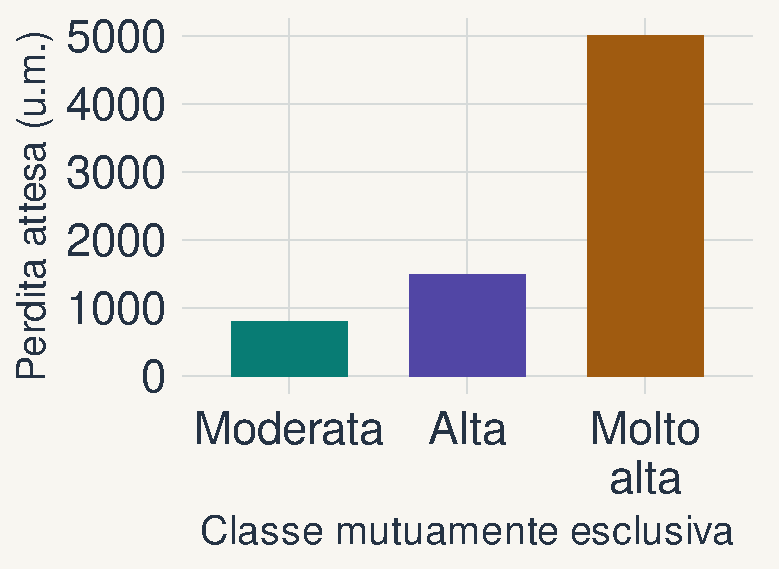
\includegraphics[width=\linewidth,height=6.15cm,keepaspectratio]{Figure/F12.pdf}\par}
\PSmall{L: perdita annua; $p_k$: probabilità della classe k; $\ell_k$: danno. Contributi di classi esclusive; probabilità e danni ipotetici.}
}};
\node[anchor=north west,inner sep=0] at([xshift=10.85cm,yshift=-2.12cm]current page.north west){\Colonna{8.16cm}{\PBody{Le tre classi hanno probabilità annue pari a 0,08, 0,015 e 0,005, con danni ipotetici di diecimila, centomila e un milione di unità monetarie. Il restante novanta per cento viene associato a danno nullo nello scenario. I contributi attesi sono rispettivamente 800, 1500 e 5000, per un totale di 7300 unità monetarie per anno. La classe meno frequente fornisce il contributo maggiore a causa del danno assegnato. Usare probabilità cumulative sovrapposte al posto di classi esclusive conterebbe più volte parte degli eventi.}
\par\smallskip{\centering\adjustbox{max width=.98\linewidth}{$\displaystyle E[L]=\sum_k p_k\ell_k=7300\quad\text{unità monetarie/anno}$}\par\smallskip}
}};
\end{tikzpicture}\end{frame}

\begin{frame}[plain]\hypertarget{slide61}{}
\bookmark[level=1,page=61]{Relazione finale e percorso di laboratorio}
\begin{tikzpicture}[remember picture,overlay]
\PilotChrome{Relazione finale e percorso di laboratorio}{PERICOLOSITÀ, CONSEGUENZE E COMUNICAZIONE}{61}{La comunicazione di un livello raro deve rendere riconoscibili evidenza, incertezza e condizioni di validità.}
\node[anchor=north west,inner sep=0] at([xshift=.96cm,yshift=-2.12cm]current page.north west){\Colonna{9.40cm}{{\centering\resizebox{.97\linewidth}{!}{\begin{tikzpicture}[x=1cm,y=-.87cm,every node/.style={font=\fontsize{12.2}{15}\selectfont,text=Ink},arr/.style={-{Stealth[length=2mm]},line width=.8pt,draw=Classical}]\path[use as bounding box] (0,0) rectangle (7.45,6.2);
\draw[draw=Classical,fill=Classical!8,rounded corners=2pt,line width=.7pt] (0.5,0.6) rectangle (6.9,1.9);
\node[anchor=center,text=Ink,font=\fontsize{12.2}{15}\selectfont,text width=6cm,align=center] at (3.7,1.25) {Record e definizione dell’estremo};
\draw[arr,draw=Classical] (3.7,2.1)--(3.7,2.6);
\draw[draw=Quantum,fill=Quantum!8,rounded corners=2pt,line width=.7pt] (0.5,2.8) rectangle (6.9,4.1);
\node[anchor=center,text=Ink,font=\fontsize{12.2}{15}\selectfont,text width=6cm,align=center] at (3.7,3.45) {Stima, diagnostica e sensibilità};
\draw[arr,draw=Classical] (3.7,4.3)--(3.7,4.8);
\node[anchor=center,text=Ink,font=\fontsize{11.5}{15}\selectfont,text width=6.8cm,align=center] at (3.7,5.4) {Livelli con ipotesi e dominio dichiarati};

\end{tikzpicture}}\par}
}};
\node[anchor=north west,inner sep=0] at([xshift=10.85cm,yshift=-2.12cm]current page.north west){\Colonna{8.16cm}{\PBody{La relazione presenta variabile estrema, periodo, unità, controlli del record, famiglia, metodo di stima, diagnostica e incertezza, distinguendo risultati osservati ed estrapolati. I laboratori N01–N07 sviluppano probabilità empiriche, ritorno e attese; N08–N12 affrontano Gumbel e bootstrap; N13–N16 esaminano sensibilità e forma della coda; N17–N20 completano episodi, perdita e consegna. Lo studio autonomo confronti il livello centennale con quello cinquecentennale, spiegando quali conclusioni dipendano maggiormente dalle ipotesi sulla coda e sulla stabilità temporale.}
}};
\end{tikzpicture}\end{frame}

\begin{frame}[plain]\hypertarget{slide62}{}
\bookmark[level=1,page=62]{Il danno atteso somma contributi di classi disgiunte}
\begin{tikzpicture}[remember picture,overlay]
\PilotChrome{Il danno atteso somma contributi di classi disgiunte}{PERICOLOSITÀ, CONSEGUENZE E COMUNICAZIONE}{62}{Anche la classe più rara può dominare il totale se il danno condizionato è elevato.}
\node[anchor=north west,inner sep=0] at([xshift=.96cm,yshift=-2.12cm]current page.north west){\Colonna{9.40cm}{\PLabel{Risultati del calcolo in R}
{\fontsize{10.2}{12.8}\selectfont\begin{tabular}{@{}>{\raggedright\arraybackslash}p{0.22\linewidth}@{\hspace{.13cm}}>{\raggedright\arraybackslash}p{0.22\linewidth}@{\hspace{.13cm}}>{\raggedright\arraybackslash}p{0.22\linewidth}@{\hspace{.13cm}}>{\raggedright\arraybackslash}p{0.23\linewidth}@{}}\toprule classe & Probabilità & danno & contributo\\[2.3pt]
\midrule 
moderata & 0,08 & 10000 & 800\\[2.3pt]
alta & 0,015 & 1e+05 & 1500\\[2.3pt]
molto\_alta & 0,005 & 1e+06 & 5000\\[2.3pt]
\bottomrule\end{tabular}\par}
}};
\node[anchor=north west,inner sep=0] at([xshift=10.85cm,yshift=-2.12cm]current page.north west){\Colonna{8.16cm}{\PBody{Quale classe pesa di più dopo aver moltiplicato il danno per la probabilità?}
\vspace{.4cm}\PInfo{Anche la classe più rara può dominare il totale se il danno condizionato è elevato. Qui le probabilità e i danni sono valori didattici di scenario.}
}};
\node[anchor=north east,inner sep=0] at([xshift=17.1cm,yshift=-12.04cm]current page.north west){\fontsize{7.7}{9}\selectfont \href{https://github.com/marzione00/Lab_Geo/blob/649f7cc577b96bd1044d81e78a2f530813e4f96b/materiali/laboratori/M14/M14_N19.R}{\color{Classical}\bfseries Script R · M14\_N19}};
\end{tikzpicture}\end{frame}

\begin{frame}[plain]\hypertarget{slide63}{}
\bookmark[level=1,page=63]{Pericolosità e conseguenze}
\begin{tikzpicture}[remember picture,overlay]
\PilotChrome{Pericolosità e conseguenze}{PERICOLOSITÀ, CONSEGUENZE E COMUNICAZIONE}{63}{Calcolare la perdita attesa per classi di evento mutuamente esclusive.}
\node[anchor=north west,inner sep=0] at([xshift=.96cm,yshift=-2.12cm]current page.north west){\Colonna{9.40cm}{{\centering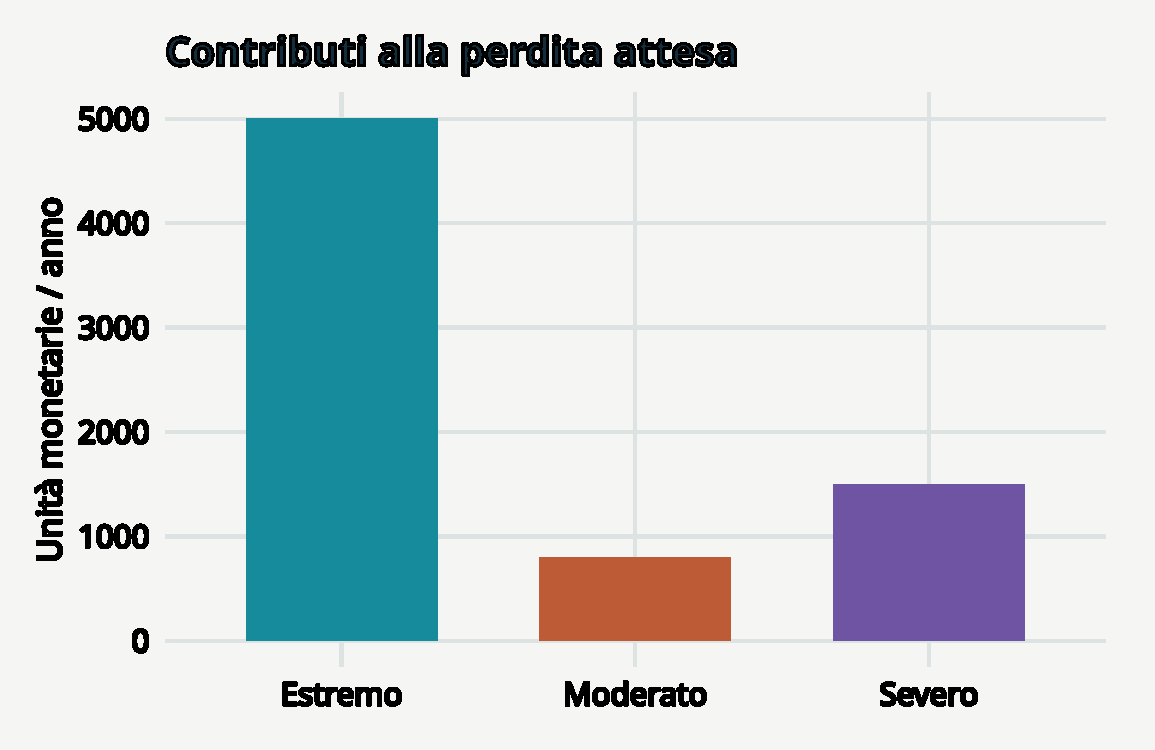
\includegraphics[width=\linewidth,height=6.0cm,keepaspectratio]{Esperimenti/m14-conseguenze-A.pdf}\par}
\PSmall{Moltiplicatore dell’esposizione: 1. Seme: 17.}
}};
\node[anchor=north west,inner sep=0] at([xshift=10.85cm,yshift=-2.12cm]current page.north west){\Colonna{8.16cm}{\PLabel{Scenario A · simulazione}
\PBody{La perdita attesa combina la probabilità di un fenomeno con le conseguenze attribuite al suo verificarsi. L’esperimento distingue tre classi annuali mutuamente esclusive, alle quali assegna probabilità fissate e danni ipotetici; la probabilità restante corrisponde a perdita nulla. I controlli moltiplicano i danni secondo livelli relativi di esposizione e vulnerabilità.}
\par\smallskip{\centering\adjustbox{max width=.98\linewidth}{$\displaystyle E(L)=\sum_kp_kL_k$}\par\smallskip}
\PSmall{$p_k$ è la probabilità annuale della classe k e $L_k$ la perdita associata, dopo l’applicazione dei moltiplicatori. E(L) è la somma dei contributi $p_k L_k$, espressa in unità monetarie per anno.}
}};
\node[anchor=north east,inner sep=0] at([xshift=17.1cm,yshift=-12.04cm]current page.north west){\fontsize{7.7}{9}\selectfont \href{https://marzione00.github.io/Lab_Geo/\#laboratorio/m14-conseguenze}{\color{Classical}\bfseries Apri il laboratorio · m14-conseguenze}};
\end{tikzpicture}\end{frame}

\begin{frame}[plain]\hypertarget{slide64}{}
\bookmark[level=1,page=64]{Confronto | Pericolosità e conseguenze}
\begin{tikzpicture}[remember picture,overlay]
\PilotChrome{Confronto | Pericolosità e conseguenze}{PERICOLOSITÀ, CONSEGUENZE E COMUNICAZIONE}{64}{Il rischio dipende sia dalla frequenza degli eventi sia dalle conseguenze associate.}
\node[anchor=north west,inner sep=0] at([xshift=.96cm,yshift=-2.12cm]current page.north west){\Colonna{9.40cm}{{\centering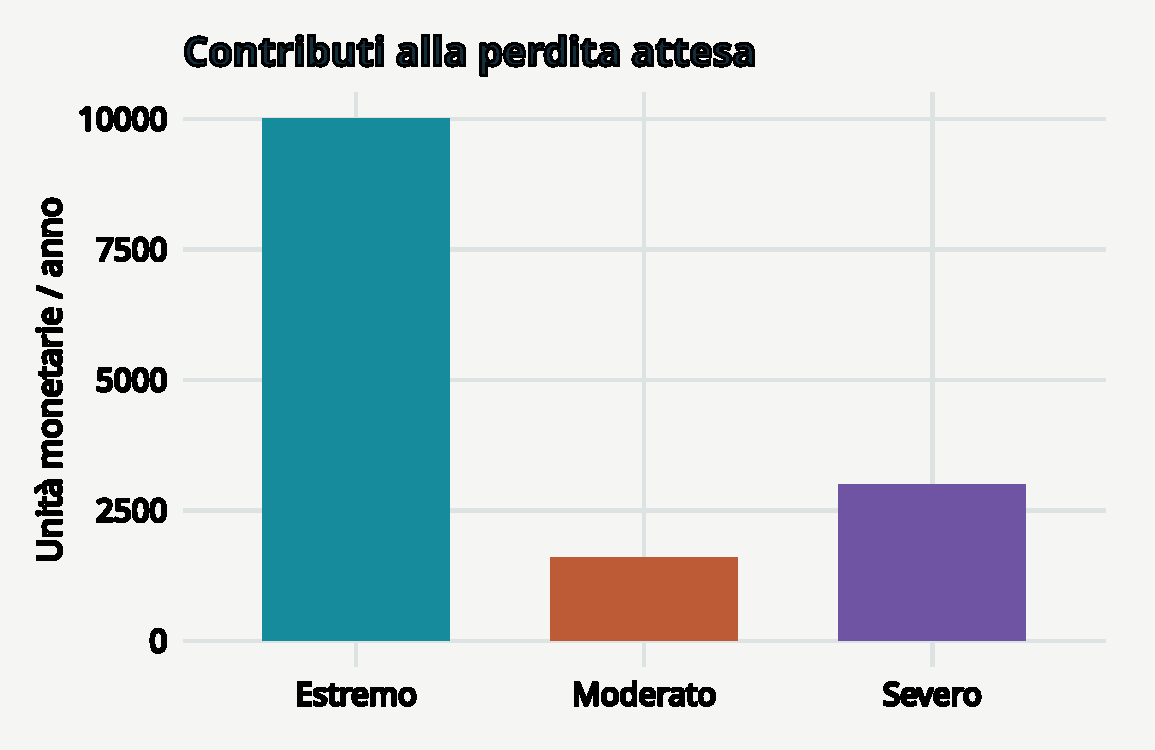
\includegraphics[width=\linewidth,height=5.6cm,keepaspectratio]{Esperimenti/m14-conseguenze-B.pdf}\par}
\PSmall{Moltiplicatore dell’esposizione: 1 $\to$ 2. Tutti gli altri parametri e il seme sono fissi.}
}};
\node[anchor=north west,inner sep=0] at([xshift=10.85cm,yshift=-2.12cm]current page.north west){\Colonna{8.16cm}{\PLabel{Confronto fra gli scenari}
{\fontsize{10.2}{12.8}\selectfont\begin{tabular}{@{}>{\raggedright\arraybackslash}p{0.48\linewidth}@{\hspace{.13cm}}>{\raggedright\arraybackslash}p{0.224\linewidth}@{\hspace{.13cm}}>{\raggedright\arraybackslash}p{0.224\linewidth}@{}}\toprule Grandezza & A & B\\[2.3pt]
\midrule 
Perdita attesa annua & 7300 & 14600\\[2.3pt]
Probabilità annua di una classe dannosa & 0,1 & 0,1\\[2.3pt]
Esposizione relativa & 1 & 2\\[2.3pt]
\bottomrule\end{tabular}\par}
\vspace{.25cm}\PBody{Raddoppiare l’esposizione raddoppia la perdita attesa da 7300 a 14600 unità monetarie. Le probabilità delle classi restano quelle del primo scenario.}
}};
\node[anchor=north east,inner sep=0] at([xshift=17.1cm,yshift=-12.04cm]current page.north west){\fontsize{7.7}{9}\selectfont \href{https://marzione00.github.io/Lab_Geo/\#laboratorio/m14-conseguenze}{\color{Classical}\bfseries Apri il laboratorio · m14-conseguenze}};
\end{tikzpicture}\end{frame}

\begin{frame}[plain]\hypertarget{slide65}{}
\bookmark[level=1,page=65]{Dal risultato alla relazione}
\begin{tikzpicture}[remember picture,overlay]
\PilotChrome{Dal risultato alla relazione}{SINTESI}{65}{Riporta livello, unità, orizzonte, metodo di stima e incertezza insieme.}
\node[anchor=north west,inner sep=0] at([xshift=.96cm,yshift=-2.12cm]current page.north west){\Colonna{9.40cm}{\PLabel{Domanda di partenza}
\PBody{Quale portata associamo a un superamento con probabilità annua dell’uno per cento?}
\PLabel{Risultato da discutere}
\PBody{Il modello Gumbel dei cento massimi sintetici stima il livello centennale a circa 858 m³/s. Sotto indipendenza e stazionarietà la probabilità di almeno un superamento in 50 anni è circa 0,395.}
}};
\node[anchor=north west,inner sep=0] at([xshift=10.85cm,yshift=-2.12cm]current page.north west){\Colonna{8.16cm}{\PLabel{Limiti della conclusione}
\PBody{La stima cambia con la lunghezza del record, il comportamento della coda e le ipotesi fra anni. Un calcolo di danno richiede inoltre esposizione e vulnerabilità.}
\vspace{.4cm}\href{https://marzione00.github.io/Lab_Geo/\#modulo-P09}{\color{Classical}\bfseries Prosegui · P09 · Un livello raro e la sua incertezza}}};
\end{tikzpicture}\end{frame}

\begin{frame}[plain]\hypertarget{slide66}{}
\bookmark[level=1,page=66]{Fonti, dati e codice per riprodurre le figure}
\begin{tikzpicture}[remember picture,overlay]
\PilotChrome{Fonti, dati e codice per riprodurre le figure}{RIFERIMENTI}{66}{I risultati numerici si riferiscono al record e alle ipotesi didattiche dichiarate.}
\node[anchor=north west,inner sep=0] at([xshift=.96cm,yshift=-2.12cm]current page.north west){\Colonna{9.40cm}{\PLabel{Materiali del corso}
\PBody{Il fascicolo deriva dal modulo M14 di GeoStat Lab e dai materiali didattici di Marzio De Corato. I dati del caso guida sono didattici. Le simulazioni A e B riportano il proprio seme.}
\href{https://github.com/marzione00/Lab_Geo/blob/649f7cc577b96bd1044d81e78a2f530813e4f96b/moduli/M14/README.md}{\color{Classical}\bfseries Scheda e documentazione originale}\par\smallskip \href{https://github.com/marzione00/Lab_Geo/blob/649f7cc577b96bd1044d81e78a2f530813e4f96b/materiali/R/M14_figure.R}{\color{Classical}\bfseries Script R delle figure del corso}}};
\node[anchor=north west,inner sep=0] at([xshift=10.85cm,yshift=-2.12cm]current page.north west){\Colonna{8.16cm}{\PLabel{Nell’archivio dei sorgenti}
\PBody{Codice contiene i frammenti delle pagine. Esperimenti comprende i due programmi R e i risultati di ciascun confronto. Diagrammi contiene i disegni TikZ modificabili. Scena conserva il modello Blender della copertina.}
\vspace{.4cm}\href{https://marzione00.github.io/Lab_Geo/\#modulo-M14}{\color{Classical}\bfseries Apri Ignis su GeoStat Lab}}};
\end{tikzpicture}\end{frame}

\end{document}